\ifnum\aluno=1
\renewcommand\chapterillustration{./abertura-exponencial}
\else
\renewcommand\chapterillustration{./abertura-exponencial-professor}
\fi
\renewcommand\chapterwhat{Crescimento e decaimento exponenciais, função exponencial, juros compostos, progressão geométrica, expoentes racionais e irracionais.}
\renewcommand\chapterbecause{Dizemos que estamos diante de um crescimento exponencial sempre que o aumento percentual de determinada quantidade por unidade de tempo é constante. Este é o caso das medições econômicas, financeiras e políticas de crescimento - de vendas, lucros, preços de ações, produto interno bruto, inflação, taxas de juros. Assim, compreender bem o crescimento exponencial é crucial para compreender o mundo.}
\chapter{Função Exponencial}



\mbox{}\thispagestyle{empty}\clearpage

\thispagestyle{empty}

\begin{center}
Projeto: LIVRO ABERTO DE MATEMÁTICA

 \begin{tabular}{lcccr}

\includegraphics[scale=.15]{impa}& \quad\quad& 
\includegraphics[width=3cm]{logo} & \quad\quad& 
\includegraphics[scale=.24]{obmep} 
\end{tabular}
\end{center}

\vspace*{.3cm}

Cadastre-se como colaborador no site do projeto: \url{umlivroaberto.com}

Versão digital do capítulo:

\url{https://www.umlivroaberto.org/BookCloud/Volume_1/master/view/AF107.html}


\begin{tabular}{p{.15\textwidth}p{.7\textwidth}}
Título: & Função Exponencial\\
\\
Ano/ Versão: & 2019 / versão 0.1 de 23 de outubro de 2020\\
\\
Editora & Instituto Nacional de Matem\'atica Pura e Aplicada (IMPA-OS)\\
\\
Realização:& Olimp\'iada Brasileira de Matem\'atica das Escolas P\'ublicas (OBMEP)\\
\\
Produção:& Livro Aberto\\
\\
Coordenação:& Fabio Simas e Augusto Teixeira (livroaberto@impa.br)\\
\\
  Autores: & Gladson Antunes (UNIRIO),\\
        & Michel Cambrainha (UNIRIO)\\
\\
Revisoras: &  Cydara Ripoll  \\
                &  Letícia Rangel \\
\\
Design: & Andreza Moreira (Tangentes Design) \\
\\
  Ilustrações: & --- \\ 
\\
Gráficos: & Beatriz Cabral e Tarso Caldas (Licenciandos da UNIRIO)\\
\\
  Capa: & Foto de Gustavo Fring , no Pexels \\

\end{tabular}


\begin{figure}[b]
\begin{minipage}[l]{5cm}
\centering

{\large Licença:}

  
\includegraphics[width=3.5cm]{cc-by-nc-sa}
\end{minipage}\hfill
\begin{minipage}[c]{5cm}
\centering
{\large Desenvolvido por}


\includegraphics[width=2.5cm]{logo-associacao.jpg}
\end{minipage}
\begin{minipage}[r]{5cm}
\centering

{\large Patrocínio:}
  \vspace{1em}
  
\includegraphics[width=3.5cm]{itau}
\end{minipage}
\end{figure}

\mainmatter

\begin{apresentacao}
\section{Função Exponencial}

As ideias que envolvem as funções exponenciais (e logarítmicas) estão entre as mais comuns na ciência e ao mesmo tempo são as que oferecem os maiores desafios aos professores e estudantes, especialmente na Educação Básica. São ideias impregnadas de sutilezas conceituais e epistemológicas e que, para quase a totalidade dos docentes, passam despercebidas, fazendo com que o ensino desse tópico acabe por ficar reduzido a memorizações e procedimentos mecânicos. Como se trata de um assunto desafiador para ambos estudantes e professores, torna-se mais difícil antecipar as dificuldades dos estudantes e como consequência não há espaço para refletir sobre que ações tomar para superar tais dificuldades. \citep{Davis2009}; \citep{Weber2002}

Durante os anos do Ensino Fundamental o estudante aprende a lidar com a potenciação considerando-a como uma nova operação/notação para indicar a multiplicação repetida (potências que envolvem expoentes naturais). No Ensino Médio, entretanto, ele deve ser capaz de extrapolar esse conceito e generalizá-lo de duas maneiras não triviais: (1) fazer a transição da multiplicação repetida $(2^{3}=2 \times 2 \times 2 )$ para a correspondência ou função cujo domínio é o conjunto dos números naturais $(n \longrightarrow 2^{n})$ estender para expoentes inteiros, racionais e irracionais, de maneira a dar significado para essas extensões. Infelizmente, como documentam diversas pesquisas relacionadas a este tema, esse objetivo raramente é atingido com sucesso.  Davis (2009) aponta que a perspectiva de multiplicação repetida impõe dificuldades aos estudantes quando se deparam com expoentes não inteiros.

É fundamental que os alunos sejam capazes de entender a exponenciação como um processo matemático e as expressões exponenciais como objetos matemáticos que são o resultado desse processo. \citep{Weber2002}

O conceito de função exponencial está intimamente relacionado com os juros compostos e as progressões geométricas e raramente essas conexões (especialmente com as P.G.) são bem exploradas nos livros didáticos brasileiro. Pretendemos neste livro fazer as conexões entre tais tópicos que são explicitamente apontada pela BNCC \citep{BNCC2018} (EM13MAT304, EM13MAT508). 

Tradicionalmente a função exponencial é apresentada nos livros didáticos na sua forma, digamos, mais sucinta: $f(x)=a^x$. Neste capítulo, optamos por apresentar a função exponencial na forma $f(x) = c \cdot a^x$, porque entendemos que esse formato se mostra mais conveniente nos modelos matemáticos de situações reais. A constante $c$ comumente é explicitada (ou solicitada) nos problemas como a quantidade/valor inicial. Também fica mais simples fazer a relação com os problemas de Progressões Geométricas cuja fórmula do termo geral contém o primeiro termo multiplicando a potência ($a_{n+1}=a_1\cdot q^n$). 
Matematicamente, tanto é possível considerar o caso $f(x)=a^x$ como um caso particular do outro, em que a constante $c=1$, quanto considerar que o caso $f(x)=c\cdot a^x$ é obtido do outro realizando-se uma translação na variável do domínio:
\[
f(x)=c\cdot a^x = a^{\log_a c} \cdot a^x = a^{x + \log_a c}=a^{x+k}
\]
Uma outra observação importante é que por conta das aplicações, consideramos para a função exponencial apenas os casos em que $c>0$. Isso também evita algumas confusões em relação ao crescimento e decrescimento das funções: note que para $c<0$, a função $f(x)=c\cdot a^x$ é crescente se, somente se, $0<a<1$.

\section*{Objetivos Gerais}

\begin{itemize}
\item {} Diferenciar situações de crescimento e decaimento exponenciais;

\item {} Reconhecer situações que podem ser modeladas por uma função exponencial $f(x)=c \cdot a^{x}$, identificando $c$ como o valor inicial e $a$ como fator de crescimento, e propor modelos;

\item {} Transitar entre as diferentes representações para a função exponencial: tabelas, fórmulas, gráficos, problemas textuais;

\item {} Associar as progressões geométricas a funções exponenciais de domínios discretos;

\item {} Apresentar o número $e$.
\end{itemize}

\section*{Habilidades da BNCC}

\begin{habilities}{EM13MAT304} 
Resolver e elaborar problemas com funções exponenciais nos quais seja necessário compreender e interpretar a variação das grandezas envolvidas, em contextos como o da Matemática Financeira, entre outros.

\tcbsubtitle{EM13MAT403}
Analisar e estabelecer relações, com ou sem apoio de tecnologias digitais, entre as representações de funções exponencial e logarítmica expressas em tabelas e em plano cartesiano, para identificar as características fundamentais (domínio, imagem, crescimento) de cada função.

\tcbsubtitle{EM13MAT508}
Identificar e associar progressões geométricas (PG) a funções exponenciais de domínios discretos, para análise de propriedades, dedução de algumas fórmulas e resolução de problemas.
\end{habilities}

\section*{Pré-requisitos}

\begin{habilities}{EF08MA01} 
Efetuar cálculos com potências de expoentes inteiros e aplicar esse conhecimento na representação de números em notação científica. Potenciação e radiciação.

\tcbsubtitle{EF08MA02} 
Resolver e elaborar problemas usando a relação entre potenciação e radiciação, para representar uma raiz como potência de expoente fracionário.

\tcbsubtitle{EF09MA02} 
Reconhecer um número irracional como um número real cuja representação decimal é infinita e não periódica, e estimar a localização de alguns deles na reta numérica.

\tcbsubtitle{EF09MA03} 
Efetuar cálculos com números reais, inclusive potências com expoentes fracionários.
\end{habilities}

\section*{Distratores}

\begin{itemize}

\item Estudantes de nível superior têm dificuldades em entender e explicar as regras da exponenciação e não são capazes de conectá-las às regras do logaritmo. Não conseguem explicar o que significa uma função do tipo $f(x)=ax$, nem justificar porque uma função do tipo $f(x)=\left(\dfrac{1}{2} \right)^{x}$ é decrescente. \citep{Weber2002}

\item Em geral os professores são capazes de fazer uso das representações gráfica, algébrica e tabular, no entanto isso não implica necessariamente conhecimento conceitual acerca das funções exponenciais. \citep{Presmeg2005}

\item Estudantes do ensino fundamental apresentam dificuldades em fazer a transição das representações lineares para as exponenciais, ou em identificar o que torna os dados exponenciais. \citep{Alagic2006}

\item Abordagens tradicionais do ensino de funções apoiam-se em uma visão de correspondência, na qual uma função é vista como uma relação estática entre os elementos de dois conjuntos. Essa visão estática está na base da maneira como esse tema é tratado na matemática escolar, e não é difícil perceber como os estudantes lutam para fazer a transição do entendimento da multiplicação repetida para a ideia de correspondência em um domínio de números naturais. \citep{Ellis2012}

\item Na matemática escolar, qualquer propriedade que é válida para números irracionais é automaticamente considerada válida para números irracionais, sem justificativas matemáticas. \citep{Wu2011}

\end{itemize}

O capítulo está organizado da seguinte forma: a primeira seção aborda situações-problema em que se observa crescimento ou decaimento exponencial. O objetivo dessa seção é que os estudantes aprendam o vocabulário básico e reconheçam os padrões exponenciais em textos, tabelas, gráficos e equações, com destaque para o papel do fator de crescimento e do valor inicial nas expressões exponenciais. É esperado também nessa seção que os estudantes consigam deduzir fórmulas que modelem esse tipo de crescimento/decaimento e representem graficamente os dados de um problema ou situação real.

A seção 2 tem como objetivo apresentar uma outra maneira de expressar a variação exponencial: por meio de taxas percentuais. Novos problemas são apresentados, mas agora com essa linguagem que expressa o fator de crescimento como aumento ou diminuição percentual em relação aos valores anteriores. A relação entre a taxa ($r$) e o fator de multiplicação ($1+r$) é explorada em algumas situações incluindo as que envolvem juros e transações financeiras.

Na seção 3 apresentamos, de fato, a função exponencial. Começamos com atividades que recordam as propriedades dos expoentes naturais, inteiros e racionais para, em seguida, fazer a passagem para os expoentes irracionais. Representações gráficas e as relações das propriedades com os parâmetros em expressões completas do tipo $f(x)=c\cdot a^{\frac xd}$ são também exploradas nesta seção.

A próxima seção é dedicada a explorar a taxa de variação da função exponencial, evidenciando que ela supera todos os outros crescimentos que já foram estudados. A seção termina com a construção do número de Euler em situações de crescimento contínuo.

A última seção é dedicada ao estudo das Progressões Geométricas e como elas se relacionam com as funções exponenciais. De fato, todas as ideias principais são desenvolvidas ao longo de todo o capítulo (em situações onde se observa crescimento/decaimento exponencial em domínios discretos), mas apenas neste as traduzimos para a linguagem de sequências. O conceito de PG é um pouco mais amplo, por incluir sequências em que o primeiro termo ou a razão são negativos. Essa ressalva é feita em algumas atividades. As últimas atividades tratam das somas de termos de uma PG estabelecendo uma relação dessas somas com problemas geométricos.
\end{apresentacao}

\clearpage
\def\currentcolor{session1}
\begin{texto}
{	
	\section{Explorando: Crescimento e Decaimento Exponenciais}
	Nesta seção iremos explorar as ideias de crescimento e decaimento exponenciais, apresentando alguns contextos onde esse tipo de variação aparece naturalmente.

	Por enquanto, vamos nos restringir a expoentes inteiros positivos, aproveitando a oportunidade para revisar algumas propriedades operatórias das potências. Outros expoentes serão tratados mais adiante, na seção (retornar e informar a seção).

	O material foi concebido de forma a contribuir para a ampliação da visão do estudante sobre a exponenciação, fazendo com que ele deixe de vê-la apenas como multiplicação repetida (ação), passando a enxergá-la como resultado de uma transformação ou de uma correspondência entre conjuntos (processo), podendo operar com as exponenciais sem necessariamente “efetuar a operação”. Esse entendimento conduz o estudante a conclusões como $3^{x}$ é sempre um número positivo para $x$ inteiro positivo, pois você começa com $3$ e segue sempre multiplicando por um número positivo, ou que a correspondência gera uma sequência (função) crescente, ou ainda a compreender as propriedades tais como $5^{x} \cdot 5^{y} = 5^{x+y}$, dentre outras. (WEBER, 2002)

	Neste primeiro momento sugerimos não antecipar as propriedades que envolvem os expoentes negativos e racionais para que isso não afete a construção das ideias mais adiante.

	Ao introduzir este assunto, caso haja disponibilidade, sugerimos compartilhar com a turma o vídeo \url{https://youtu.be/s-lgS-4Xqy0}, em que a ideia de crescimento exponencial é exemplificada por meio do crescimento de Vitórias-Régias.
}
\end{texto}
\begin{objectives}{A epidemia}
{
	\begin{itemize}
	\item Simular uma situação de crescimento exponencial;
	\item Reconhecer padrões exponenciais em tabelas, gráficos, identificando o papel do fator de crescimento.
	\end{itemize}
}{1}{1}
\end{objectives}
\clearmargin
\begin{sugestions}{A epidemia}
{
	\begin{itemize}
	\item Caso deseje peça anteriormente que seus estudantes realizem uma pesquisa sobre epidemias, pandemias, endemias. Pode ser um trabalho realizado em conjunto com outras disciplinas como Geografia, Sociologia, Biologia.
	\item Esta atividade trata de um dos Temas Contemporâneos Transversais da BNCC: Saúde. E com potencial para tratar de “Vida Familiar e Social” e “Trabalho”.
	\item Para uma melhor visualização, considere organizar os estudantes em círculo
	\item É muito importante anotar os números na lousa e ir apagando à medida em que forem sendo escolhidos, para ajudar os novos infectados a escolher suas vítimas.
	\item Escolha um estudante para ser o pesquisador e anotar os dados no quadro.
	\item Ao final de cada rodada pergunte à turma como evoluiria o total de infectados nas próximas rodadas caso houvesse mais alunos na turma.
	\item Para responder o item (e) você pode consultar a população da sua cidade e estado neste link (\url{https://www.ibge.gov.br/estatisticas/sociais/populacao/9103-estimativas-de-populacao.html?=&t=resultados})
	\item Adaptado de BUSH, S., GIBBONS, K., KARP, K., DILLON, F. Epidemics, exponential function and modelling, Mathematics Teaching in the Middle School, Vol. 21, No. 2, pp. 90-97, 2015.
	\end{itemize}
}{1}{2}
\end{sugestions}
\begin{answer}{A epidemia}
{
	\begin{enumerate}
\item {} 
Tabela com o número de infectados até a rodada 8.

\begin{tabular}{|c|c|c|c|}
\hline
\tcolor{Rodada} & \tcolor{Epidemia 1} & \tcolor{Epidemia 2} & \tcolor{Epidemia 3} \\ \hline
0      & 2          & 3          & 1          \\ \hline
1      & 4          & 6          & 3          \\ \hline
2      & 8          & 12         & 9          \\ \hline
3      & 16         & 24         & 27         \\ \hline
4      & 32         & 48         & 81         \\ \hline
5      & 64         & 96         & 243        \\ \hline
6      & 128        & 192        & 729        \\ \hline
7      & 256        & 384        & 2187       \\ \hline
8      & 512        & 768        & 6561       \\ \hline
\end{tabular}

\item\adjustbox{valign=t}
{
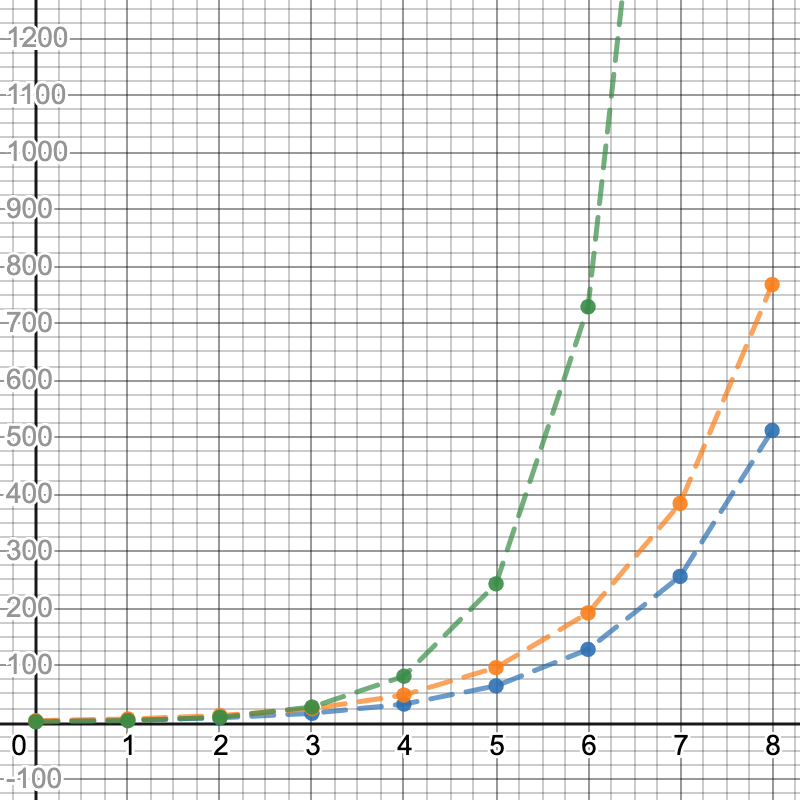
\includegraphics[width=.7\linewidth]{epidemias.png}
}

\item{}
Uma resposta possível é dizer que nas epidemias $1$ e $2$ a cada rodada o número de infectados dobra. Na epidemia $3$ o número de infectados triplica a cada rodada.

\item{}
A informação solicitada depende do número de estudantes da escola.

\item{}
As informações solicitadas dependem de informações sobre a população da cidade, estado e país.

\end{enumerate}
}{0}
\end{answer}
\clearmargin
\begin{objectives}{Contando quadrados}
{
	\begin{itemize}
\item Investigar um modelo discreto de decaimento exponencial;
\item Identificar gráficos de funções exponenciais decrescentes e relacionar ao fator de crescimento;
\item Reconhecer o modelo exponencial em dados experimentais.
\end{itemize}
}{1}{1}
\end{objectives}
\begin{sugestions}{Contando quadrados}
{
	\begin{itemize}
	\item Esta atividade é uma adaptação do experimento \textit{Eliminando Quadrados} (\url {https://m3.ime.unicamp.br/recursos/1008}) que faz parte da coleção  Matemática Multimídia da UNICAMP (\url{https://m3.ime.unicamp.br}) que oferece diversos recursos educacionais de Matemática para o ensino médio.
	\item No item \titem{d)} as perguntam visam estimular conjecturas do tipo os números são sempre positivos, sempre menores que um, eventualmente são iguais a 0 ou 1, mas isso ocorre apenas para quantidades pequenas de quadradinhos, ficam próximos de $0{,}5$, etc. Estimule que eles registrem as razões que os levaram a tais conjecturas.
	\item Discuta sobre o que ocorreria caso o número de quadradinhos fosse bem maior; veja se há interesse na turma em desenvolver um projeto de programação que simule os lançamentos.
	\end{itemize}
}{1}{1}
\end{sugestions}
\begin{answer}{Contando quadrados}
{
	\begin{enumerate}
	\item {} 
	\adjustbox{valign=t}
	{
	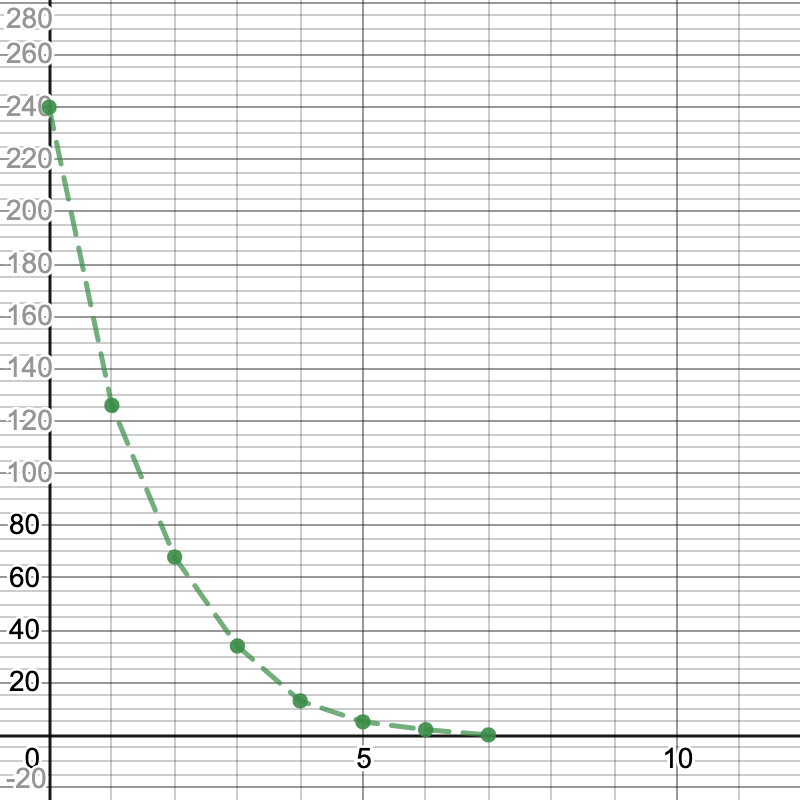
\includegraphics[width=.6\linewidth]{Contando_quadrados.png}
	}

	\end{enumerate}
}{1}
\end{answer}
\clearmargin
\begin{answer}{Contando quadrados}
{
	\begin{enumerate}\setcounter{enumi}{1}
	\item{}
	Observa-se que o número de quadrados com a face verde voltada para cima fica entre $40$ e $50\%$ do valor anterior a cada lançamento. O valor zero do final acontece por causa da quantidade pequena de quadrados.

	\item{}
	\adjustbox{valign=t}
	{
	\begin{tabu} to \textwidth{|c|c|c|}
	\hline
	\tcolor{Lançamento} & \tcolor{\# verdes} & \tcolor{quocientes} \\ 
	\hline
	0 & $240$ & --- \\ 
	\hline
	1 & $126$ & $\frac{126}{240}=0{,}525$\\ 
	\hline
	2 & $68$ & $\frac{68}{126}\approx0{,}539$ \\ 
	\hline
	3 & $34$ & $\frac{34}{68}=0{,}5$ \\ 
	\hline
	4 & $13$ & $\frac{13}{34}\approx 0{,}382$\\ 	
	\hline
	5 & $5$ & $\frac{5}{13}\approx 0{,}384$\\ 
	\hline
	6 & $2$ & $\frac{2}{5}=0{,}4$\\ 
	\hline
	7 & $0$ & $\frac{0}{2}=0$\\ 
	\hline
	\end{tabu}
	}

	\item{}
	Algumas respostas possíveis: serão sempre números positivos, sempre menores ou iguais a um, o quociente tende a ficar próximo a $0,5$.

	\item{}
	Responder em concordância com o que foi conjecturado no item anterior.

	\item{}
	Expressão da forma $F(n)=240\times a^{n}$, em que $a$ é qualquer valor próximo a $0,5$.

	\end{enumerate}
}{1}
\end{answer}
\begin{objectives}{Populações}
{
	\begin{itemize}
	\item Deduzir uma equação exponencial a partir da identificação do valor inicial e do fator de crescimento/decaimento;

	\end{itemize}
}{1}{2}
\end{objectives}
\begin{sugestions}{Populações}
{
	\begin{itemize}
	\item O site do Instituto Chico Mendes de Conservação da Biodiversidade (ICMBio) apresenta uma classificação de acordo com o grau do risco de extinção de uma espécie. Ela pode ser acessada neste endereço: \url{https://www.icmbio.gov.br/ran/images/Arquivos/especies_ameacadas/categorias_criterios_iucn_2012.pdf}.\\ Pode ser um tema interessante a ser discutido também com o professor de Biologia.
	\end{itemize}
}{1}{2}
\end{sugestions}
\begin{answer}{Populações}
{
	\begin{enumerate}

	\item{}
	$P(n)=300000 \times \left(\dfrac{1}{3}\right)^{n}$.

	\item{}
	Ao final do quinto ano.

	\item{}
	$p(n)=5 \times10^{5} \times 4^{n}$.

	\end{enumerate}
}{0}
\end{answer}

\explore{Crescimento e decaimento exponenciais}%\label{credecai}

A pandemia de COVID-19, uma doença respiratória aguda provocada pelo coronavírus SARS-CoV-2, chamou atenção do mundo todo em 2020 para o que chamamos de crescimento exponencial. Vimos diversos especialistas em diferentes meios de comunicação comentando sobre o crescimento exponencial da epidemia. Mas afinal, o que caracteriza este tipo de crescimento?

\begin{figure}[H]
\centering

\includegraphics[width=.75\textwidth]{reportagem.png}
%\caption{}
\end{figure}


Sabemos que funções matemáticas podem ser usadas para fazermos previsões de um determinado fenômeno. A função exponencial fornece um modelo matemático simples para calcular a propagação de uma doença altamente contagiosa. Para além disso, o gráfico de uma função exponencial permite o estudo de situações que se caracterizam por uma curva de crescimento ou decrescimento acentuado. Neste capítulo você irá aprender a identificar, elaborar e resolver problemas que envolvem funções exponenciais. Além da modelagem de epidemias, serão apresentadas situações que envolvem decaimento radioativo, meia-vida de medicamentos, pressão atmosférica, divisão celular, dentre outras aplicações interessantes.

\begin{task}{A epidemia}


Vamos simular três situações de epidemia. O professor irá distribuir envelopes contendo um número para cada estudante que deverá mantê-lo em segredo. Os primeiros infectados serão escolhidos ao acaso pelo professor. Cada vez que alguém for infectado pela doença, coloca-se de pé e permanece até o fim da dinâmica, que seguirá da seguinte maneira:

\begin{figure}[H]
\centering

\includegraphics[width=300bp]{epidemia.png}
%\caption{https://youtu.be/s-lgS-4Xqy0}
\end{figure}


\subsection{Epidemia 1}

\begin{itemize}

\item RODADA 0: O professor escolhe dois números para serem os primeiros infectados, diz seus números e apaga-os da lista que está escrita na lousa. Os infectados ficam de pé. O pesquisador anota o número de infectados.

\item RODADA 1: Cada um dos infectados escolhe um número que não tenha sido sorteado para “infectar”; os números são apagados na lousa e somente depois de todos terem escolhido suas vítimas, os novos infectados se colocam de pé. O pesquisador anota o número total de infectados.

\item RODADA 2: Semelhante à rodada 1.

\item As rodadas seguem até que todos tenham sido infectados.

\end{itemize}

% 

\subsection{Epidemia 2}

\begin{itemize}

\item A mesma dinâmica anterior, porém começando com três infectados na rodada 0.

\end{itemize}

\subsection{Epidemia 3}
\begin{itemize}

\item Apenas um infectado na rodada 0 e cada infectado agora escolhe dois números para infectar a cada rodada.

\end{itemize}

Responda às seguintes perguntas:

\begin{enumerate}
\item{} 
Anote os dados das três epidemias em tabelas e faça previsões para 4 rodadas além das que efetivamente ocorreram na sua turma.

\item{} 
Represente os dados graficamente.

\item{} 
Que critérios você usou no item (a) para fazer suas previsões? Qual a relação deles com os dados específicos de cada uma das epidemias.

\item{}
Quantas rodadas aproximadamente demoraria para cada epidemia infectar todos os estudantes da sua escola? Primeiro faça um “chute” e somente depois faça as contas.

\item{}
Responda a mesma pergunta anterior considerando a sua cidade, seu estado e o todo o país.

\end{enumerate}
\end{task}

\clearpage
\begin{task}{Contando quadrados}

Em uma caixa há $240$ quadradinhos de papel cartão dupla face, verde de um lado e marrom do outro. Eles são lançados sobre a mesa e os quadrados com lado marrom para cima são retirados, restando apenas $126$ quadradinhos (verdes).

\begin{figure}[H]
\centering
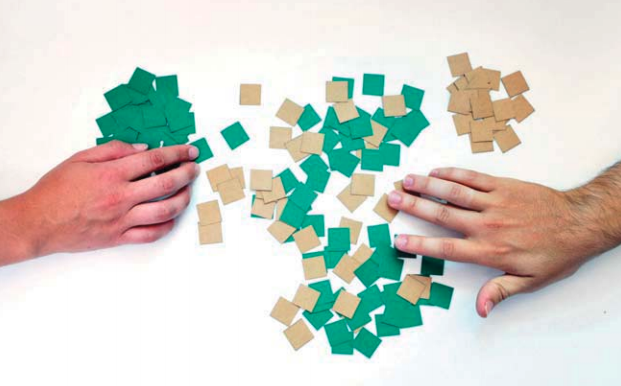
\includegraphics[width=250bp]{eliminando_quadrados.png}
\caption{Imagem retirada do experimento \textit{Eliminando Quadrados}, da coleção Recursos educacionais multimídia para a matemática do ensino médio. \url{https://m3.ime.unicamp.br/recursos/1008} }
\end{figure}


Um novo lançamento é feito e depois de retirados os marrons, sobram 68 verdes. Os lançamentos seguintes apresentam as seguintes quantidades de quadradinhos verdes:

\begin{center}
\begin{tabular}{|c|c|}
\hline
\tcolor{Lançamento} & \tcolor{\# verdes} \\ \hline
0 & $240$ \\ 
\hline
1 & $126$ \\ 
\hline
2 & $68$ \\ 
\hline
3 & $34$ \\ 
\hline
4 & $13$ \\ 
\hline
5 & $5$ \\ 
\hline
6 & $2$ \\ 
\hline
7 & $0$ \\ 
\hline
\end{tabular}
\end{center}

\begin{enumerate}

\item {}
Represente em um sistema de coordenadas os dados da tabela acima.

\item {}
Observando os dados da tabela é possível conjecturar que eles obedecem a algum padrão?

\item {} 
Acrescente uma terceira coluna à tabela contendo os quocientes entre as quantidades de um lançamento pela quantidade do lançamento anterior.

\begin{center}
\begin{tabular}{|c|c|c|}
\hline
\tcolor{Lançamento} & \tcolor{\# verdes} & \tcolor{quocientes} \\ 
\hline
0 & $240$ & --- \\ 
\hline
1 & $126$ & $\frac{126}{240}=0{,}525$\\ 
\hline
2 & $68$ & \\ 
\hline
3 & $34$ & \\ 
\hline
4 & $13$ &\\ 
\hline
5 & $5$ & \\ 
\hline
6 & $2$ & \\ 
\hline
7 & $0$ & \\ 
\hline
\end{tabular}
\end{center}

\item {}
Considerando outros resultados possíveis para o mesmo experimento, o que podemos esperar dos valores na terceira coluna da tabela? Que tipo de propriedades matemáticas esses números sempre terão? Que tipo de propriedade eles provavelmente terão?

\item {}
Um experimento como este descrito no item (a) pode ser simulado computacionalmente. Ao executar esta simulação 4 vezes, os seguintes resultados foram obtidos. 

$240, 113, 55, 28, 13, 7, 3, 0$ 

$240, 124, 66, 27, 16, 7, 3, 2, 2, 2, 0$ 

$240, 106, 57, 19, 9, 5, 1, 0$ 

$240, 124, 62, 29, 11, 5, 2, 1, 1, 0$

\item {}
Verifique se suas conjecturas se aplicam aos dados acima.

\item {}
Deduza uma expressão matemática que forneça, aproximadamente, a quantidade de quadradinhos verdes em função da ordem de lançamento.

\end{enumerate}

\end{task}

\begin{task}{Populações}

Um grupo de biólogos está estudando uma espécie animal cuja população vem diminuindo ao longo dos anos. Depois de reunirem os dados percebem que a cada ano a quantidade de indivíduos reduz para aproximadamente $\dfrac{1}{3}$ da quantidade do ano anterior.

\begin{enumerate}

\item {}
Escreva uma expressão matemática que relaciona o número de indivíduos dessa população ao longo dos anos, sabendo que no início das medições os cientistas tenham encontrado $300$ mil indivíduos.

\item {}
Admitindo que esse padrão se repita ao longo dos anos, em quanto tempo a população entrará em extinção?

\item {}
Como consequência, a população da espécie que é a principal presa da espécie estudada apresentou um crescimento que duplicava a cada 6 meses. Escreva uma expressão matemática que represente a variação anual do número de indivíduos dessa população de presas, que no início das medições contava com $5\times10^5$ indivíduos.

\end{enumerate}

\end{task}

\arrange{Crescimento e decaimento exponenciais}
%Nos capítulos anteriores conhecemos diversas situações e fenômenos descritos por funções lineares ou polinomiais. No entanto, há muitas outras situações em que estas funções não se mostram as mais adequadas para a modelagem. Mas que situações seriam estas? Pelo que foi visto nas atividades anteriores, são aquelas para as quais observamos um \textbf{rápido crescimento} ou um \textbf{rápido decrescimento}. Situações e fenômenos com estas características são abundantes nas mais diferentes áreas do conhecimento, conforme vimos no início deste capítulo as curvas que representam o crescimento do número de infectados em epidemias é uma curva exponencial.

Há diversas situações bastante comuns na natureza que não são bem modeladas pelas funções que estudamos até agora: as lineares, afins e quadráticas. As três atividades vistas do início deste capítulo exemplificam algumas delas. Uma característica que todas têm em comum é que os valores da variável dependente crescem ou decrescem muito rápido. Essa característica em uma situação real pode indicar que provavelmente estamos diante de uma situação de crescimento (ou decaimento) exponencial. Veja o gráfico abaixo com o número de casos acumulados de COVID-19 no Brasil de março até agosto de 2020. Perceba o tempo aproximado que levamos para alcançar $200.000$ casos ($ \approx $ 3 meses) e o tempo para os novos $200.000$ casos (menos de 15 dias).

\begin{figure}[H]
\centering
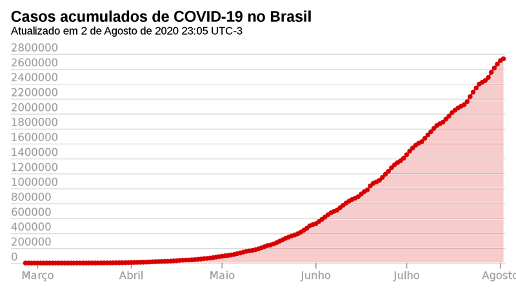
\includegraphics[width=300bp]{covid_brasil.png}
\caption{Fonte: \href{https://pt.wikipedia.org/wiki/Ficheiro:Casos_acumulados_de_COVID-19_no_Brasil.svg}{Wikipedia}}

\end{figure}

Como, afinal identificamos o crescimento (ou decaimento) exponencial? Em todos os casos analisados nas atividades da seção anterior, observamos dois ingredientes fundamentais: um \textbf{valor inicial} para a variável dependente, decorrente da primeira medição, e um \textit{valor constante positivo} que servia como \textbf{fator de multiplicação} para se obter os valores seguintes.

\begin{figure}[H]
\centering
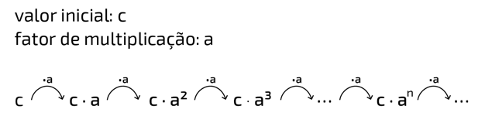
\includegraphics[width=300bp]{esquema.png}
\caption{Crescimento/decrescimento exponenciais.}
\end{figure}

A expressão $f(x)=c\cdot a^{x}$,em que $a$ e $c>0$ são constantes e  é a que usamos para modelar as situações em que há crescimento/decaimento exponencial.

Quando este fenômeno ocorre estamos diante do \textbf{crescimento exponencial}, caso o fator de multiplicação seja maior que 1
\[
a > 1 \Longleftrightarrow a^{2} > a \Longleftrightarrow  a^{3} > a^{2} \Longleftrightarrow \cdots,
\]
ou \textbf{decaimento exponencial} quando o fator está entre 0 e 1.
\[
0< a < 1 \Longleftrightarrow a^{2} < a \Longleftrightarrow  a^{3} < a^{2} \Longleftrightarrow \cdots
\]

\begin{figure}[H]
\centering
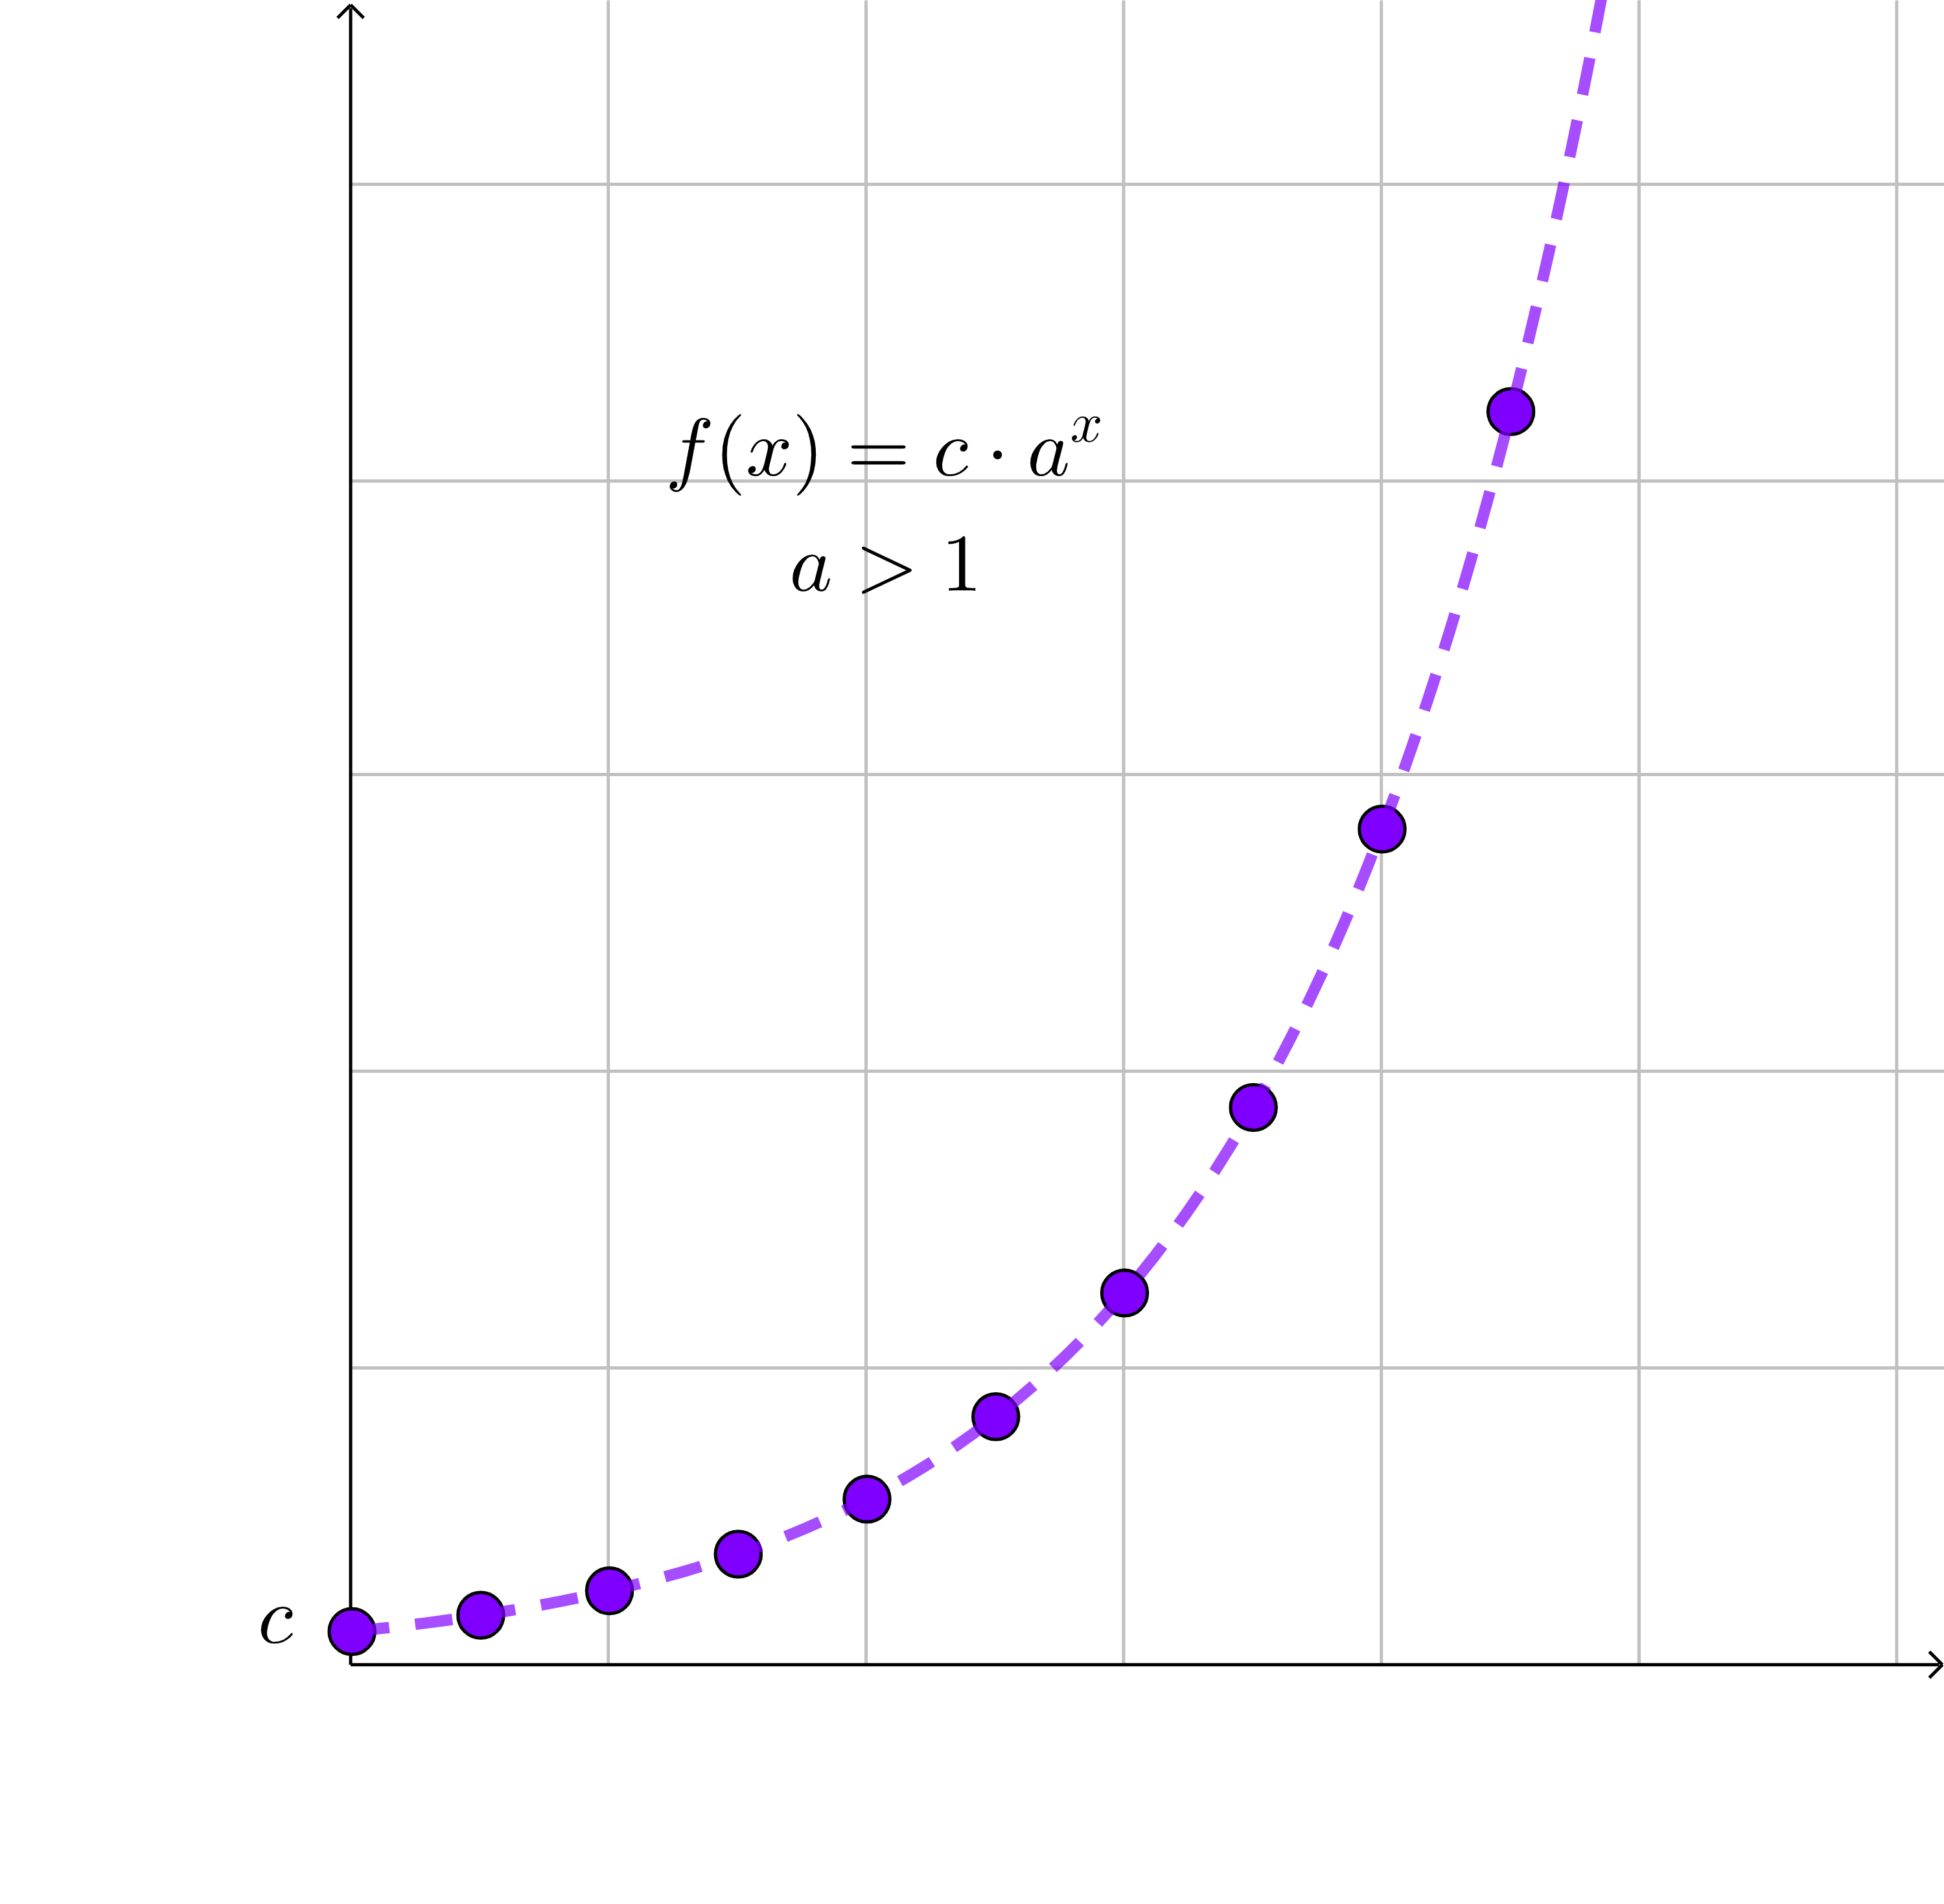
\includegraphics[width=200bp]{exp_cresc.png}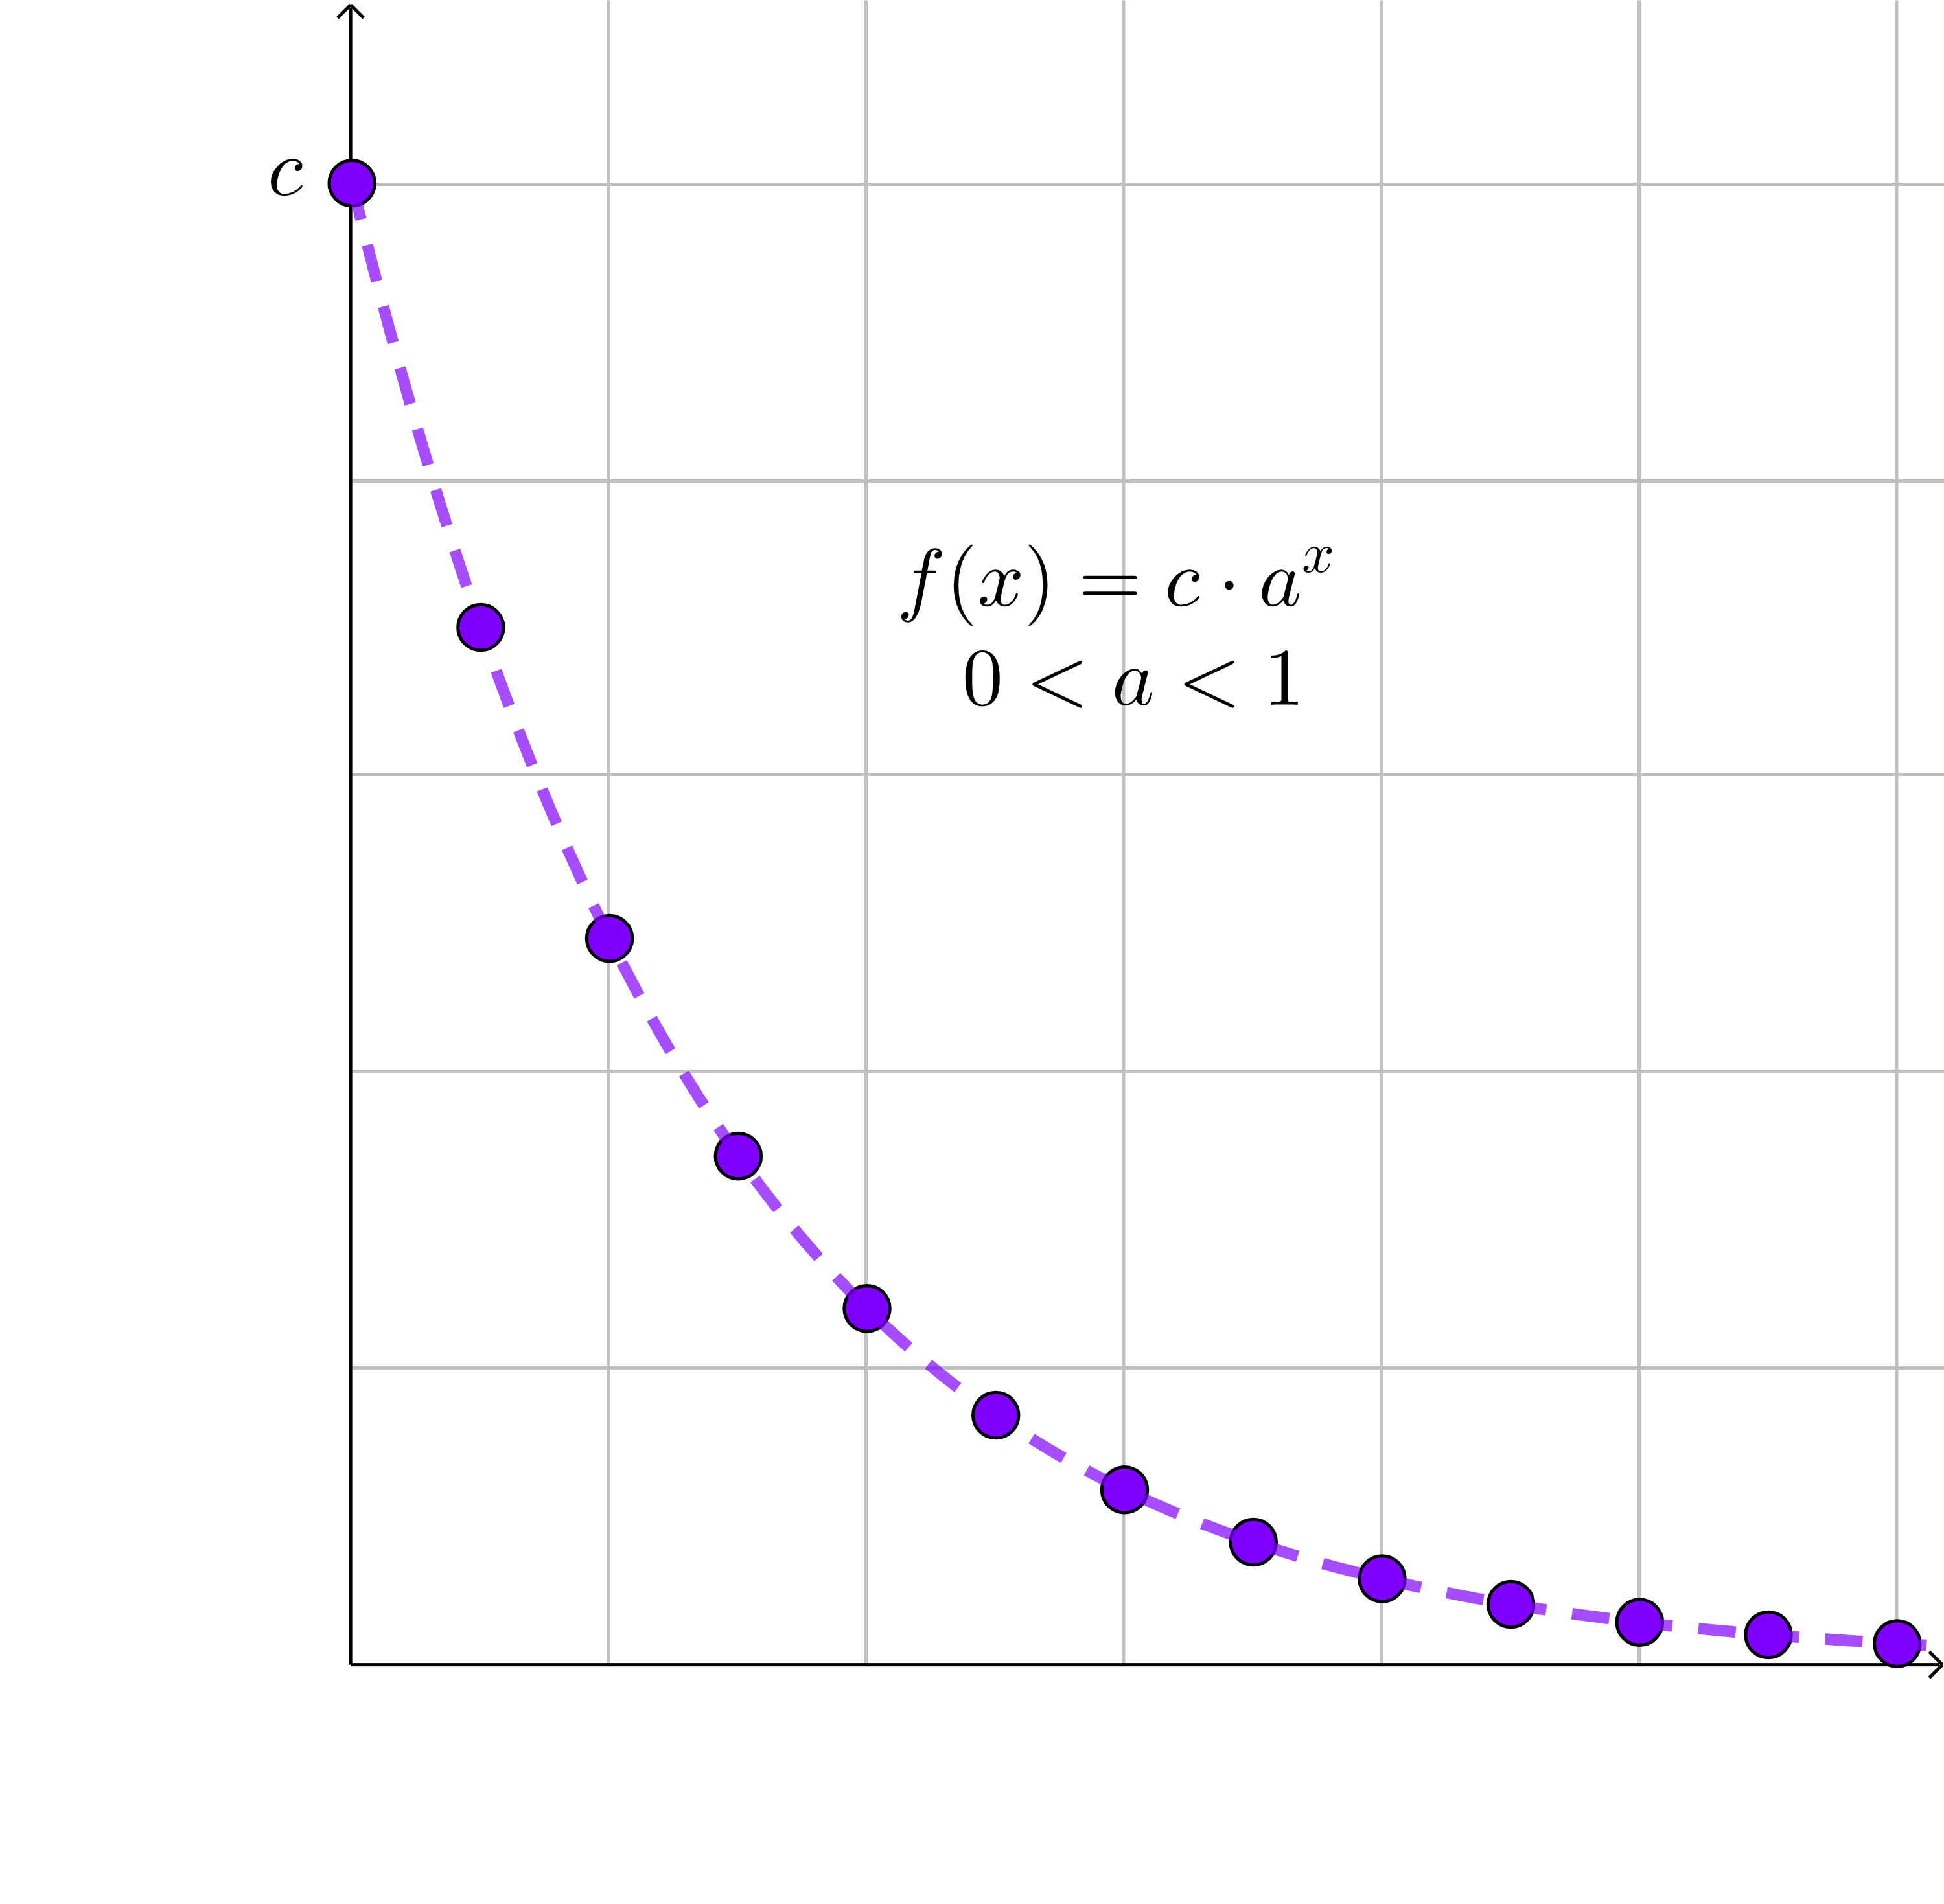
\includegraphics[width=200bp]{exp_decresc.png}
\caption{Crescimento/decrescimento exponenciais.}
\end{figure}

\begin{knowledge}

\begin{itemize}
\item O crescimento exponencial é tão rápido que com poucas multiplicações podemos alcançar valores cujas ordens de grandeza são maiores que a quantidade de átomos estimada para o universo observável (que é algo em torno de $10^{80}$).
\begin{figure}[H]
\centering
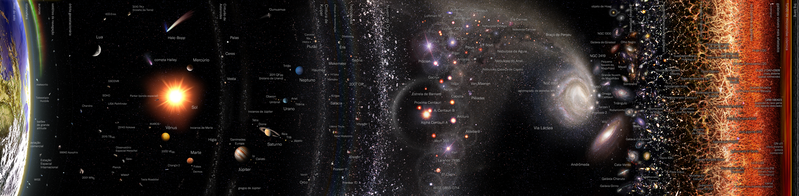
\includegraphics[width=300bp]{universo.png}
\caption{Por Pablo Carlos Budassi - Obra do próprio, CC BY-SA 4.0, \url{https://commons.wikimedia.org/w/index.php?curid=74584500}}
\end{figure}

Você duvida? Vejamos então um exemplo! Pegue uma folha de papel sulfite (ou do seu caderno), cuja espessura é algo em torno de $0{,}075$ milímetros. Se dobramos essa folha ao meio, temos o dobro da espessura inicial, $0{,}15$ milímetros. Dobrando novamente, $0{,}30$ milímetros e assim sucessivamente.

Nenhum ser humano, usando somente as mãos, consegue dobrar uma folha dessas mais que $6$ vezes, pode tentar! Uma folha dobrada $7$ vezes tem a espessura de um caderno de $128$ páginas… E mais, se fosse possível dobrar a folha $23$ vezes, a espessura seria maior que a distância da terra até a Lua.

E aí? Com quantas dobras a espessura alcançaria a ordem de grandeza o número de átomos do universo conhecido? ($267$ dobras)


\item Nesse vídeo, um chef de cozinha chinês faz $128$ noodles em apenas $10$ segundos!
\url{https://youtu.be/S2AnYEheaFM?t=120}

\begin{figure}[H]
\centering
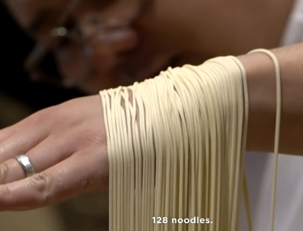
\includegraphics[width=200bp]{noodles.png}
\caption{Imagem extraída do vídeo: \url{https://youtu.be/S2AnYEheaFM?t=120}}
\end{figure}

\item A área de Computação parece desafiar o fato de que não é possível manter um crescimento exponencial por um longo período de tempo devido a escassez de recursos. Talvez o processo exponencial mais longo de que se tem notícia na natureza se refere ao crescimento do poder computacional disponível por $1$ dólar. Este parâmetro seguiu uma exponencial crescente, de constante de tempo de aproximadamente 18 meses, desde o lançamento dos primeiros computadores comerciais em meados da década de 1950 até o início dos anos 2000. Até aquela época, houve uma duplicação do poder computacional disponível por $1$ dólar $27$ vezes seguidas, ou seja, uma variação de $134$ milhões de vezes em 40 anos. Estes números são aproximados pois não conhecemos um estudo preciso nesta direção, nos termos descritos.

\begin{figure}[H]
\centering

\includegraphics[width=250bp]{intel.jpg}
\caption{Foto de Slejven Djurakovic, Unsplash}
\end{figure}

Uma outra lei similar é conhecida como lei de Moore. Gordon Moore foi um dos fundadores da Intel, uma das maiores fabricantes mundiais de circuitos integrados. Ele enunciou a sua lei em 1965, numa época em que um microchip podia integrar algo como 4 transistores: \textbf{``o desempenho de microchips produzidos em massa vai dobrar a cada 18 meses''}. Aqui o limitante de preço é substituído pela condição de produção em massa o que dá um efeito similar, já que só é possível produzir em massa componentes suficientemente baratos para poderem ser absorvidos pelo mercado. Adaptado de \url{https://www.ime.usp.br/~is/infousp/imre/imre.htm}.

\end{itemize}

\end{knowledge}
\clearpage

\def\currentcolor{session2}
\begin{objectives}{A Fazenda de Árvores}
{
	\begin{itemize}
	\item Deduzir uma fórmula para o decaimento exponencial aproximado a partir dos dados de uma tabela;
	\item Fazer previsões a partir da expressão encontrada tanto para o problema direto quanto para o inverso.
	\end{itemize}

	\tcbsubtitle{Cara ou coroa?}

	\begin{itemize}
	\item Reconhecer o padrão de crescimento exponencial que aparece no experimento descrito;
	\item Identificar o fator de crescimento e reconhecer o papel que ele desempenha na situação descrita.

	\end{itemize}

}{1}{2}
\end{objectives}
\begin{sugestions}{A Fazenda de Árvores}
{
	\begin{itemize}
	\item Os dados dessa atividade ficam próximos da exponencial com fator $0{,}95$. Caso seja possível, use ferramentas tecnológicas para análise dos dados.
	\item No item \titem{b)} os valores são pedidos de $5$ em $5$ anos. Verifique se algum estudante percebeu que basta multiplicar $(0,95)^{5}$, e caso positivo peça que ele compartilhe com a turma. Se não, conduza as discussões até essa conclusão.
	\item No item \titem{c)} a pergunta é do tipo problema inverso. Não devemos esperar o uso de logaritmos na solução, mas que o estudante analise os resultados a partir dos dados que ele mesmo gerou no item anterior, fazendo, se necessário, novos cálculos. Algo como: $35$ anos $\rightarrow$ $16,61\%$, $40$ anos $\rightarrow$ $12,85\%$, então os $15\%$ deve estar em algum lugar no meio do caminho, etc.
	\end{itemize}

	\tcbsubtitle{Cara ou coroa?}
	\begin{itemize}
	\item Estimule os estudantes a realizarem o experimento.
	\end{itemize}
}{1}{2}
\end{sugestions}
\begin{answer}{A Fazenda de Árvores}
{

	\begin{enumerate}

	\item{}
	$f(n)=10.000 \times 0,95^{n}$.

	\item{}
	\adjustbox{valign=t}
	{
	\begin{tabu} to \textwidth{|>{\centering}d{.15\textwidth}|*{7}{c|}}
	\hline
	\tcolor{Ano} & 10 & 15 & 20 & 25 & 30 & 35 & 40 \\
	\hline
	\tcolor{Árvores remanescentes} & 5.987 & 4.633 & 3.585 & 2.774 & 2.146 & 1.661 & 1.285 \\
	\hline
	\end{tabu}
	}

	\item{}
	No trigésimo sexto ano.

	\end{enumerate}

	\tcbsubtitle{Cara ou Coroa?}
	\begin{enumerate}

	\item{}
	$\{CC, CK, KC, KK\}$.

	\item{}
	$\{CCC, CCK, CKK, CKC, KKK, KKC, KCK, KCC\}$.

	\item{}
	Deve ser notado que o tamanho do espaço amostral do lançamento de uma moeda $n$ vezes ao ar é dado por $2^{n}$.

	\end{enumerate}
}{0}
\end{answer}
\begin{objectives}{Dobradura}
{
	\begin{itemize}
	\item Reconhecer o padrão de decrescimento exponencial que aparece no experimento descrito;
	\item Identificar o fator de decrescimento e reconhecer o papel que ele desempenha na situação descrita.

	\end{itemize}

	\tcbsubtitle{Duas exponenciais}

	\begin{itemize}
	\item Reconhecer o padrão exponencial em tabelas e gráficos;
	\item Identificar o fator de decrescimento e reconhecer o papel que ele desempenha.
	\end{itemize}
}{1}{1}

\end{objectives}
\marginpar{\vspace{-1.5em}}
\begin{sugestions}{Dobradura}
{
	\begin{itemize}
	\item Estimule os estudantes a realizarem o experimento.
	\end{itemize}

	\tcbsubtitle{Duas exponenciais}

	\begin{itemize}
	\item Havendo disponibilidade utilize uma calculadora gráfica para explorar junto com a turma as características observadas nos gráficos associados a cada uma das expressões.
	\end{itemize}
}{1}{1}
\end{sugestions}
\begin{answer}{Dobradura}
{
	\begin{enumerate}
	\item \adjustbox{valign=t}
	{\setlength\tabulinesep{2.5pt}
	\begin{tabu} to \textwidth{|c|c|c|}
	\hline
	\tcolor{Etapas} & \tcolor{Área de cada região} & \tmcol{1}{c|}{Número de regiões} \\ 
	\hline
	0 & $1$ & $1$ \\ 
	\hline
	1 & $\dfrac{1}{3}$ & $3$ \\ 
	\hline
	2 & $\dfrac{1}{9}$ & $9$ \\ 
	\hline
	3 & $\dfrac{1}{27}$ & $27$ \\ 
	\hline
	4 & $\dfrac{1}{81}$ & $81$ \\ 
	\hline
	5 & $\dfrac{1}{243}$ & $243$ \\ 
	\hline
	\end{tabu}
	}

	\item Em cada nova etapa a área da menor região é obtida dividindo por 3 a área da menor região da etapa anterior, já o número de regiões de uma nova etapa é obtido fazendo a multiplicação de 3 pelo número de regiões da etapa anterior.

	\end{enumerate}
}{1}
\end{answer}
\begin{answer}{Duas exponenciais}
{
	\begin{table}[H]
	\centering

	\begin{tabu} to \textwidth{|>{$}c<{$}|>{$}c<{$}|}
	\hline
	\tnumber
	\bm{x} & \bm{2\cdot3^x} \\
	\hline
	1 & 6 \\
	\hline
	2 & 18 \\
	\hline
	3 & 54 \\
	\hline
	4 & 162 \\
	\hline
	5 & 486 \\
	\hline
	6 & 1458 \\
	\hline
	7 & 4374 \\
	\hline
	8 & 13122 \\
	\hline
	9 & 39366 \\
	\hline
	10 & 118098 \\
	\hline
	\end{tabu}\hspace{1em}
	\begin{tabu} to \textwidth{|>{$}c<{$}|>{$}c<{$}|}
	\hline
	\tnumber
	\bm{x} & \bm{64\cdot(1{,}5)^x} \\
	1 & 96 \\
	\hline
	2 & 144 \\
	\hline
	3 & 216 \\
	\hline
	4 & 324  \\
	\hline
	5 & 486 \\
	\hline
	6 & 729 \\
	\hline
	7 & 1093{,}5 \\
	\hline
	8 & 1640{,}25 \\
	\hline
	9 & 2460{,}375 \\
	\hline
	10 & 3690{,}5625 \\
	\hline
	\end{tabu}
	\end{table}
	\begin{figure}[H]
	\centering
	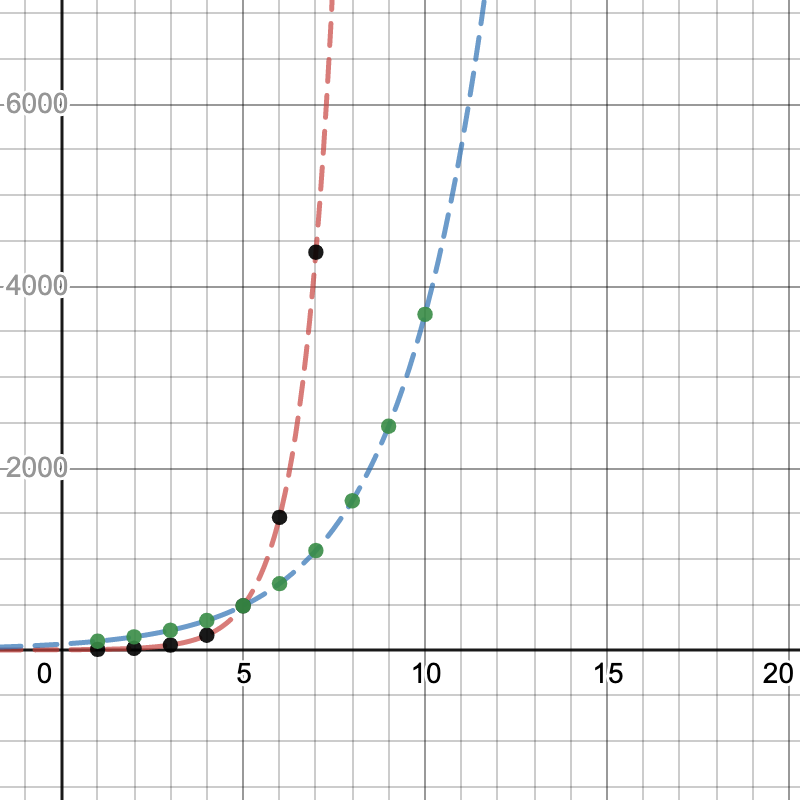
\includegraphics[width=200bp]{Duas_exponenciais.png}
	\end{figure}

	\begin{enumerate}
	\item{}
	$y$ cresce com maior taxa na segunda expressão. As tabelas acima mostram  que os valores correspondentes de $x$ retornam sempre valores de $y$ maiores ou iguais para a segunda expressão.

	\item{}
	$x=5$. Neste ponto os gráficos se interceptam.
	\end{enumerate}
}{9}
\end{answer}
\clearmargin
\begin{sugestions}{Para refletir}
{
	Neste primeiro ``Para Refletir'' do capítulo problematizamos sobre o crescimento exponencial irrestrito, que na maioria das situações se mostra irrealista. Além do crescimento populacional outras situações podem ser utilizadas para ilustrar este fato: crescimento do número de infectados em situações de epidemia (na primeira atividade rapidamente toda a turma foi infectada, depois toda a escola e assim por diante).
	\begin{figure}[H]
	\centering
	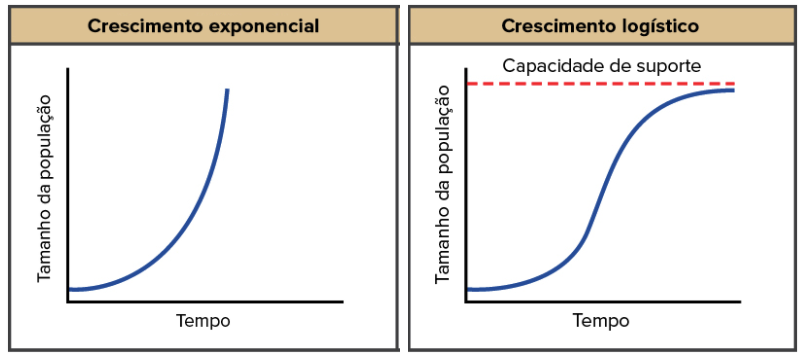
\includegraphics[width=\linewidth]{refletir_logistico.png}
	\end{figure}
	Essas situações são melhores modeladas pelo crescimento logístico, comente sobre o ponto de inflexão, momento em que há uma mudança de comportamento e a curva tende a se aproximar de um limiar, que para o caso de crescimento populacional é chamado capacidade de suporte.
}{1}{2}
\end{sugestions}

\practice{Crescimento e Decaimento exponenciais}

\begin{task}{A Fazenda de Árvores}

Uma fazenda de árvores começou a colher um lote que havia sido plantada anos atrás. A tabela abaixo mostra o número de árvores remanescentes para cada um dos 8 anos de colheita 


\begin{table}[H]
\centering

\begin{tabu} to \textwidth{|d{.15\textwidth}|*{9}{c|}}
\hline
\tcolor{Ano} & 0 & 1 & 2 & 3 & 4 & 5 & 6 & 7 & 8 \\
\hline
\tcolor{Árvores remanescentes} & 10.000 & 9.502 & 9.026 & 8.574 & 8.145 & 7.737 & 7.350 & 6.982 & 6.634 \\
\hline
\end{tabu}
\end{table}

\begin{enumerate}

\item {}
Escreva uma expressão para função que relaciona as árvores remanescentes com o tempo decorrido.

\item{}
Analise os dados da tabela e faça uma previsão para os próximos anos mostrados na tabela a seguir.

\item{}
Os donos da fazenda querem parar a colheita quando sobrarem 15\% do número inicial de árvores do lote. Quando devem parar? 

\end{enumerate}

\begin{table}[H]
\centering

\begin{tabu} to \textwidth{|d{.15\textwidth}|*{7}{>{\centering}m{3em}|}}
\hline
\tcolor{Ano} & 10 & 15 & 20 & 25 & 30 & 35 & 40 \\
\hline
\tcolor{Árvores remanescentes} & & & & & & & \\
\hline
\end{tabu}
\end{table}

\end{task}


\begin{task}{Cara ou Coroa?}

Na teoria das probabilidades, ao analisar as chances de um determinado evento acontecer, é comum considerarmos todas as possibilidades para assim podermos quantificar a probabilidade. O conjunto formado por todas essas possibilidades é chamado de \textbf{espaço amostral}.
Você possui uma moeda, vai girá-la no ar e analisar qual face ficou voltada para cima quando ela cair. O espaço amostral desse experimento contém dois elementos: {cara (C), coroa (K)}. Responda.

\begin{enumerate}

\item{}
Qual o espaço amostral para o experimento de lançar a mesma moeda 2 vezes?

\item{}
E três vezes?

\item{}
Explique a seguinte afirmação:

\textit{“O tamanho do espaço amostral do lançamento de uma moeda várias vezes ao ar aumenta exponencialmente em relação a quantidade de lançamentos”}

\end{enumerate}

\end{task}

\begin{task}{Dobradura}

Uma folha de papel de área 1 é dobrada em três partes iguais, depois em mais três partes iguais, em terços novamente, e assim sucessivamente.

\begin{figure}[H]
\centering
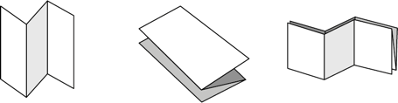
\includegraphics[width=250bp]{dobradura.png}
\end{figure}

\begin{enumerate}

\item{}
Na tabela abaixo registre a área da menor região em cada etapa, e o número total de regiões.

\begin{table}[H]
\centering

\begin{tabular}{|c|c|l|}
\hline
\tcolor{Etapas} & \tcolor{Área de cada região} & \tmcol{1}{c|}{Número de regiões} \\ \hline
0          &      1     & \multicolumn{1}{c|}{1}          \\ \hline
1          &           & \multicolumn{1}{c|}{}    \\ \hline
2          &           &                                 \\ \hline
3          &           &                                 \\ \hline
4          &           &                                 \\ \hline
5          &          &                                 \\ \hline
\end{tabular}
\end{table}

\item{}
Descreva os padrões observados na tabela e encontre uma expressão matemática que sirva para gerá-las em função das etapas.

\end{enumerate}

\end{task}


\begin{task}{Duas exponenciais}

Construa tabelas e gráficos para comparar os valores da variável $y$ nas duas expressões exponenciais para valores inteiros da variável $x$ de $1$ até $10$.

\[
y=2 \cdot 3^{x}  \text{ e } y=64 \cdot (1{,}5)^{x}.
\]

\begin{enumerate}

\item{}
Em qual das duas $y$ cresce a uma taxa maior? Como você sabe?

\item{}
Para que valor de $x$, os valores de $y$ coincidem? Como isso se reflete na representação gráfica?


\end{enumerate}

\end{task}


\begin{reflection}
O crescimento exponencial pressupõe recursos ilimitados e isso faz com que em muitos casos esse tipo de comportamento seja observado apenas em certos períodos de tempo. Isso pode ser visto, por exemplo, na forma como crescem as populações. Com pouco ou sem nenhuma limitação de recursos as populações podem apresentar um crescimento exponencial. No entanto, na prática sabemos que há uma série de limitações - espaço, existência de predadores, escassez de alimentos, etc. - é o que os pesquisadores costumam chamar de \textbf{Resistência Ambiental}. Portanto, após experimentar um período de crescimento exponencial, o que observamos é que a população tende a se estabilizar. Esse comportamento é chamado de \textbf{crescimento logístico}.

\begin{figure}[H]
\centering
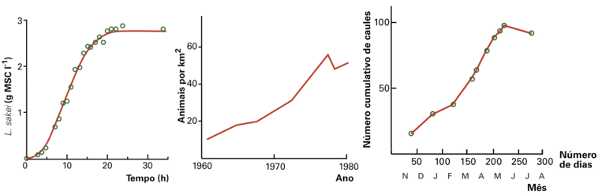
\includegraphics[width=400bp]{logistico.png}
\caption{Exemplos reais de um aumento populacional como descrito acima. (a) a Bactéria Lactobacillus sakei crescendo em um meio de cultura. (b) A população de gnu, na região do Seringueti na Tanzânia. (C) População de juncácea anual , Juncus gerardi.
Fonte: CEPA}
\end{figure}

\end{reflection}
\clearpage
\def\currentcolor{session1}
\begin{texto}
{	\section{Explorando: Variação Percentual}
	Em situações reais é muito comum que a taxa de crescimento seja dada em forma de porcentagem, em que a variação é expressa como fração da quantidade anterior. Nesses casos a variável independente é tomada em intervalos fixos e o foco recai sobre a fração que a variação representa do valor anterior. O caso mais emblemático é o caso dos juros compostos: normalmente se escolhe uma unidade de tempo para a capitalização (meses, anos, trimestres, etc) e se expressa o crescimento/decaimento como uma taxa percentual.

	É importante ressaltar a diferença entre a taxa percentual e a taxa de variação da função. A taxa de variação, como definimos no capítulo sobre Taxa de Variação deste livro, é a razão entre as variações das duas variáveis que estão relacionadas pela função: variação de $y$ por unidades da variável $x$, isto é, $\left( \dfrac{\Delta{y}}{\Delta{x}}\right)$. Para a taxa percentual o $\Delta x$ é fixado e estamos interessados no quociente $\dfrac{y(n+1)-y(n)}{y(n)}$. As atividades aqui nesta seção vão na direção de relacionar a taxa percentual com o fator de crescimento/decaimento. Se uma determinada grandeza cresce (respectivamente diminui) a uma taxa percentual de $20\%$ ao mês, o fator de crescimento (respectivamente decaimento) é o número que multiplicamos o valor atual para obter o valor no próximo mês, a saber $1+0,2$ (respectivamente $1-0,2$). Assim, as funções exponenciais terão a forma $f(x)=c(1+r)^{x}$ (crescimento) ou $f(x)=c(1-r)^{x}$ (decaimento), em que $r$ é a taxa expressa como fração sobre $100$ (ou na forma decimal).

	A primeira atividade do Explorando tem o objetivo de fazer uma breve revisão sobre a ideia de porcentagem. Avalie se é o caso de fazer com a sua turma uma revisão um pouco maior sobre porcentagem.
}
\end{texto}
\begin{objectives}{Tá caro!}
{
	\begin{itemize}
	\item Revisar o conceito de porcentagem.

	\end{itemize}
	\tcbsubtitle{As colônias}

	\begin{itemize}
	\item Reconhecer situações em que uma quantidade aumenta ou diminui a uma taxa percentual constante por unidade da outra.
	\item Expressar o crescimento/decaimento exponencial em termos de variação percentual e vice-versa.
	\end{itemize}
	}{1}{1}
\end{objectives}
\begin{sugestions}{Tá caro!}
{
	\begin{itemize}
	\item Avalie a necessidade de realizar com a turma uma revisão maior sobre porcentagem.
	\end{itemize}

	\tcbsubtitle{As colônias}

	\begin{itemize}
	\item Discuta com os estudantes a possibilidade exibir tabelas e gráficos com valores não necessariamente iguais a 6\% ou 10\% dos valores anteriores, mas que possam ser aproximados tentando retratar alguma coleta de dados real e que tenha levado os cientistas a escolher o modelo exponencial.
	\item No item (g), se achar conveniente, apresente as expressões $(1+r)$ para crescimento e $(1-r)$ para decaimento, nas quais a taxa percentual $r$ é sempre considerada um número positivo.
	\end{itemize}
}{0}{0}
\end{sugestions}
\begin{answer}{Tá caro!}
{
	\begin{enumerate}[itemsep=0pt]

	\item{}
	Aumento de $R\$ 80,00$, que representa $50\%$ do valor original do tênis.

	\item{}
	$R\$ 176,00$.

	\item{}
	Narrativa apresentando um produto ou serviço cujo valor seja maior ou igual a $R\$ 800,00$.

	\end{enumerate}

	\tcbsubtitle{As colônias}

	\begin{enumerate}
	
	\item{}
	Os valores abaixo não são a única resposta correta, e podem variar dependendo da maneira como se procede os cálculos.

	\begin{table}[H]
	\centering
	
	\begin{tabu} to \textwidth{|>{$}c<{$}|>{$}c<{$}|}
	\hline
	\tnumber
	\bm{t}\text{ \textbf{(meses)}} & \bm{C}\text{ \textbf{coelhos}} \\
	\hline
	0 & 100 \\
	\hline
	1 & 106 \\
	\hline
	2 & 112 \\
	\hline
	3 & 119 \\
	\hline
	4 & 126 \\
	\hline
	5 & 133 \\
	\hline 
	6 & 141 \\
	\hline
	7 & 150 \\
	\hline
	8 & 159 \\
	\hline
	9 & 169 \\
	\hline
	10 & 179 \\
	\hline
	11 & 190 \\
	\hline
	12 & 201 \\
	\hline
	\end{tabu}
	\hspace{1em}	
	\begin{tabu} to \textwidth{|>{$}c<{$}|>{$}c<{$}|}
	\hline
	\tnumber
	\bm{t}\text{ \textbf{(meses)}} & \bm{B}\text{ \textbf{bactérias}} \\
	\hline
	0 & 950.000 \\
	\hline
	1 & 855.000 \\
	\hline
	2 & 769.500 \\
	\hline
	3 & 692.550 \\
	\hline
	4 & 623.295 \\
	\hline 
	5 & 560.965 \\
	\hline
	6 & 504.868 \\
	\hline
	7 & 454.382 \\
	\hline
	8 & 408.943 \\
	\hline
	9 & 368.049 \\
	\hline
	10 & 331.244 \\
	\hline
	11 & 298.120 \\
	\hline
	12 & 268.308 \\
	\hline
	\end{tabu}
	\end{table}

	\item{}
	$100+6\%100 = 106$, $106+6\%106=112$, e assim sucessivamente.

	$950.000-10\%950.000 = 855.000$, $855.000-10\%855.000 = 769.500$, e assim sucessivamente. 

	\item{}
	Sim. Basta fazer as divisões de cada valor pelo anterior e observar que os valores ficam próximos de constantes, em cada caso: $1,06$ no primeiro caso e $0,9$ no segundo caso.

	\item{}
	O fator será dado por $1$ mais a taxa percentual considerada positiva no caso de crescimento ($1+6\%$) e negativa para o decaimento ($1-10\%$).

	\item{}
	$C(t)=100\cdot1,06^{t}$, e $B(t)=950.000\cdot0,9^t$.

	\item{}
	---
	\item{}
	$P(t)=P_0\cdot(1+r)^t$.

	\end{enumerate}
}{9}
\end{answer}
\clearmargin
\begin{objectives}{Juros}
{
\begin{itemize}
\item Investigar o crescimento de uma movimentação financeira com uma dada taxa de capitalização composta. Relacionar taxa percentual $r$ e fator de crescimento $(1+r)$ / decaimento $(1 - r)$.
\end{itemize}
}{1}{2}
\end{objectives}
\begin{sugestions}{Juros}
{
\begin{itemize}
\item Reforce com os estudantes a relação entre a taxa percentual e o fator de multiplicação. 
\end{itemize}
}{1}{2}
\end{sugestions}
\begin{answer}{Juros}
{
\begin{enumerate}

\item{}
$100(1+r)^2 =110,25 \iff r=0,05 = 5\%$ 

\item{}
$100(1+0,05)=105$

\item{}
$100(1+0,05)^3=115,76$

\end{enumerate}
}{1}
\end{answer}

\explore{Variação percentual}

\begin{task}{Tá caro!}

Você está precisando comprar um tênis novo e vem pesquisando os preços. Na sua última consulta o modelo que você deseja estava custando $160$ reais. Ao fazer uma nova consulta, você verifica que agora ele custa $240$ reais, e resolve não comprar até o preço baixar um pouco.

\begin{enumerate}

\item{}
Qual foi o valor do aumento de preço observado e que valor ele representa em termos percentuais? Explique seu cálculo.

\item{}
Levando em consideração que houve um aumento geral nos preços, você estava esperando um aumento de no máximo $10\%$ no valor do tênis. Que valor máximo deveria estar custando o tênis para que você o comprasse.

\item{}
Construa uma narrativa de outra situação em que o mesmo aumento de preço de $80$ reais esteja dentro da margem de $10\%$ esperada.

\end{enumerate}

\end{task}

\begin{task}{As colônias}

Analise cada uma das situações abaixo e em seguida responda as perguntas para cada uma delas.

 \textbf{(A)} Uma população de 100 coelhos é introduzida em uma reserva ecológica. Após um período de observação de 12 meses, os biólogos concluíram que essa colônia cresceu ao longo do ano seguindo uma taxa percentual aproximada de $6\%$ ao mês, isto é, a cada mês a população de coelhos na colônia estava aproximadamente $6\%$ maior em relação ao registro do mês anterior.


 \textbf{(B)} Um laboratório está pesquisando a eficácia de um antibiótico e uma equipe de biomédicos o adiciona em uma colônia de bactérias com uma população de $950.000$ indivíduos. As células então começam a morrer de maneira que ao final de 12 horas, os pesquisadores afirmam que população da colônia diminuiu a uma taxa percentual de $10\%$ a cada hora.

\begin{enumerate}
%\item{}
%Elabore uma tabela e um gráfico com os possíveis dados observados por eles.
%
%\item{}
%Para a situação (A) qual a taxa percentual de crescimento do início até o terceiro período de tempo? E entre o terceiro e o sexto períodos? Por que não são iguais ao triplo da taxa percentual para um período?
%
%\item{}
%Para a situação (B) qual dos modelos a seguir melhor descreveria os dados?
%
%(    ) linear \quad (    ) exponencial.
%
%Explique sua escolha.
%
%\item{}
%No caso do crescimento exponencial, qual a relação do fator de crescimento/decaimento com a taxa percentual?
%
%\item{}
%Escreva uma expressão matemática para cada uma das situações que relacione o números de indivíduos nas colônias com o número de meses (ou horas) decorridos desde o início das observações.
%
%\item{}
%Denotando por $C$ o valor inicial e por $r$ a taxa percentual observada, generalize as expressões obtidas no item anterior.

\item{}
Elabore uma tabela com os possíveis dados observados pelos pesquisadores em cada uma das situações.
\item{}
Descreva como você obteve os dados das tabelas anteriores.
\item{}
Pode-se afirmar que os dados tabelas apresentam crescimento e decaimento exponenciais? Em caso afirmativo, quais são os fatores em cada situação?
\item{}
Qual a relação do fator de crescimento/decaimento com a taxa percentual?
\item{}
Escreva uma expressão matemática para cada uma das situações que relacione o números de indivíduos nas colônias com o número de meses (ou horas) decorridos desde o início das observações.
\item{}
Com a ajuda de uma calculadora compare os valores gerados pela expressão matemática com as que você calculou no item \titem{a)}.
\item{}
Denotando por $P(t)$ a população no tempo $t$, $P_0$ seu valor inicial e $r$ a taxa percentual observada, generalize as expressões obtidas no item anterior.
\end{enumerate}

\end{task}

%\begin{table}[]
%	\begin{tabular}{|c|c|c|c|c|c|c|c|c|c|c|c|c|c|}
%		\hline
%		t (meses)   & 0   & 1   & 2   & 3   & 4   & 5   & 6   & 7   & 8   & 9   & 10  & 11  & 12  \\ \hline
%		C (coelhos) & 100 & 106 & 112 & 119 & 126 & 133 & 141 & 150 & 159 & 169 & 179 & 190 & 201 \\ \hline
%	\end{tabular}
%\end{table}




\begin{task}{Juros}


Você acabou de adquirir um produto de R\$ $200$ e o pagamento proposto pela loja é da seguinte maneira: uma entrada de R\$ $100$ paga no ato da compra e mais uma parcela de  R\$ $110{,}25$ após 2 meses.

\begin{enumerate}

\item{}
Considerando que a taxa percentual mensal de acréscimo será a mesma nos dois meses, qual é o valor dessa taxa na transação proposta?

\item{}
Com base na taxa percentual que você encontrou no item anterior, que valor deveria ser pago se a segunda parcela fosse apenas $1$ mês depois da compra?

\item{}
E se a segunda parcela fosse paga com $3$ meses de intervalo, qual seria o valor a pagar? 

\end{enumerate}

\end{task}

\arrange{Variação Percentual}

Em diversas situações as variações das quantidades no tempo são expressas em termos percentuais: o preço da gasolina subiu $10\%$, o número de desempregados aumentou $50\%$, o PIB do Brasil encolheu $2{,}5$\%, o número de pessoas infectadas pelo vírus aumentou $300\%$, etc. Isso geralmente ocorre quando se quer evidenciar que fração do último registro aquela variação representa. Dizer que o número de infectados por um vírus aumentou $300\%$ significa que se a quantidade de infectados era $I_{0}$ e passou a ser $I_{1}$, então

\[
\dfrac{I_{1}-I_{0}}{I_{0}}=300\% \iff I_{1}-I_{0}=3I_{0} \iff I_{1}=4I_{0}.
\]

De maneira mais geral, se a taxa percentual é r(sendo positiva para crescimento e negativa para redução), então temos

\[
\dfrac{I_{1}-I_{0}}{I_{0}}=r \iff I_{1}-I_{0}=rI_{0} \iff I_{1}=I_{0}+rI{0} \iff I_{1}=(1+r)I_{0}.
\]

Quando é o caso de que taxa percentual observada permanece constante ao longo de um intervalo de tempo, então estamos diante de uma situação de crescimento (taxa positiva) ou decaimento (taxa negativa) exponencial.

Mais ainda, como pudemos observar acima, uma variação com taxa percentual $r$ corresponde a um fator de crescimento/decaimento $1+r$, isto é, para saber o valor atual de uma determinada grandeza que aumentou segundo uma taxa percentual $r$, basta multiplicar o seu último registro por $1+r$.

\begin{center}
\begin{tabular}{|c|c|}
\hline
\tmcol{2}{|c|}{Taxa percentual: $\bm{r}$} \\ \hline
$t=0  $       & $C$ (valor inicial)          \\ \hline
$t=1$         & $C(1+r)$                     \\ \hline
$t=2$         & $C(1+r)(1+r)=C(1+r)^{2} $       \\ \hline
$t=3$         & $C(1+r)^{2}(1+r)=C(1+r)^{3} $        \\ \hline
$\cdots$         & $\cdots$                       \\ \hline
$t=n$         & $C(1+r)^{n-1}(1+r)=C(1+r)^{n}$        \\ \hline
\end{tabular}
\end{center}

No contexto das transações financeiras o acréscimo no valor do dinheiro (dívida, investimento, crédito, débito, etc) é chamado de \textbf{juro} e a taxa percentual de variação segundo a qual calculamos o juro chama-se \textbf{taxa de juros}. Esse sistema em que o juro é calculado sobre o valor imediatamente anterior é conhecido como \textbf{capitalização composta} (também chamado de juro sobre juro) e é adotado na maior parte das transações financeiras do mundo.

O valor de um investimento de R\$ 1.000 a uma taxa de juros de 10\% ao mês evolui exponencialmente da seguinte maneira:

\begin{table}[H]
\centering
\setlength\tabulinesep{2.5pt}

\begin{tabu} to \textwidth{|c|c|c|}
\hline
\tcolor{Tempo} & \tcolor{Valor}                       & \tcolor{Juro}                \\ \hline
$t=0$   & R\$ $1.000$ (capital inicial) & R\$ 0               \\ \hline
$t=1$   & R\$ $1.000(1+0{,}1)$ = R\$ $1.100$   & R\$ $100$             \\ \hline
$t=2$   & R\$ $1.100(1+0{,}1)$ = R\$ $1.210$   & R\$ $110$             \\ \hline
$t=3$   & R\$ $1.210(1+0{,}1)$ = R\$ $1.331$   & R\$ $121$             \\ \hline
      &                             &                     \\ \hline
$t=n$   & $R\$1000\cdot (1{,}1)^{n}$               & $R\$ 1000\cdot (1{,}1)^{n-1} \cdot 0,1$ \\ \hline
\end{tabu}
\end{table}

\begin{figure}[H]
\centering
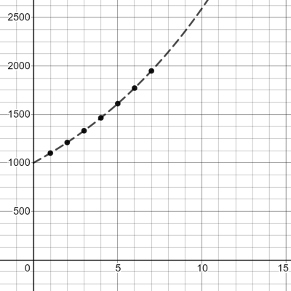
\includegraphics[width=150bp]{juros.png}
\caption{Evolução do valor de um investimento de R\$ 1000,00 capitalizado a uma taxa de juros de 10\% ao mês.}
\end{figure}

\needspace{.2\textheight}

\def\currentcolor{session2}
\begin{objectives}{Antílopes}
{
\begin{itemize}
\item Comparar o crescimento exponencial e o crescimento de variação linear por meio de tabelas.
\end{itemize}

\tcbsubtitle{Fatores e taxas}

\begin{itemize}
\item Identificar, a partir da expressão exponencial seus principais elementos e reconhecer nela o crescimento ou decaimento.

\item Esboçar gráficos de exponenciais discretas.
\end{itemize}

}{1}{2}
\end{objectives}
\begin{sugestions}{Antílopes}
{
\begin{itemize}
\item Atividade retirada de \textit{Sawalha, Yamamah, "The Effects Of Teaching Exponential Functions Using Authentic Problem Solving On Students’ Achievement
And Attitude" (2018).Wayne State University Dissertations. 1959.}
\url{https://digitalcommons.wayne.edu/oa_dissertations/1959}

\item Para identificar os crescimentos exponenciais é necessário fazer alguns arredondamentos. A ideia é que o estudante identifique as tabelas que mais se aproximam dos modelos teóricos.
\end{itemize}

\tcbsubtitle{Fatores e taxas}
\begin{itemize}
\item Até esse momento estamos considerando apenas domínio natural, portanto os gráficos deverão ser esboçados apenas com pontos.

\item Estimule os estudantes a escrever a variação percentual na representação decimal e com o símbolo de porcentagem.

\end{itemize}

}{1}{2}
\end{sugestions}
\begin{answer}{Antílopes}
{

\begin{enumerate}

\item{}
Tabela $1$.

\item{}
Tabela $2$.

\item{}
$0,3\%$ ao ano ou $3$ antílopes por ano.

\item{}
Tabela $1$ é exponencial com fator $1,03$, tabela $2$ tem variação linear com taxa variação $30$ antílopes. A tabela $3$ pode ser considerada exponencial com fator $1,003$ ou linear com taxa de variação $3$ antílopes.

\end{enumerate}

\vspace{-.5em}

\tcbsubtitle{Fatores e taxas}

\begin{table}[H]
\centering
\setlength\tabulinesep{3.5pt}

\begin{tabu} to \linewidth{|c|c|c|>{\centering}m{.2\linewidth}|>{\centering}d{.2\textwidth}|}
\hline
\thead
Valor inicial & Fator & Taxa percentual & Crescimento ou decaimento? & Esboço do gráfico 
\tabularnewline 
\hline
$3$ & $1{,}7$ & $0{,}7=70\%$ & Crescimento & 

%Figura 1

\adjustbox{valign=c}
{
\resizebox{.2\textwidth}{!}
{
\begin{tikzpicture}[scale=1/3]
\draw [thick] (0,6cm) -- (0,0) -- (6cm,0);
\draw [domain=0:1.3, densely dashed, \currentcolor!80] 
plot (\x,{3*(1.7)^(\x)}) 

node at (0,3) [fill, circle, inner sep=1pt, label=left:{$3$}, overlay] {}; 
\end{tikzpicture}
}
}

\tabularnewline 
\hline
$10$ & $0{,}2$ & $-0{,}8=-80\%$ & Decaimento & 

%Figura 2

\adjustbox{valign=c}
{
\resizebox{.2\textwidth}{!}
{
\begin{tikzpicture}[scale=1/5]
\draw [thick] (0,11cm) -- (0,0) -- (11cm,0);
\draw [very thick, domain=0:11, densely dashed, \currentcolor!80] 
plot (\x,{10*(0.2)^(\x)}) 

node at (0,10) [fill, circle, inner sep=1pt, label=left:{$10$}, overlay] {}; 
\end{tikzpicture}
}
}

\tabularnewline 
\hline
$2$ & $0{,}5$ & $-0{,}5=-50\%$ & Decaimento & 

%Figura 3

\adjustbox{valign=c}
{
\resizebox{.2\textwidth}{!}
{
\begin{tikzpicture}[scale=1/2]
\draw [thick] (0,5cm) -- (0,0) -- (5cm,0);
\draw [very thick, domain=0:5, \currentcolor!80, densely dashed] 
plot (\x,{2*(1/2)^(\x)}) 

node at (0,2) [fill, circle, inner sep=1pt, label=left:{$2$}, overlay] {};
\end{tikzpicture}
}
}

\tabularnewline 
\hline
$5$ & $3$ & $2=200\%$ & Crescimento & 

%Figura 4

\adjustbox{valign=c}
{
\resizebox{.2\textwidth}{!}
{
\begin{tikzpicture}[scale=1/5]
\draw [thick] (0,11cm) -- (0,0) -- (11cm,0);
\draw [very thick, domain=0:.715, densely dashed,\currentcolor!80] 
plot (\x,{5*(3)^(\x)}) 

node at (0,5) [fill, circle, inner sep=1pt, label=left:{$5$}, overlay] {}; 
\end{tikzpicture}
}
}

\tabularnewline 
\hline
$0{,}2$ & $7$ & $6=600\%$ & Crescimento & 

%Figura 5

\adjustbox{valign=c}
{
\resizebox{.2\textwidth}{!}
{
\begin{tikzpicture}[scale=1/2]
\draw [thick] (0,5cm) -- (0,0) -- (5cm,0);
\draw [very thick, domain=0:1.65, densely dashed,\currentcolor!80] 
plot (\x,{0.2*(7)^(\x)}) 

node at (0,.2) [fill, circle, inner sep=1pt, label=left:{$0{,}2$}, overlay] {};  
\end{tikzpicture}
}
}

\tabularnewline 
\hline
\end{tabu}
\end{table}
}{0}
\end{answer}
\clearmargin
\begin{objectives}{Juros sobre juros}
{
\begin{itemize}
\item Praticar em situações concretas os conceitos de juro, taxa e período. 
\end{itemize}
}{1}{1}
\end{objectives}
\begin{sugestions}{Juros sobre juros}
{
\begin{itemize}
\item A ideia aqui não é fazer uma exposição exaustiva sobre juros compostos, mas sim se apoiar nas ideias construídas até aqui para resolver os problemas propostos.

\item  Sugerimos dividir a turma em duplas/trios para a resolução dos problemas e posterior apresentação para os colegas. Caso julgue necessário aumente a lista de problemas para deixar a atividade mais interessante.

\end{itemize}
}{1}{1}
\end{sugestions}
\begin{answer}{Juros sobre juros}
{
\begin{enumerate}

\item{}
$\dfrac{27.500}{1{,}017^{12}}=22.463{,}70$

\item{}
$40.000(1+r)^4=43.894{,}63 \iff r=0,0235=2{,}35\%$

\item
$88.000(1{,}045)^5-88.000=21.664{,}01$

\item
$(1{,}099)^2=1{,}2078$, portanto geram o mesmo valor.

\end{enumerate}
}{1}
\end{answer}
\practice{Variação percentual}

\begin{task}{Antílopes}

As tabelas abaixo mostram os dados de três possíveis variações nas populações de antílopes em uma reserva. Baseando-se nos dados, responda às questões a seguir.
\begin{multicols}{3}

\begin{table}[H]
\centering

\begin{tabu} to \textwidth{|c|c|}
\hline
\thead
Ano & Antílopes \\
\hline
2017 & $1.000$ \\
\hline
2018 & $1.030$ \\
\hline
2019 & $1.061$ \\
\hline
2020 & $1.093$ \\
\hline
\end{tabu}

\caption*{Tabela 1}
\end{table}

\begin{table}[H]
\centering

\begin{tabu} to \textwidth{|c|c|}
\hline
\thead
Ano & Antílopes \\
\hline
2017 & $1.000$ \\
\hline
2018 & $1.030$ \\
\hline
2019 & $1.060$ \\
\hline
2020 & $1.090$ \\
\hline
\end{tabu}

\caption*{Tabela 2}
\end{table}


\begin{table}[H]
\centering

\begin{tabu} to \textwidth{|c|c|}
\hline
\thead
Ano & Antílopes \\
\hline
2017 & $1.000$ \\
\hline
2018 & $1.003$ \\
\hline
2019 & $1.006$ \\
\hline
2020 & $1.009$ \\
\hline
\end{tabu}

\caption*{Tabela 3}
\end{table}
\end{multicols}



\begin{enumerate}

\item{}
Que tabela mostra a população de antílopes crescendo a uma taxa de 3\% ao ano?

\item{}
Que tabela mostra a população de antílopes crescendo a uma taxa de 30 antílopes por ano?

\item{}
Descreva o crescimento da tabela remanescente.

\item{}
Alguma dessas variações é linear? E exponencial? Explique.

\end{enumerate}

\end{task}

\begin{task}{Fatores e taxas}

Classifique dentre os modelos dados abaixo os que apresentam crescimento exponencial ou decaimento exponencial. Identifique o que se pede nas colunas da tabela.

\begin{table}[H]
\centering

\begin{tabu} to \textwidth{|>{\centering}m{.2\textwidth}|c|c|>{\centering}m{.1\textwidth}|>{\centering}m{.2\textwidth}|>{\centering}m{.15\textwidth}|}
\hline
\thead
Modelo & Valor inicial & Fator & Taxa percentual & Crescimento ou decaimento? & Esboço do gráfico 
\tabularnewline 
\hline
$y(z)=3(1{,}7)^{z}$ & & & & & \tikz\draw [<->] (0,1cm) -- (0,0) -- (1cm,0); 
\tabularnewline 
\hline
$p(r)=10(0{,}2)^{r}$ & & & &  & \tikz\draw [<->] (0,1cm) -- (0,0) -- (1cm,0); 
\tabularnewline 
\hline
$s(t)=2\cdot \left(\dfrac{1}{2}\right)^{t}$ & & & & & \tikz\draw [<->] (0,1cm) -- (0,0) -- (1cm,0); 
\tabularnewline 
\hline
$M(x)=5\cdot 3^{x}$ & & & & & \tikz\draw [<->] (0,1cm) -- (0,0) -- (1cm,0); 
\tabularnewline 
\hline
$F(y)=0,2\cdot 7^{y} $ & & & & & \tikz\draw [<->] (0,1cm) -- (0,0) -- (1cm,0); 
\tabularnewline 
\hline
\end{tabu}
\end{table}


\end{task}
% 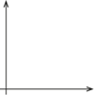
\includegraphics[scale=0.25]{grafico1.png}

\begin{task}{Juros sobre juros}

Resolva os seguintes problemas:

\begin{enumerate}

\item{}
Se uma pessoa deseja obter R\$ $27.500{,}00$ em um ano, quanto deverá depositar hoje em uma alternativa de poupança que rende $1{,}7\%$ de juros compostos ao mês?

\item{}
Qual a taxa percentual mensal de juros de uma aplicação de R\$ $40.000{,}00$ que produz um total de R\$ $43.894{,}63$ ao final de um quadrimestre.

\item{}
Determinar o juro total a ser pago em um empréstimo de R\$ $88.000{,}00$ pelo prazo de $5$ meses à taxa composta de $4{,}5\%$ ao mês.

\item{}
Qual das opções gera um valor maior ao final de 1 ano: aplicar um capital de $R\$60.000{,}00$ à taxa de juros de $9{,}9\%$ ao semestre ou à taxa de $20{,}78\%$ ao ano.

\end{enumerate}

\end{task}

\begin{paginatexto}
\section{Explorando: Propriedades Aritméticas}

Até esse momento espera-se que o estudante tenha o entendimento da exponenciação como processo (e não apenas somente como ação de multiplicações repetidas), enxergando $2^{3}$ como um produto de três fatores $2$, sem ter que necessariamente ``fazer a conta'', ou ainda como uma função de domínio discreto (finito ou enumerável). O objetivo dessa seção é avançar na direção de dar sentido aos expoentes não naturais: negativos, racionais e irracionais, e com isso entender a função exponencial definida para todo o conjunto dos números reais. 

Em geral, os livros-texto de matemática apoiam-se no fato de o estudante ter aprendido as operações com potências durante o Ensino Fundamental (incluindo operações e propriedades operatórias envolvendo expoentes negativos e racionais) e a partir daí constroem a função exponencial de domínio real. Não é raro, entretanto, muitas vezes devido à abordagem tecnicista e mecânica que se dá ao tema, que os estudantes não se recordem ou mesmo que confundam as propriedades, sem saber o que devem fazer com os expoentes em cada caso (BORGES et al, 2015). Dessa forma, escolhemos aqui percorrer novamente esse caminho, sem necessariamente gastar muito tempo com as propriedades mecânicas, mas com a intenção de redirecionar o foco e trazer significados para as definições. 

O estudante deve em algum momento dar sentido ao ``produto de x fatores a'' quando $x$ não é um número inteiro positivo. Responder a perguntas do tipo: o quanto cresce uma planta em um dia, considerando que sua altura dobra de medida a cada semana? E em meia semana, um décimo de semana, e a duas semanas atrás etc? A chave para responder a esses questionamentos está na ideia de fator de crescimento. Por exemplo, para as frações, se a altura da planta duplica em uma semana, uma semana atrás a altura era a metade do que é hoje; em meia semana adiante ela vai ser multiplicada por um outro fator $k$ de maneira que $k \times k=2$, ou seja, $k= \sqrt{2}$ . Por outro lado, como se trata da função $f(t)=2^{t}$, temos $k=f\left( \dfrac{1}{2} \right)$ o que nos leva (e dá sentido) à igualdade $2^{1/2}=\sqrt{2}$.

\resizebox{\linewidth}{!}
{
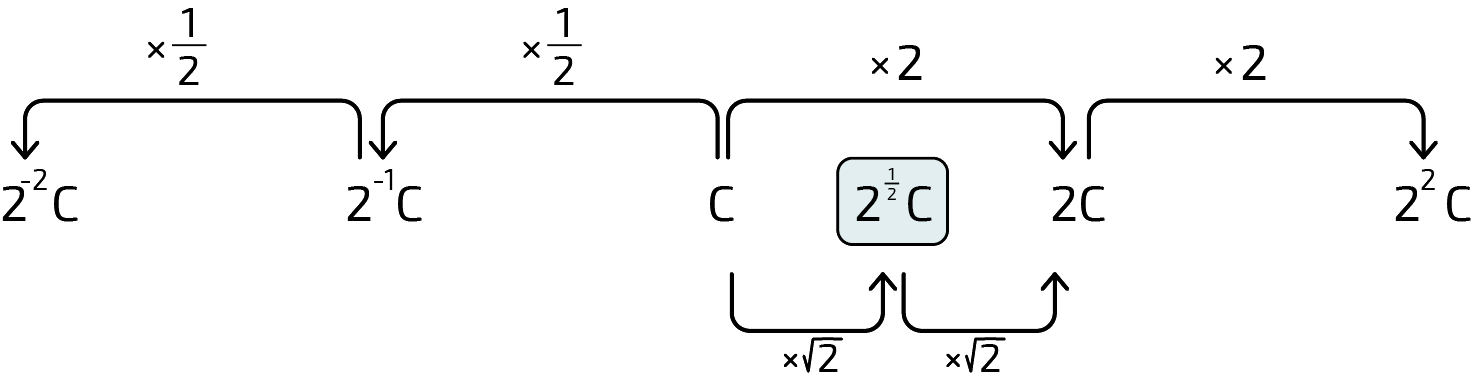
\includegraphics[width=350bp]{exp_racional.png}
}

É claro que há sutilezas aqui, estamos falando de um processo de limite que envolve uma função contínua. Mais importante do que saber calcular (por aproximação) uma potência com expoente racional é olhar para ele como um número real que existe e está bem definido. Ou seja, superar a ideia de ter que ``fazer a conta'' para entendê-lo como um objeto matemático com características e potencial aritméticos.

A abordagem que adotamos nesta seção está baseada em um conjunto de quatro níveis sucessivos que os estudantes devem percorrer enquanto aprendem funções exponenciais. Eles foram propostos por \citep{Weber2002}) com base na teoria APOS (ação - processo - objeto - esquema) de Dubinsky. Estes quatro níveis (do mais básico para o mais avançado) são:

\begin{enumerate}[label=\titem{\arabic*.}]
\item  Uma compreensão de \textbf{ação} dos expoentes (calcular $b^{x}$ envolve multiplicar repetidamente por $b$ um número $x$ de vezes).
\item  Uma compreensão de \textbf{processo} dos expoentes. Um entendimento do processo surge quando um aluno repete uma ação e reflete sobre ela. Segundo Weber (2002), um aluno com um entendimento de processo pode imaginar o resultado da exponenciação sem realmente executar o cálculo. Ele pode raciocinar sobre as propriedades da função exponencial e pode reverter a exponenciação para obter logaritmos; o domínio é restrito aos números naturais.

\item  \textbf{Expressões exponenciais} a partir de um processo. Neste nível, uma expressão exponencial representa o resultado da exponenciação. O número $2^{3}$ pode ser percebido de dois modos: como um comando externo para multiplicar o número dois por ele mesmo três vezes, ou pode ser percebido como um objeto matemático, representado o resultado da exponenciação.

\item  Uma compreensão \textbf{generalizada} dos expoentes. Neste nível, o estudante pode interpretar situações nas quais o domínio da função exponencial não está restrito ao conjunto dos números naturais.
\end{enumerate}
\end{paginatexto}
\def\currentcolor{session1}
\begin{objectives}{Expoentes inteiros}
{
\begin{itemize}
\item Revisar as propriedades aritméticas das potências com expoentes inteiros;
\item Construir de modo intuitivo o significado de potências com expoentes inteiros negativos;

\end{itemize}
}{1}{1}
\end{objectives}
\begin{sugestions}{Expoentes inteiros}
{
\begin{itemize}

\item Esta atividade tem um grande potencial para ser aplicada na forma de investigação. Separe a turma em grupos de no máximo $4$ alunos e peça que analisem os cartões em busca de relações e padrões, sem deixar que vejam as perguntas seguintes. Como se trata de um assunto supostamente conhecido por eles desde o Ensino Fundamental, espera-se que consigam perceber algumas relações importantes. Procure provocá-los com perguntas que levem-nos às propriedades das potências. Ao final, peça que socializem com os demais colegas as suas descobertas;

\item Espera-se que aqui ele solidifique a ideia de potência como produto de fatores repetidos, mas que perceba que não necessariamente ele precisa saber o resultado dessa operação para trabalhar com os objetos. Por outro lado, espera-se que ele extrapole essa ideia de multiplicação repetida ao lidar com expoentes negativos;

\item Chame a atenção dos estudantes para o fato de que ao lidar com expoentes negativos ampliamos a noção de potência de forma que a multiplicação repetida não é mais “a regra” ou a maneira correta de enxergar, ou seja, que $2^{-3}$ não é $2$ multiplicado por si mesmo $-3$ vezes. E que essa ampliação é feita de maneira que preserva as propriedades aritméticas já conhecidas.

\end{itemize}
}{1}{1}
\end{sugestions}
\begin{answer}{Expoentes inteiros}
{
\begin{enumerate}
\item
O número $2$ elevado ao número em cinza é igual ao número em vermelho.

\end{enumerate}
}{1}
\end{answer}
\clearmargin
\marginpar{\vspace{.5em}}
\begin{answer}{Expoentes inteiros}
{
\begin{enumerate}\setcounter{enumi}{1}

\item
Quando nos movemos de um cartão para o cartão seguinte a direita observamos que o número em vermelho é multiplicado por $2$ e o número em cinza aumenta uma unidade.

\begin{figure}[H]
\centering
\noindent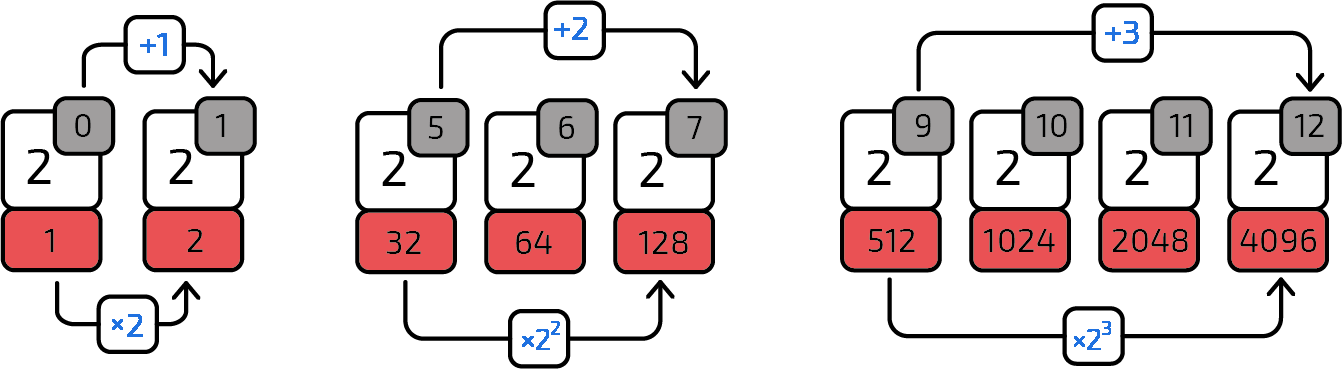
\includegraphics[width=\linewidth]{resp_inteiros_b.png}
\end{figure}

\item
O esquema será:

\begin{figure}[H]
\centering
\noindent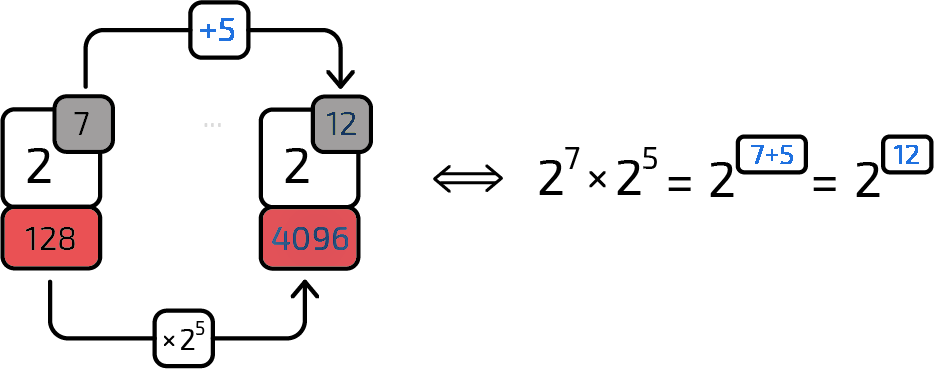
\includegraphics[width=.75\linewidth]{resp_inteiros_c.png}
\end{figure}

Alguns outros exemplos: $2^{9} \times 2^{4} =2^{9+4}=2^{13}$,\quad $2^{11} \times 2^8=2^{11+8}=2^{19}$. De um modo geral, se $m$ e $n$ são números inteiros então $2^m \times 2^n = 2^{m+n}$.

\item Quando nos movemos de um cartão para o cartão seguinte a esquerda observamos que o número em vermelho é dividido por $2$ e o número em cinza diminui uma unidade.

\begin{figure}[H]
\centering
\noindent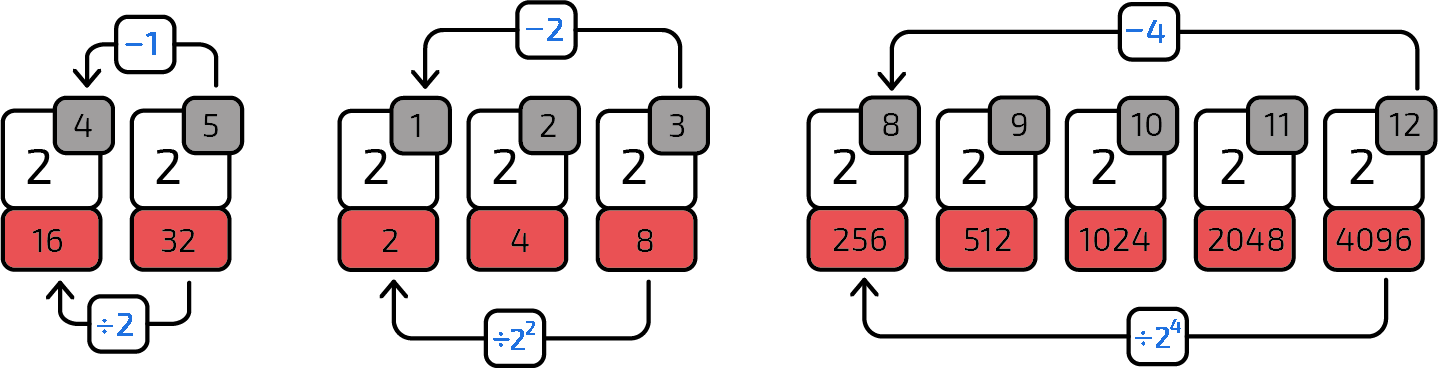
\includegraphics[width=\linewidth]{resp_inteiros_d.png}
\end{figure}


\end{enumerate}
}{1}
\end{answer}
\begin{answer}{Expoentes inteiros}
{
\begin{enumerate}\setcounter{enumi}{4}
\item
O esquema será:

\begin{figure}[H]
\centering
\noindent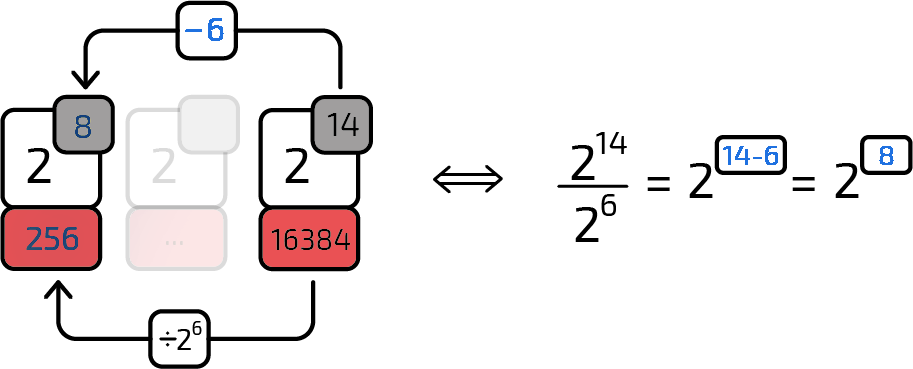
\includegraphics[width=.5\linewidth]{resp_inteiros_e.png}
\end{figure}

Alguns outros exemplos: $\dfrac{2^7}{2^5} =2^{7-5}=2^2$,\quad $\dfrac{2^{12}}{2^8} =2^{12-8}=2^4$. De um modo geral, se $m$ e $n$ são números inteiros então $\dfrac{2^m}{2^n} =2^{m-n}$.

\item Deverá ficar:

\begin{figure}[H]
\centering
\noindent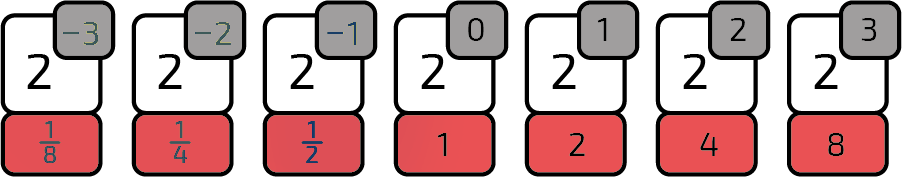
\includegraphics[width=.5\linewidth]{resp_inteiros_f.png}
\end{figure}

\item Teremos:

\begin{figure}[H]
\centering
\noindent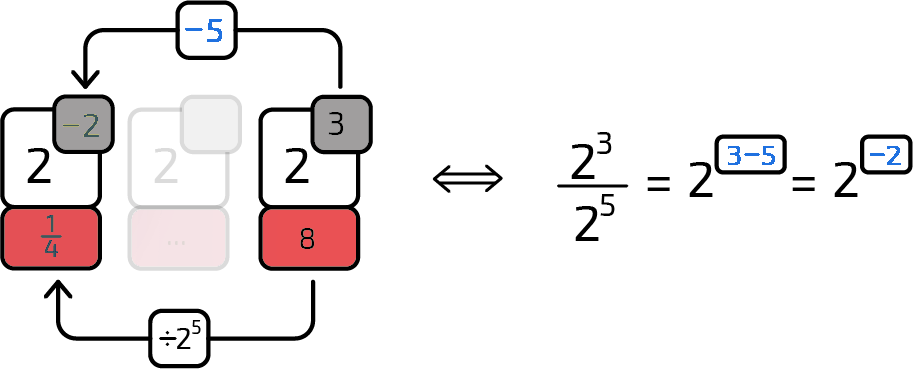
\includegraphics[width=.5\linewidth]{resp_inteiros_g.png}
\end{figure}

\item Completando o esquema vamos obter:

\begin{figure}[H]
\centering
\noindent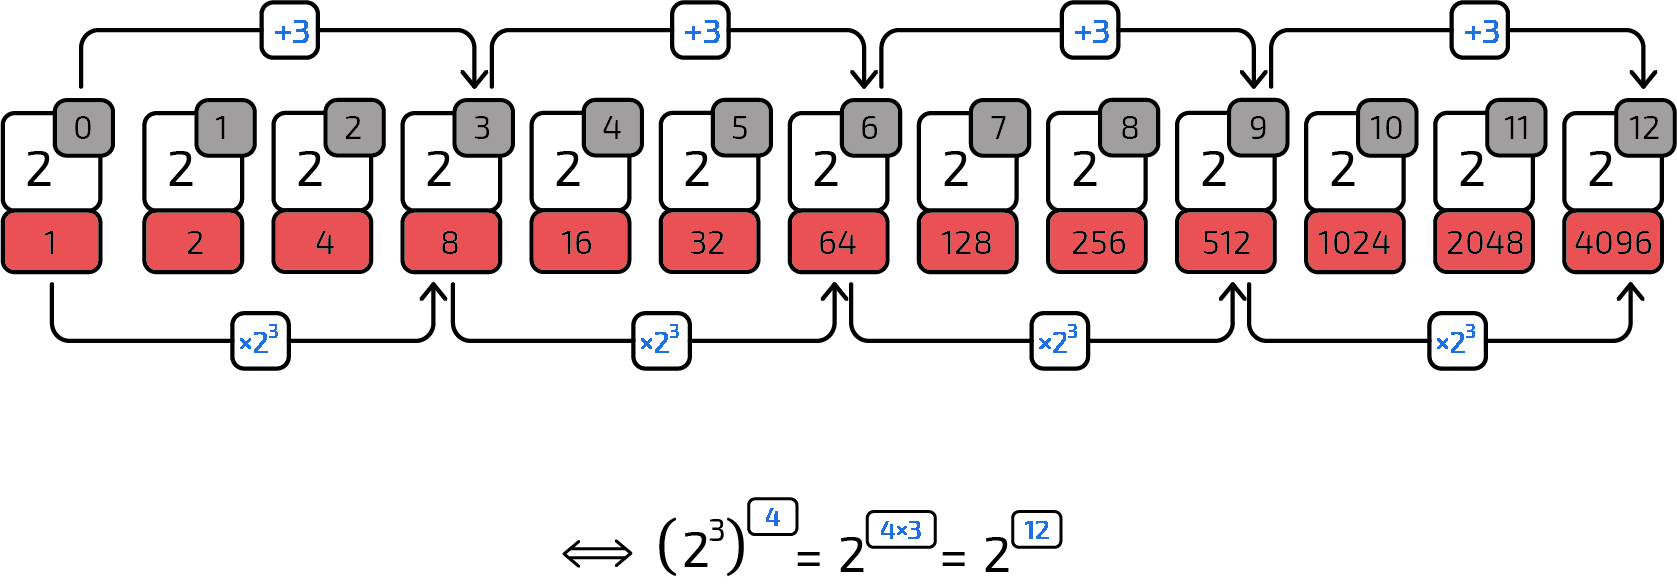
\includegraphics[width=.8\linewidth]{resp_inteiros_h.png}
\end{figure}

Alguns outros exemplos: $(2^{2})^{3}=2^{2\times3}=2^6$,\quad $(2^{8})^{5}=2^{8\times5}=2^{40}$. De um modo geral, se $m$ e $n$ são números inteiros então $(2^{m})^{n}=2^{m \times n}$.

\item (1)-(B),\quad (2)-(C),\quad (3)-(A).
\end{enumerate}
}{0}
\end{answer}
\clearmargin
\marginpar{\vspace{-1.5em}}
\begin{objectives}{Expoentes racionais}
{
\begin{itemize}
\item Revisar as propriedades aritméticas das potências com expoentes racionais;
\item Construir de modo intuitivo o significado de potências com expoentes inteiros racionais;

\end{itemize}
}{1}{1}
\end{objectives}
\marginpar{\vspace{-2.5em}}
\begin{sugestions}{Expoentes racionais}
{
\begin{itemize}

\item Esta atividade guarda bastantes semelhanças com a anterior, no sentido de que pode ser feita de maneira investigativa e que se trata de uma ampliação da definição de potência para expoentes racionais;

\item Alguns estudantes podem optar por representar os racionais na forma decimal e isto pode dificultar a percepção dos padrões. Sugira que estes também considerem trabalhar com frações;

\item Para muitos estudantes esse tema já deve ser conhecido do Ensino Fundamental, mas acreditamos que a maneira como expomos pode ajudar a construir uma intuição das justificativas/demonstrações das propriedades com expoentes racionais;

\item Essa intuição servirá de base para as discussões envolvendo a função exponencial de domínio real, onde abordaremos o cálculo do fator de crescimento, ou a imagem da função exponencial para tempos não inteiros.

\end{itemize}
}{1}{1}
\end{sugestions}
\begin{answer}{Expoentes racionais}
{
\begin{enumerate}

\item Completando os cartões obtemos:

\begin{figure}[H]
\centering
\noindent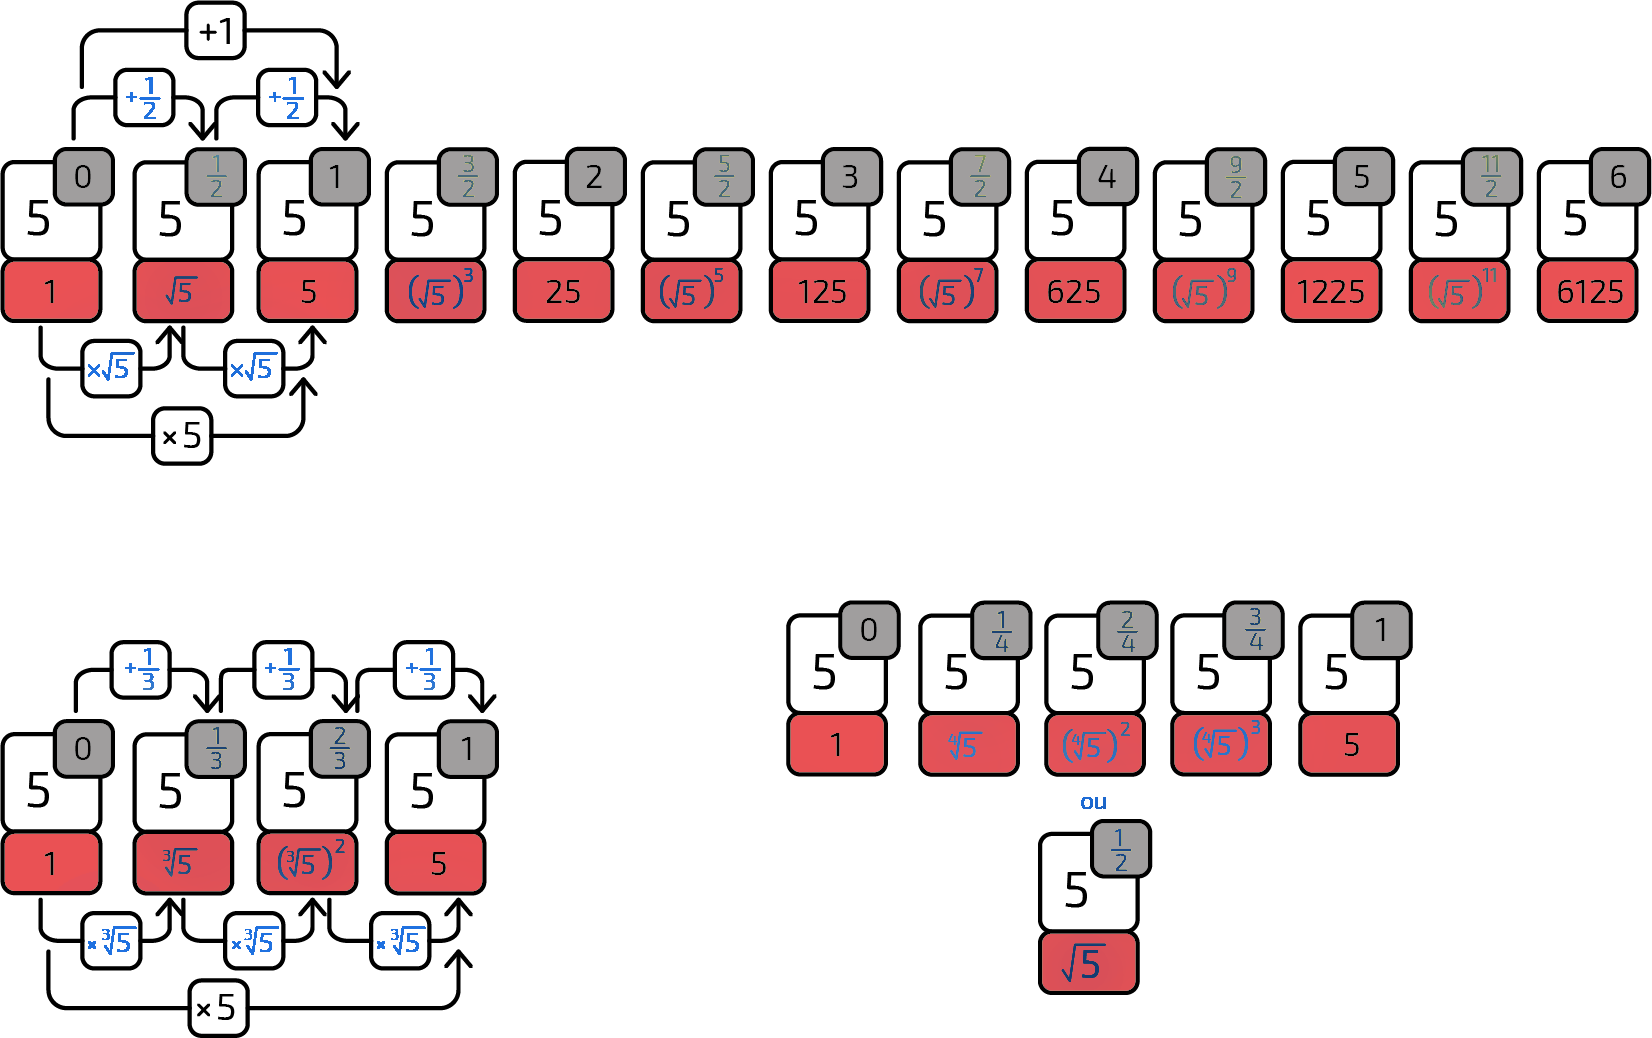
\includegraphics[width=.8\linewidth]{resp_racionais_a.png}
\end{figure}
\end{enumerate}
}{1}
\end{answer}
\begin{answer}{Expoentes racionais}
{
\begin{enumerate}
\item As expressões serão representadas por:

\begin{figure}[H]
\centering
\noindent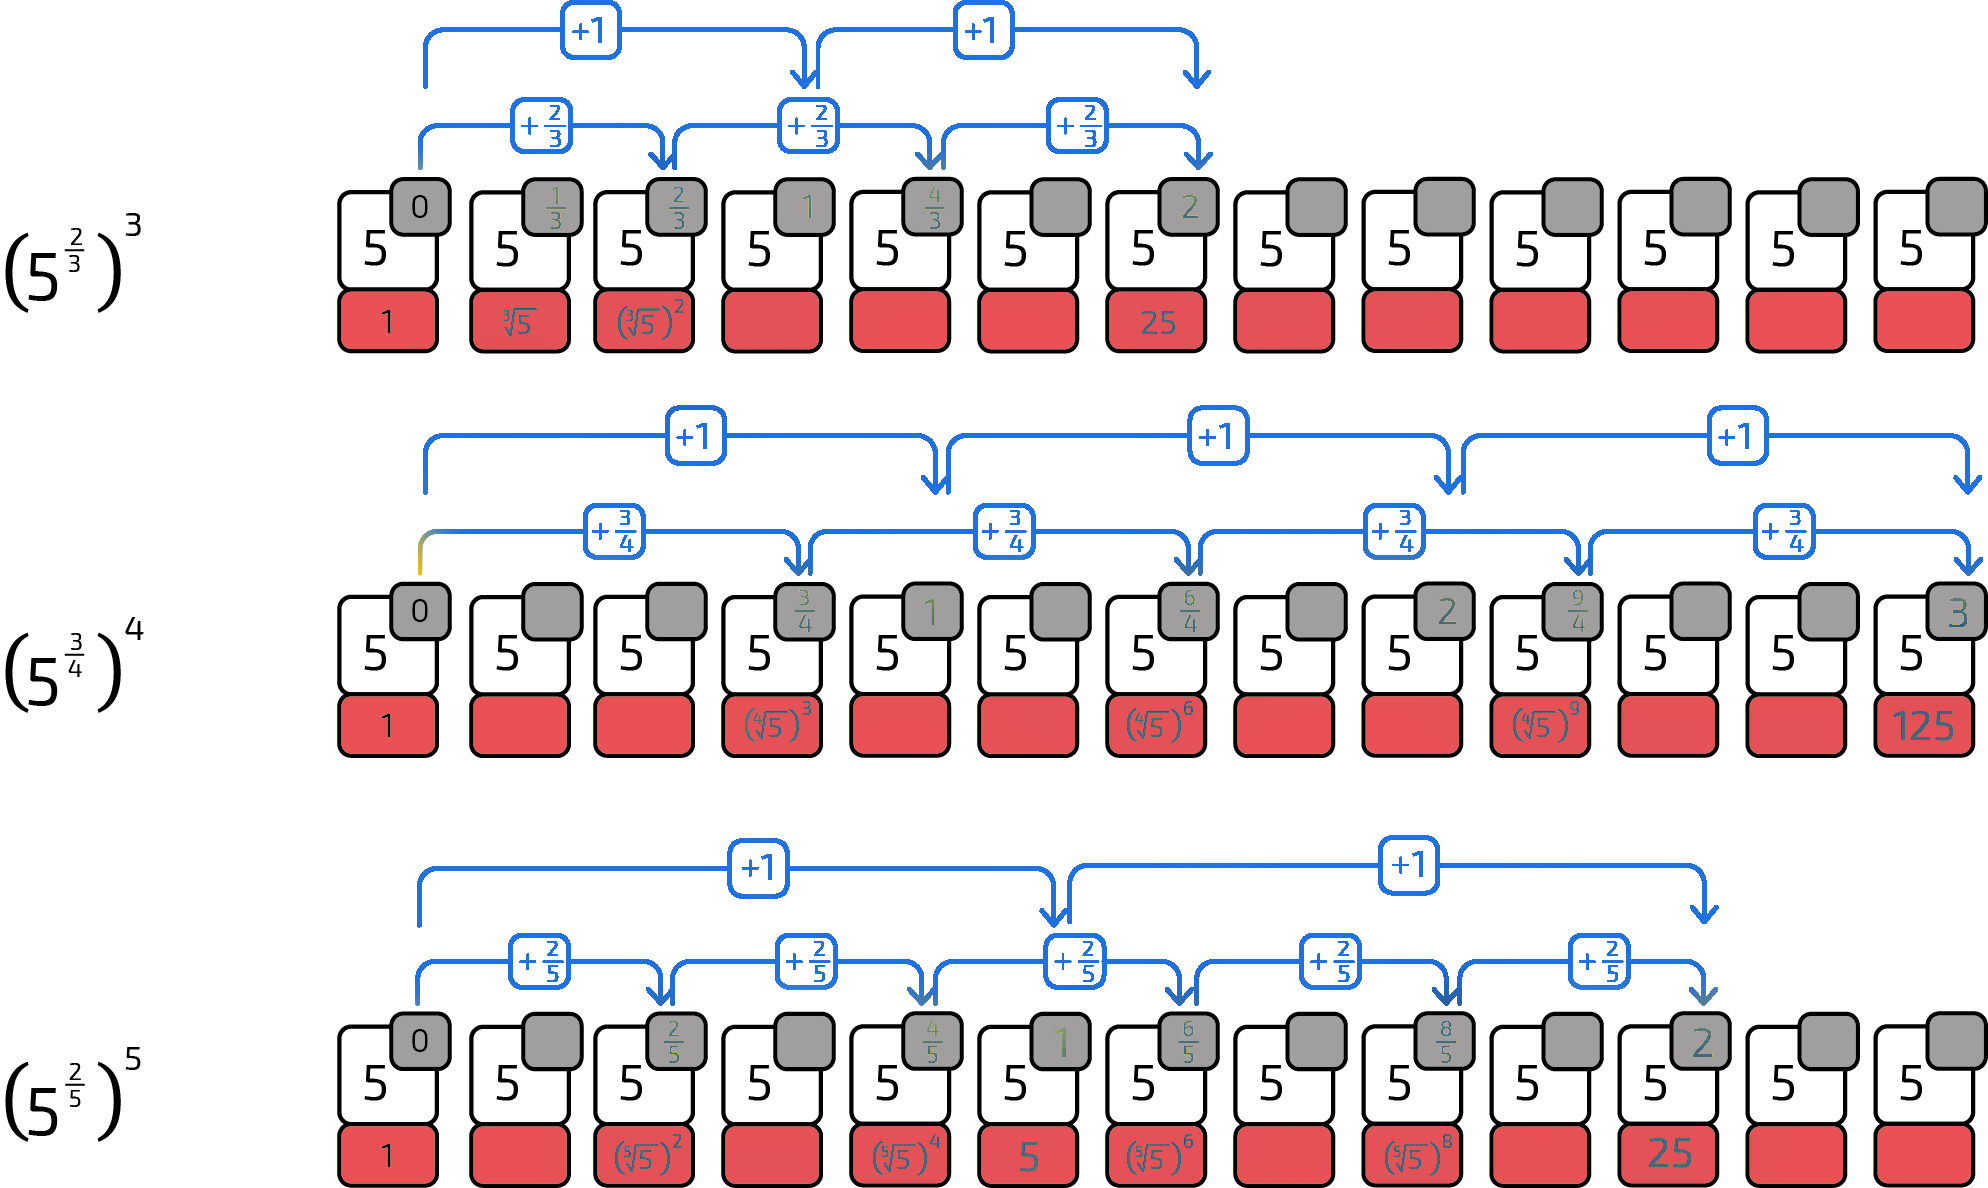
\includegraphics[width=\linewidth]{resp_racionais_b.png}
\end{figure}

\item $5^{\frac{m}{n}}=(\sqrt[n]{5})^{m}$.

\end{enumerate}
}{0}
\end{answer}

\explore{Propriedades Aritméticas}


\begin{task}{Expoentes inteiros}

Observe os cartões abaixo, e responda às perguntas que seguem.

\begin{figure}[H]
\centering
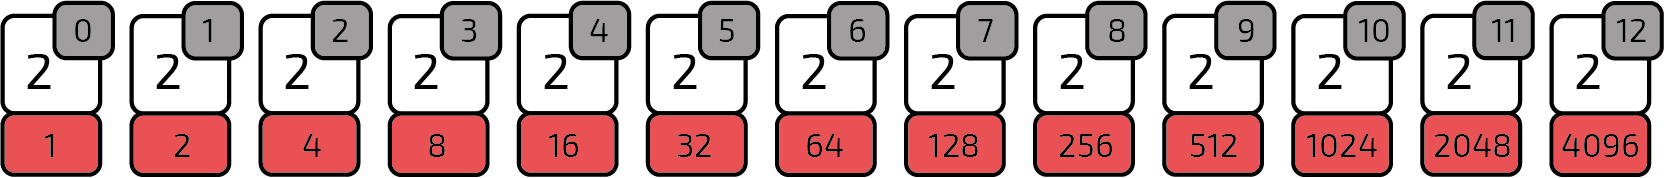
\includegraphics[width=.5\linewidth]{aritm1.png}
\end{figure}

\begin{enumerate}

\item{}
Que relação têm os números em um mesmo cartão?

\item{}
Que padrões se observam nos números em vermelho (embaixo) quando movemos para a \textbf{direita}? E nos números em cinza (acima)? Registre suas observações no esquema abaixo.

\begin{figure}[H]
\centering
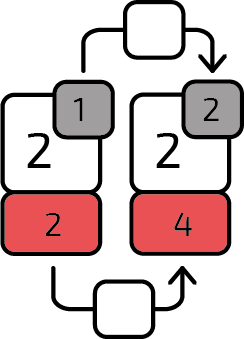
\includegraphics[width=65bp]{aritm2.png} \hspace{0,5cm}
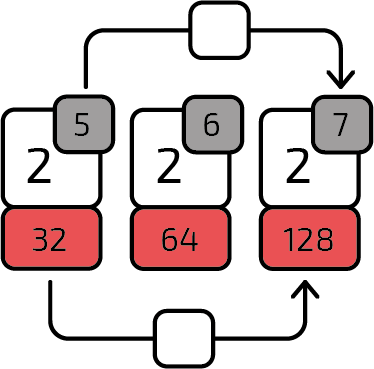
\includegraphics[width=90bp]{aritm3.png} \hspace{0,5cm}
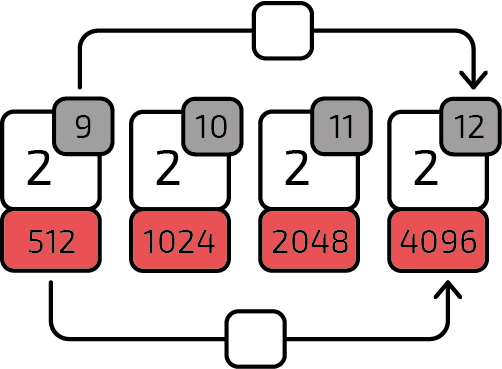
\includegraphics[width=120bp]{aritm4.png}
\end{figure}

\item{}
Complete o que falta no esquema abaixo. Escreva outros exemplos semelhantes e, então, generalize.

\begin{figure}[H]
\centering
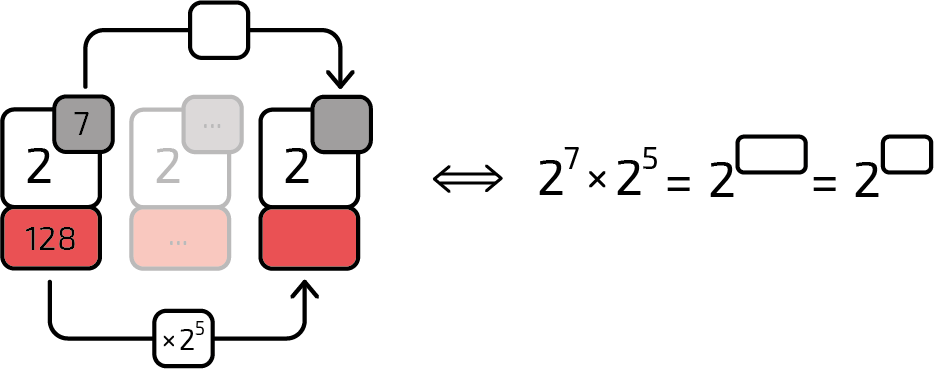
\includegraphics[width=200bp]{aritm5.png}
\end{figure}

\item{}
Que padrão se observa nos números em vermelho (embaixo) quando movemos para a \textbf{esquerda}? E nos números em cinza (acima)?

\begin{figure}[H]
\centering
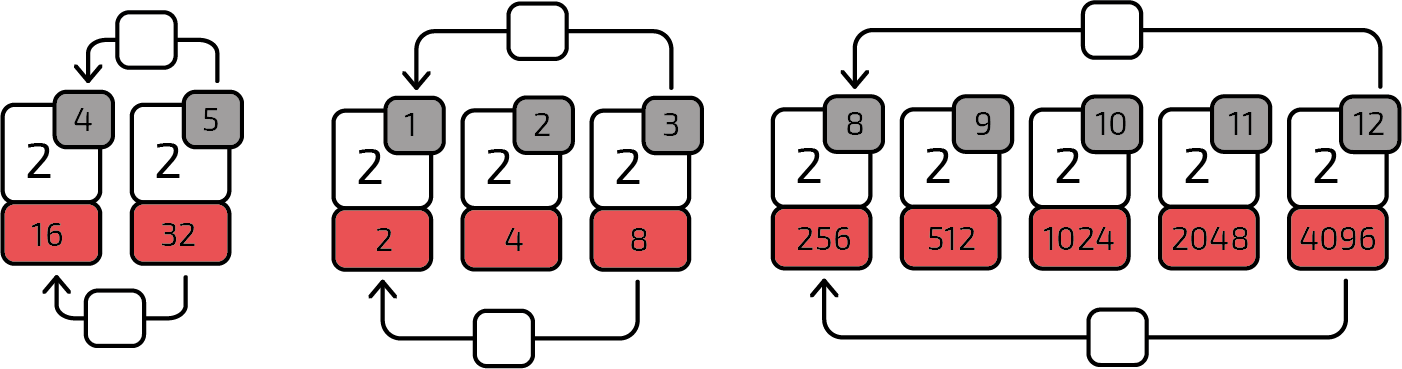
\includegraphics[width=280bp]{aritm6.png}
\end{figure}

\item{}
Complete o que falta no esquema abaixo. Escreva outros exemplos semelhantes e, então, generalize.

\begin{figure}[H]
\centering
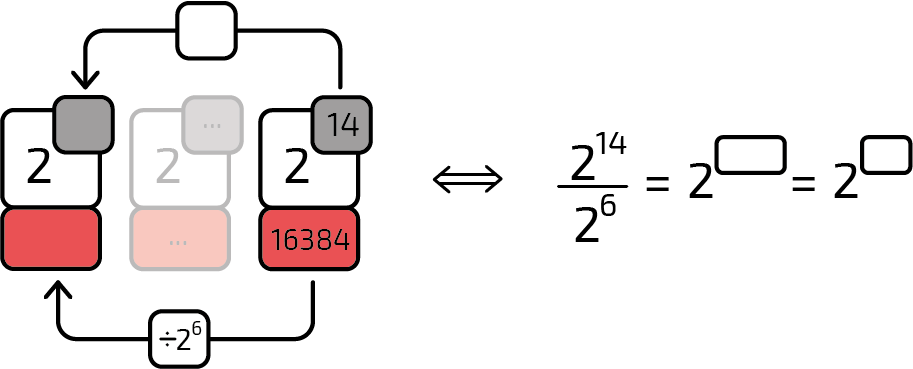
\includegraphics[width=220bp]{aritm7.png}
\end{figure}

\item{}
Proponha novos cartões, e explique suas escolhas.

\begin{figure}[H]
\centering
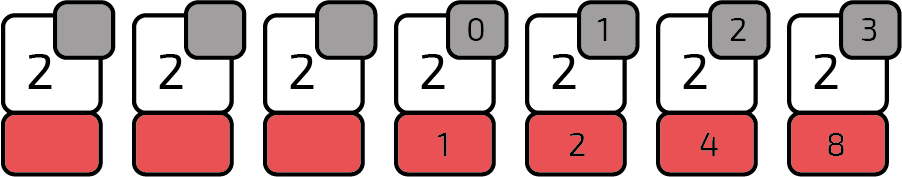
\includegraphics[width=200bp]{aritm8.png}
\end{figure}

\item{}
Baseado na sua proposta resolva.

\begin{figure}[H]
\centering
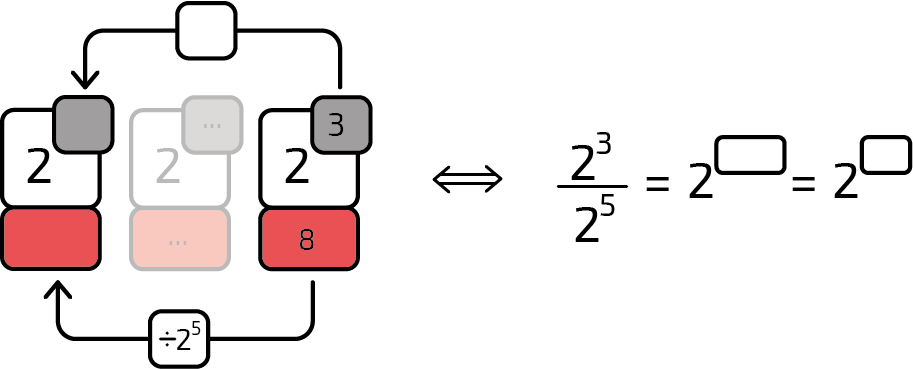
\includegraphics[width=200bp]{aritm9.png}
\end{figure}

\item{}
Complete o que falta no esquema abaixo. Escreva outros exemplos semelhantes e, então, generalize.

\begin{figure}[H]
\centering
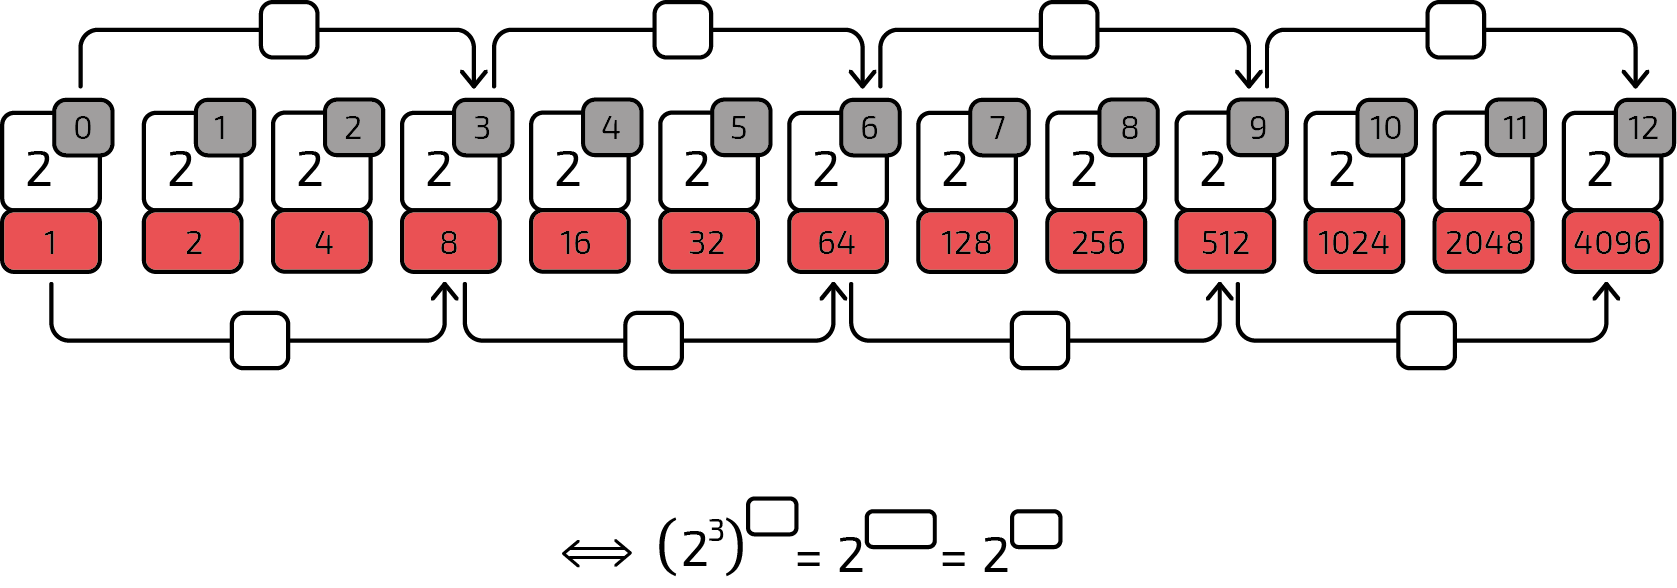
\includegraphics[width=300bp]{aritm10.png}
\end{figure}

\item{}
Sejam $m$ e $n$ números inteiros. Baseado nas suas conclusões nos itens anteriores, relacione a coluna da direita com a coluna da esquerda.

 (1) $2^{m} \cdot 2^{n}$  \hspace{1,0cm} (A) $2^{m \cdot n}$

 (2) $\dfrac{2^{m}}{2^{n}}$   \hspace{1,5cm} (B) $2^{m + n}$

 (3) $(2^{m})^{n}$  \hspace{1,1cm} (C) $2^{m - n}$

\end{enumerate}

\end{task}

\begin{task}{Expoentes racionais}

Observe os cartões e responda as perguntas.

\begin{enumerate}

\item{}
Completes os cartões vazios nas sequências abaixo. Explique seu raciocínio.

\begin{figure}[H]
\centering
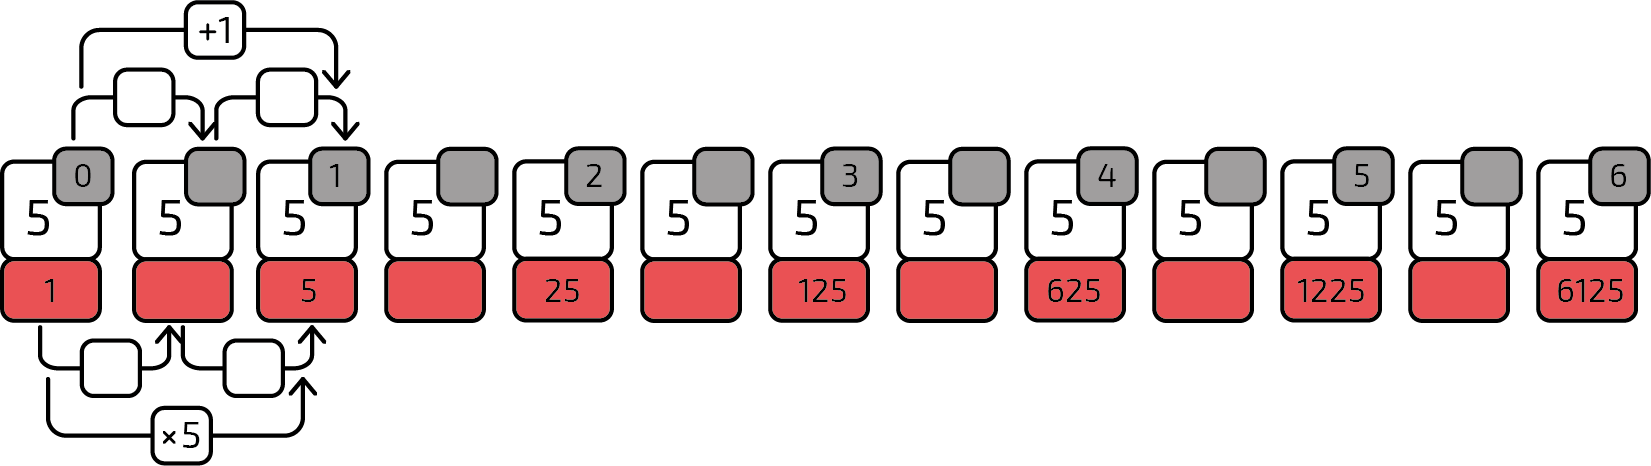
\includegraphics[width=300bp]{aritm11.png}
\end{figure}


\begin{figure}[H]
\centering
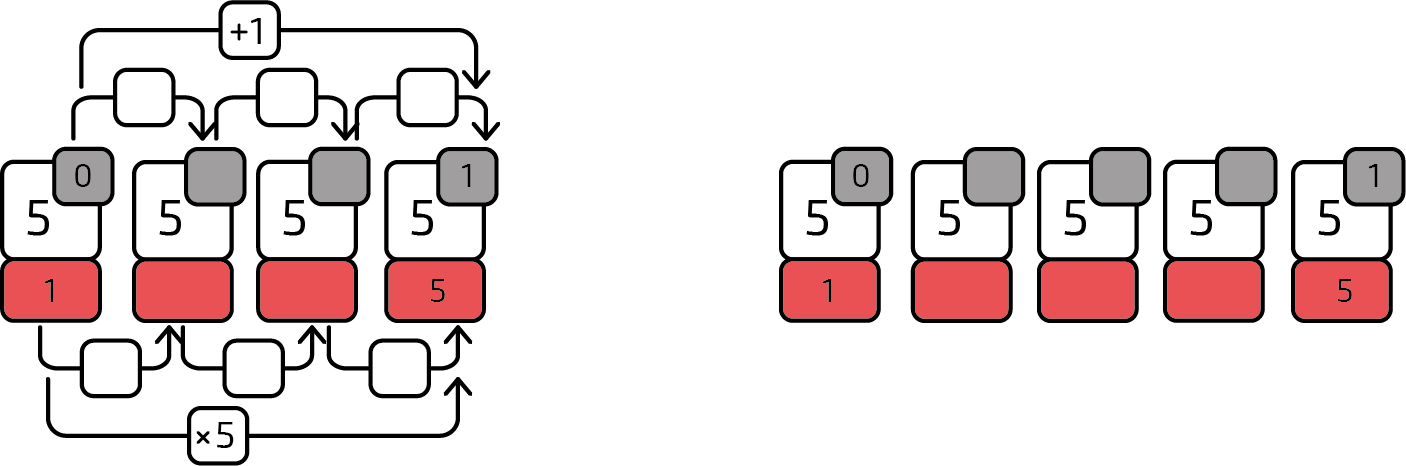
\includegraphics[width=300bp]{aritm12.png}
\end{figure}

\item{}
Represente nos cartões abaixo as expressões pedidas:

\begin{figure}[H]
\centering
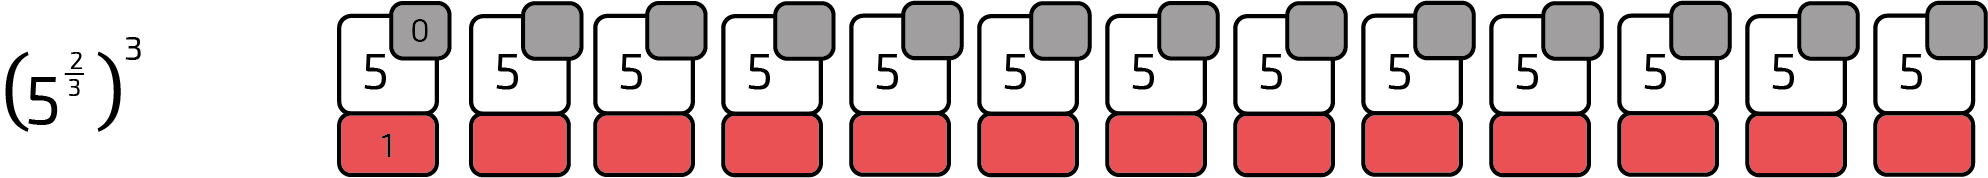
\includegraphics[width=350bp]{aritm13.png}
\end{figure}

\begin{figure}[H]
\centering
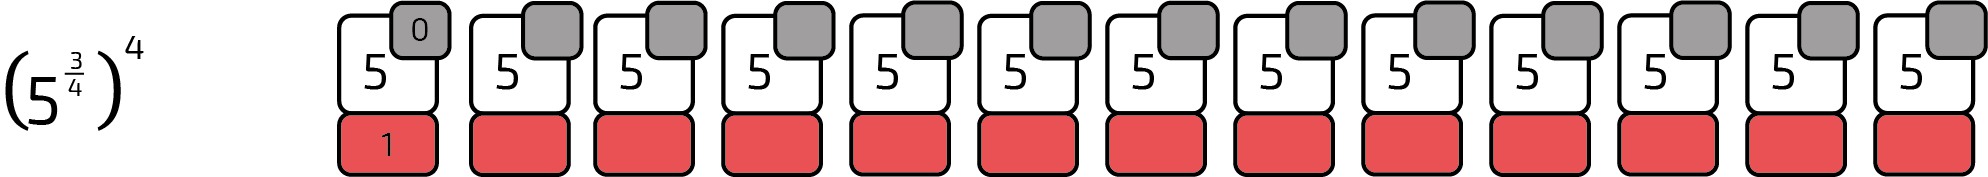
\includegraphics[width=350bp]{aritm14.png}
\end{figure}

\begin{figure}[H]
\centering
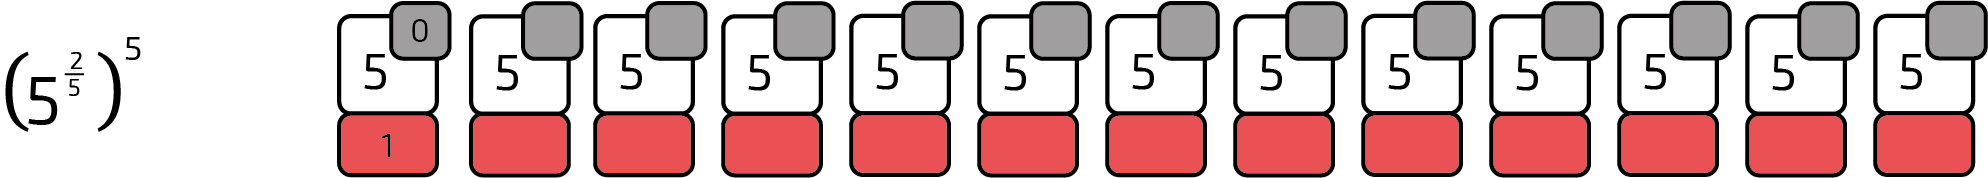
\includegraphics[width=350bp]{aritm15.png}
\end{figure}

\item{}
Qual a sua conclusão sobre que significado tem a expressão $5^{\frac{m}{n}}$ ?

\end{enumerate}

\end{task}

\begin{reflection}

Baseado nas propriedades discutidas nas duas atividades anteriores, que números reais estão representados pelas expressões?

 (a) $27^{-2/3}$  \hspace{1,5cm} (d) $3^{1/2}\cdot 3^{3/2}$ \hspace{1,5cm} (g) $\pi^{1/3} \cdot \pi^{1/2}$

 (b) $6^{-1/2}$   \hspace{1,7cm} (e) $3^{1/2+3/2}$  \hspace{1,7cm} (h) $(10^{1/2})^{1/3}$

 (c) $\left( \dfrac{1}{16}\right)^{-3/4}$  \hspace{1,0cm} (f) $\left( \dfrac{1}{2}\right)^{7/9} \cdot \left( \dfrac{1}{2}\right)^{2/9}$  \hspace{0,3cm} (i) $(10^{1/4})^{3/5}$

\end{reflection}

\arrange{Propriedades Aritméticas}

Como vimos nas investigações acima, quando realizamos operações matemáticas com números reais expressos na forma de potências podemos observar alguns padrões que se repetem quando relacionamos os resultados das potências e seus expoentes. De maneira resumida, podemos dizer que multiplicações e divisões entre potências correspondem a adições e subtrações entre seus expoentes. Vamos aqui, organizar essas propriedades.

Considere $m$ e $n$ dois números inteiros positivos, e $a$ um número real positivo, e diferente de $1$.

\begin{center}
\begin{tabular}{|c|c|}
\hline
$a^{m} \cdot a^{n} = a^{m+n}$                   &    \adjustbox{valign=c}
{
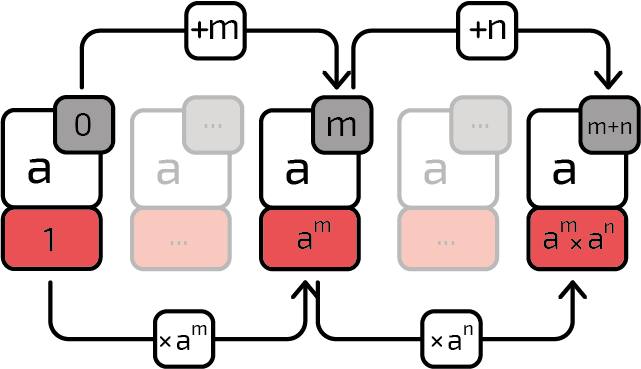
\includegraphics[scale=0.7]{aritm16.png}
}          \\ \hline
$ (a^{m})^{n} = a^{m \cdot n}$                    &    \adjustbox{valign=c}
{
\includegraphics[scale=0.7]{aritm17.png}
}            \\ \hline
$ \dfrac{1}{a^{m}} = a^{-m}$                    &    \adjustbox{valign=c}
{
\includegraphics[scale=0.7]{aritm18.png}
}            \\ \hline
$ \dfrac{a^{m}}{a^{n}} = a^{m - n}$                    &    \adjustbox{valign=c}
{
\includegraphics[scale=0.7]{aritm19.png}
}            \\ \hline
$ \left( a^{m/n}\right)^{n} = a^{m} \iff a^{m/n} = \sqrt[n]{a^{m}}$                     &    \adjustbox{valign=c}
{
\includegraphics[scale=0.7]{aritm20.png}
}            \\ \hline
\end{tabular}
\end{center}

Até agora sabemos calcular e operar potências com expoentes inteiros (positivos, zero e negativos) e também racionais. Vamos ver como esses números aparecem nas representações gráficas. Neste link \url{https://www.geogebra.org/m/xatdbug7} você pode acessar uma versão interativa dos gráficos mostrados a seguir, em que consideramos separadamente os casos $0<a<1$ e $a>1$.

Vamos considerar uma função exponencial do tipo $y=a^{x}$ com $a>1$. O caso $0<a<1$ é inteiramente análogo.

Estendendo para valores inteiros negativos de $x$, teremos algo como no gráfico abaixo. Uma base $a>1$ elevada a um expoente negativo é sempre um número positivo e menor que $1$.
\[
a>1 \iff 0<a^{-n}<1
\]

\begin{figure}[H]
\centering
\includegraphics[width=300bp]{rac1.png}
\end{figure}

Perceba no gráfico, que os pontos do lado esquerdo do eixo $y$ estão todos acima do gráfico (positivos) e abaixo do ponto que está sobre o eixo (menores que $1$). Observe também que quanto mais negativo é o expoente, mais próximo de zero estará o resultado da potência. O gráfico mantém o aspecto crescente: para $m$ e $n$ inteiros, temos

\[
m>n \Rightarrow a^{m}>a^{n}
\]

Se acrescentamos agora as frações de denominador 2, ou seja os pontos médios entre os valores de x inteiros, teremos o seguinte aspecto.

\begin{figure}[H]
\centering
\includegraphics[width=300bp]{rac2.png}
\end{figure}

As propriedades gráficas anteriores todas se mantêm: gráfico crescente (com crescimento rápido para valores de x positivos), sempre acima do eixo x, se aproximando de zero à medida que o valores do domínio são números negativos cada vez menores.

Acrescentando outras frações, os pontos vão se acumulando mantendo sempre o mesmo aspecto visual.

\begin{figure}[H]
\centering
\includegraphics[width=300bp]{rac3.png}
\end{figure}

O último gráfico parece ser uma linha contínua, mas é apenas uma questão de escala: basta aproximar para um intervalo menor e ver que os pontos estão, na verdade, espaçados. O processo continua indefinidamente. Podemos aumentar o denominador nessa janela até parecer novamente contínuo e depois aproximar até ver os espaços entre os pontos.

\begin{figure}[H]
\centering
\includegraphics[width=300bp]{rac4.png}
\end{figure}

\begin{figure}[H]
\centering
\includegraphics[width=300bp]{rac5.png}
\end{figure}

\begin{figure}[H]
\centering
\includegraphics[width=300bp]{rac6.png}
\end{figure}

Por se tratar de um processo infinito, podemos repeti-lo tantas vezes quanto desejamos de forma que será possível, definir também as potências com expoentes irracionais.

Como se sabe, os números irracionais não podem ser escritos na forma de fração, mas podem ser bem aproximados por números racionais.

Vejamos o caso do número $2^{\sqrt{2}}$. (versão interativa \url{https://www.geogebra.org/m/zdyqhhwb} )

\begin{figure}[H]
\centering
\includegraphics[width=300bp]{irrac1.png}
\end{figure}

\begin{figure}[H]
\centering
\includegraphics[width=300bp]{irrac2.png}
\end{figure}

\begin{figure}[H]
\centering
\includegraphics[width=300bp]{irrac3.png}
\end{figure}

\begin{figure}[H]
\centering
\includegraphics[width=300bp]{irrac4.png}
\end{figure}

\begin{figure}[H]
\centering
\includegraphics[width=300bp]{irrac5.png}
\end{figure}

\begin{eqnarray*}
{\sqrt{2}}&\approx& 1,414213562...\\
2^{1{,}4}\approx 2{,}6390158215...& <2^{\sqrt{2}} < & 2^{1{,}5}\approx 2{,}8284271247...\\
2^{1{,}41}\approx {\color{red} 2{,}6}573716281... & < 2^{\sqrt{2}} < & 2^{1{,}42}\approx {\color{red} 2{,}6}758551095...\\
2^{1{,}414}\approx {\color{red} 2{,}66}47496501...&<2^{\sqrt{2}} < & 2^{1{,}415}\approx {\color{red} 2{,}66}65973541...\\
2^{1{,}4142}\approx {\color{red} 2{,}665}1190885...&<2^{\sqrt{2}} <& 2^{1{,}4143}\approx {\color{red} 2{,}665}3038269...\\
2^{1{,}41421}\approx {\color{red} 2{,}6651}375617...&<2^{\sqrt{2}} <& 2^{1{,}41422}\approx {\color{red} 2{,}6651}560351...\\
2^{1{,}414213}\approx {\color{red} 2{,}66514}3103...&<2^{\sqrt{2}} <& 2^{1{,}414214}\approx {\color{red} 2{,}66514}49511...\\
2^{1{,}4142135}\approx {\color{red} 2{,}665144}0274...&<2^{\sqrt{2}} <& 2^{1{,}4142136}\approx {\color{red} 2{,}665144}212...\\
2^{1{,}41421356}\approx {\color{red} 2{,}6651441}383... &<2^{\sqrt{2}} <& 2^{1{,}41421357}\approx {\color{red} 2{,}6651441}567... \\
2^{1{,}414213562}\approx {\color{red} 2,66514414}2.. &<2^{\sqrt{2}} <& 2^{1{,}414213563}\approx {\color{red} 2{,}66514414}38...\\
&\therefore& \\
2^{\sqrt{2}}&\approx& 2{,}66514414...\\
\end{eqnarray*}

O valor que obtemos com esse processo (mesmo que façamos muitas etapas) é uma aproximação racional do número $2^{\sqrt{2}}$, que é um número irracional. Mas, o grande interesse aqui não é no valor numérico de uma potência com expoente irracional, porque isso pode ser feito em qualquer calculadora científica ou mesmo nos principais sites de busca, por exemplo, para $2^{\sqrt{2}}$ basta digitar $ \boxed{2}$\ ,  $\boxed{x^y}$ ou $\boxed{\land}$\ ,  $\boxed{\sqrt{\ }}$ ou  $\boxed{sqrt}$ e $\boxed{2}$\ , mas entender que tais números podem ser definidos a partir de um processo de aproximação por potências cujos expoentes são racionais (frações), e que, além disso podem ser operados obedecendo às mesmas propriedades que valem para os expoentes racionais.

\begin{figure}[H]
\centering
\includegraphics[width=3cm]{calc.png}
\includegraphics[width=5cm]{calc2.png}
\caption{Calculadora Android e página de busca do Google.}
\end{figure}

Na próxima seção faremos uma revisão sobre tais propriedades quando definirmos a função exponencial com domínio real.

\begin{knowledge}
Experimente digitar em uma calculadora convencional o número $\boxed{2}$ seguido da tecla $\boxed{\sqrt{\ }}$ (ou na ordem contrária na calculadora do celular, isto é, aperte $\boxed{\sqrt{\ }}$ seguido de $\boxed{2}$. 

Observe o número aparece no visor da calculadora. Será correto afirmar que $\sqrt{2}$ é \textbf{igual} a este resultado, isto é, que $\sqrt{2}=1{,}414213562$ ? Experimente agora digitar esse número $1{,}414213562$ e elevá-lo ao quadrado. O resultado que aparece é $2$?

Embora apertemos a tecla $\boxed{=}$, o resultado dado pela calculadore, neste caso, é apenas aproximado, e isso ocorre porque as calculadoras (e os computadores) são máquinas capazes de armazenar e manipular apenas quantidades finitas de dados. Por isso, quando elas tem que armazenar ou fazer contas com números que não admitem uma representação decimal finita, como é o caso dos números irracionais, o que elas fazem é trabalhar com aproximações destes números. A boa notícia é que para a grande maioria das situações isso é bom o suficiente. 

Existem duas subáreas da Matemática que lidam com aproximações deste tipo: uma mais teórica chamada de \textit{Teoria dos Números} que tem uma parte de seus resultados dedicados a classificar aproximações de números irracionais, e outra mais aplicada chamada \textit{Análise Numérica} que se ocupa, dentre outras coisas, do estudo das propagações de erros em algoritmos feitos por computadores para resolver problemas matemáticos.

\end{knowledge}

\cleardoublepage
\def\currentcolor{session1}
\begin{objectives}{Um cafézinho}
{
\begin{itemize}
\item Compreender o significado de potências com expoentes racionais nas situações problema.

\end{itemize}
}{1}{1}
\end{objectives}
\begin{sugestions}{Um cafézinho}
{
\begin{itemize}
\item Oferecemos nesta atividade um exemplo com dados reais em que aparecem expoentes não inteiros. Havendo disponibilidade você pode ou mostrar para a turma a animação desta situação disponível neste link \url{https://www.desmos.com/calculator/nn0f7iw3tz} ou indicar que eles assistam.

\item Destaque que a quantidade inicial de cafeína no organismo do indivíduo de que trata a questão é obtida tomando t=0 na função.

\item Em processos envolvendo decaimento exponencial é interessante identificar o intervalo de tempo necessário para que a quantidade inicial decaia pela metade. Você pode utilizar a animação em GeoGebra disponível neste endereço \url{https://www.geogebra.org/m/qgfuymx9} para ilustrar graficamente esse processo.

\end{itemize}
}{1}{1}
\end{sugestions}
\begin{answer}{Um cafézinho}
{
\begin{enumerate}
\item
As quantidades de cafeína no organismo do indivíduo meia hora (0,5), uma hora e meia (1,5) e quatro horas (4) após a ingestão da xícara de café serão, respectivamente, dadas por:

$f(0,5)=94{,}39$mg, \quad $f(1,5)=84{,}09$mg, \quad $f(4)=63$mg.

\item $50=100\cdot(0,5)^{\frac{t}{6}}\iff\dfrac{1}{2}=\left( \dfrac{1}{2} \right)^{\frac{t}{6}}$ $\iff$ $t=6$ horas.

\item $F(t)=150\cdot(0{,}5)^{\frac{t}{8}}$.

\end{enumerate}
}{1}
\end{answer}
\clearmargin
\begin{objectives}{Qual é a expressão?}
{
\begin{itemize}
\item Deduzir expressões de funções exponenciais envolvendo expoentes racionais, a partir de situações problema.

\end{itemize}
}{1}{2}
\end{objectives}
\begin{sugestions}{Qual é a expressão?}
{
\begin{itemize}
\item A ideia central é que se a cada $4$ dias o número de infectados triplica, a cada dois dias ficará multiplicado por $\sqrt{3}$, e cada $1$ dia ficará multiplicado por $\sqrt[4]{3}=\sqrt{\sqrt{3}}$. E isso levará à expressão $3^{\frac 14}$.

\item Como estamos propondo uma simulação de dados reais, é possível trabalhar com uma margem de aproximações para os valores colocados.

\item Ao término da atividade, durante as discussões, proponha algumas generalizações como: qual seria a fórmula se houvesse $200$ infectados no início? Se quintuplicasse a cada $4$ dias? Se quadruplicasse a cada $5$ dias? etc.

\end{itemize}
}{1}{2}
\end{sugestions}
\begin{answer}{Qual é a expressão?}
{
\begin{enumerate}

\item $300, 900, 2700, 8100, 24300$

\item $100\sqrt{3} \approx 173$ e $300\sqrt{3} \approx 519$

\item $131, 173, 227, 300, 395, 520, 684, 900$. Para obter o valor do dia seguinte, multiplicar o anterior por $\sqrt[4]{3}$.

\item Modelo (III).
\end{enumerate}
}{1}
\end{answer}
\clearmargin
\begin{objectives}{Afim e Exponencial}
{
\begin{itemize}
\item Investigar por meio de gráficos as variações da função exponencial em intervalos de tamanho fixo, comparando com a variações da função afim.

\item Identificar os papéis das constantes na expressão da função exponencial $f(x)=ca^{\frac xk}$.

\end{itemize}
}{1}{1}
\end{objectives}
\begin{sugestions}{Afim e Exponencial}
{
\begin{itemize}
\item Após a discussão peça para os estudantes proporem desafios para os colegas: eles mostram $3$ pontos e os colegas tentam “adivinhar” o próximo e fornecer a expressão analítica.

\end{itemize}
}{1}{1}
\end{sugestions}
\begin{answer}{Afim e Exponencial}
{
\begin{enumerate}

\item $3$ é o intercepto-y, $1$ é o deslocamento vertical que corresponde a um deslocamento horizontal de $4$ unidades.

\item
$1$ é o intercepto-y (valor inicial), a cada $4$ unidades de deslocamento horizontal o valor anterior fica multiplicado por $3$.

\item
Valor inicial $4$ e a cada $5$ unidades de deslocamento horizontal, multiplicamos por $\frac 64=\frac 32$. Assim, para $x=15$ teremos $f(15)=9\cdot \frac 32=13{,}5$.
A expressão então é dada por $f(x)=4\cdot \left(\dfrac 32\right)^{\frac x5}$.

\end{enumerate}
}{1}
\end{answer}


\explore{Função exponencial}

\begin{task}{Um cafézinho}

Chamamos meia-vida biológica da cafeína o tempo necessário para que o nosso corpo elimine a metade de uma dose desta substância. Esse tempo varia amplamente entre os indivíduos de acordo com fatores como gravidez, ingestão outras drogas, nível de função enzimática hepática (necessário para o metabolismo da cafeína) e idade. Em adultos saudáveis, a meia-vida da cafeína varia entre três a sete horas. Nos recém-nascidos, a meia-vida da cafeína pode ser de $80$ horas ou mais, sendo esta uma das razões para a recomendação  de não dar qualquer alimento que contenha cafeína para bebês.
Fonte: \url{https://pt.wikipedia.org/wiki/Cafe\%C3\%ADna}

\begin{figure}[H]
\centering
\includegraphics[width=250bp]{cafeina.png}
\caption{Gráfico mostrando como a quantidade de cafeína no organismo de um indivíduo que ingeriu uma xícara de café de $250 ml$ varia ao longo do tempo (medido em horas).}
\end{figure}

Para um indivíduo que acabou de ingerir uma xícara de café de $250 ml$ - que contém cerca de $100 mg$ de cafeína - exames laboratoriais mostraram que a quantidade de cafeína no seu organismo variou com o passar do tempo (em horas) de acordo com a seguinte função $f(t)=100 \cdot (0{,}5)^{\frac{t}{6}}$, pergunta-se:

\begin{enumerate}

\item{}
Quais serão as quantidades de cafeína no organismo deste indivíduo após meia hora, uma hora e meia e quatro horas desde a ingestão da xícara de café ?

\item{}
Quanto tempo deverá se passar desde a ingestão da xícara de café até que a quantidade de cafeína no organismo deste indivíduo caia para a metade da quantidade inicial ?

\item{}
Que mudanças deveríamos fazer na expressão caso a meia-vida da cafeína neste indivíduo fosse de $8$ horas e ele tivesse ingerido 150 mg de cafeína?

\end{enumerate}

\end{task}

\begin{task}{Qual é a expressão?}

Uma epidemia causada por um vírus está se espalhando na cidade. Os cientistas, após analisarem os primeiros dados concluem que a doença está se espalhando rapidamente porque o número de infectados está triplicando a cada $4$ dias. O número inicial de infectados que compuseram a análise foi de $100$ pessoas. Responda as perguntas.

\begin{enumerate}

\item{} Complete a tabela com os possíveis números de infectados observados pelos cientistas.

%\begin{figure}[H]
%\centering
%\includegraphics[width=300bp]{infectados.png}
%\end{figure}
\begin{center}
	\begin{tabular}{|c|c|c|c|c|c|c|}
		\hline
		\tcolor{Infectados}                                                                             & \tcolor{100} & \tcolor{}  & \tcolor{}  &  \tcolor{}  &  \tcolor{}  &  \tcolor{}  \\ \hline
		\begin{tabular}[c]{@{}c@{}}Dias desde o \\ $100^\circ$ caso \\ confirmado\end{tabular} & 0   & 4 & 8 & 12 & 16 & 20 \\ \hline
	\end{tabular}
\end{center}

\item{} Considerando que esse modelo retrata bem a realidade, ou seja, que a evolução do número de casos obedece a um padrão de crescimento exponencial, qual deve ser o número aproximado de infectados no segundo e no sexto dias desde o $100^\circ$ confirmado?

\begin{center}
	\begin{tabular}{|c|c|c|c|c|c|}
\hline
\tcolor{Infectados}                                                                    & \tcolor{100} & \tcolor{}  & \tcolor{}  & \tcolor{} \tcolor{} &  \tcolor{} \\ \hline
\begin{tabular}[c]{@{}c@{}}Dias desde o\\ $100^{\circ}$ caso\\ confirmado\end{tabular} & 0   & 2 & 4 & 6 & 8 \\ \hline
\end{tabular}
\end{center}

\item{} Complete a tabela abaixo,  com a possível evolução diária dos casos. Explique seu raciocínio.

\begin{center}
	\begin{tabular}{|c|c|c|c|c|c|l|l|l|l|}
\hline
\tcolor{Infectados}                                                                    & \tcolor{100} &  \tcolor{} & \tcolor{}  &  \tcolor{} & \tcolor{}  &  \tcolor{} & \tcolor{}  & \tcolor{}  &  \tcolor{} \\ \hline
\begin{tabular}[c]{@{}c@{}}Dias desde o\\ $100^{\circ}$ caso\\ confirmado\end{tabular} & 0   & 1 & 2 & 3 & 4 & 5 & 6 & 7 & 8 \\ \hline
\end{tabular}
\end{center}

\item{} Denotando por $D(t)$ o número de infectados $t$ dias após o $100º$ caso confirmado, qual dos modelos exponenciais abaixo melhor representa $D(t)$.

(I) $D(t)=100 \cdot 3^{t+4}$

(II) $D(t)=100 \cdot 3^{4t}$

(III) $D(t)=100 \cdot 3^{\frac t4}$

\end{enumerate}

\end{task}


\begin{task}{Afim e Exponencial}


\begin{figure}[H]
\centering
\includegraphics[width=5cm]{grafico_afim.png}
\includegraphics[width=5cm]{grafico_exp.png}
\end{figure}

\begin{enumerate}

\item{} O gráfico (A) representa a função afim $y=3+\dfrac{1}{4}x$. Explique como os números $3$, $1$ e $4$ que aparecem na expressão da função afetam ou “aparecem” no gráfico.

\item{} O gráfico (B) representa o crescimento exponencial dado pela expressão $y=1 \cdot 3^{x/4}$. Explique como os números $3$, $1$ e $4$ que aparecem na expressão da função afetam ou “aparecem” no gráfico.

\item{} Os três pontos representados abaixo pertencem a uma curva de crescimento exponencial. Determine o ponto de abscissa $x=15$ que mantém esse crescimento e escreva uma expressão que descreva a curva.

\begin{figure}[H]
\centering
\includegraphics[width=170bp]{pontos.png}
\end{figure}

\end{enumerate}

\end{task}


\arrange{Função Exponencial}

Até aqui aprendemos a identificar e quantificar o crescimento (ou decaimento) exponencial, inclusive em termos percentuais. Vimos também que a expressão $f(x) = c \cdot a^{x}$ é a que descreve situações em que há crescimento/decaimento exponencial. Daremos agora o passo seguinte, isto é, vamos olhar para a expressão $f(x) = c \cdot a^{x}$ como uma função de variável real, ou seja, cujo domínio é todo o conjunto dos números reais. Você pode então se perguntar, mas o que muda em relação ao que vínhamos fazendo até aqui? Em termos práticos, agora podemos calcular a imagem de qualquer número real que faça sentido no contexto do problema sem termos que nos preocupar se ele é ou não múltiplo inteiro do período em que se multiplica o fator de crescimento/decaimento. No que diz respeito aos gráficos, podemos desenhar linhas contínuas com comportamentos bem definidos (e não mais marcar pontos a partir dos dados de uma tabela).

\begin{description}
\item[Definição] Chama-se função exponencial a função de domínio real $f: \mathbb{R} \rightarrow \mathbb{R}$ que pode ser escrita da forma $f(x)= c \cdot a^{x}$ em que $a$ é um número real positivo e diferente de $1$ e $c$ é um número positivo.
\end{description}

\begin{reflection}

Por que você acha que precisamos  fazer as restrições nos valores da base? O que acontece se $a=0$, $a=1$, ou se $a$ é negativo?

\begin{figure}[H]
\centering
\includegraphics[width=275bp]{exp.png}
\end{figure}

Se a base $a$ é um número positivo menor que $1$, estamos diante de uma função exponencial decrescente. Caso $a$ seja maior que $1$, teremos uma função crescente. Os gráficos, em ambos os casos, ficam acima do eixo $x$, isto é, à região correspondente às ordenadas positivas, e intersectam o eixo das ordenadas no ponto $(c,0)$.

O \textbf{conjunto imagem} da função exponencial $f(x) = c \cdot a^{x}$ é o conjunto de todos números reais positivos. Para se convencer desse fato, pense por exemplo na função $y = 10^x$: qualquer número real $y_0$ positivo, (muito) grande ou (muito) pequeno, está entre duas potências consecutivas de 10 (podendo ser uma delas). Ou seja, existe um número inteiro $k$ tal que
\[
10^k\leqslant y_0 <10^{k+1}
\]
Uma vez localizado esse intervalo $ [k,k+1[ $, podemos considerar os (infinitos) números racionais e irracionais nele para ir aproximando até localizar o valor $x_0$ tal que $10^x_0=y_0$. 

A mesma coisa vale para qualquer outra base a > 0 e diferente de 1. (esses fatos serão explorados um pouco mais no capítulo de função logarítmica: esse expoente $x_0$ que encontramos se chama o logaritmo de $y_0$ na base 10).

Você pode explorar mais e aprender sobre os aspectos visuais do gráfico da função exponencial neste link \url{https://www.geogebra.org/m/qvphqptp}.

\end{reflection}

\begin{observation}{Observações}

 \textbf{1.} As propriedades aritméticas que vimos anteriormente e que valem para quaisquer números reais $x$, $x'$ são

\begin{itemize}

\item{} $a^{x+x'} = a^{x}  \cdot a^{x'}$

\item{} $a^{x-x'}  = \dfrac{a^{x}}{a^{x'}}$

\item{} $a^{-1} = \dfrac{1}{a}$

\item{} $a^{x \cdot x'} = (a^{x})^{x'}$

\end{itemize}

 \textbf{2.} Como vimos nas atividades da seção anterior, em algumas situações-problema quando é conveniente, o expoente $x$ pode aparecer multiplicado por uma constante. Mas perceba que, uma expressão do tipo $y=3 \cdot 4^{x/2}$ pode ser reescrita como $y=3\cdot 4^{(1/2)\cdot x}=3 \cdot (4^{1/2})^{x} = 3 \cdot 2^{x}$, que é a forma padrão que apresentamos da função exponencial. Generalizando para qualquer base, $a^{kx} = (a^{k})^{x}$.

Expressões do tipo $ y=8^{x+2} $, se transformam em $ y=8^x \cdot 8^2 = 64\cdot 8^x$, ou de maneira mais geral, $ y=a^{x+\ell}=a^\ell \cdot a^x $.

Nos problemas, entretanto, a constante multiplicando o expoente $x$ pode ajudar a entender como variam as grandezas: a expressão $f(x)=c \cdot a^{x/d}$ assume o valor $c$, quando $x=0$ e a cada intervalo de tamanho $d$, os valores vão sendo multiplicados por $a$.
\[
\ldots, f(-2d)=\dfrac c{a^2}, f(-d)=\dfrac ca, f(0)=c, f(d)=c\cdot a, f(2d)=c\cdot a^2, f(3d)=c\cdot a^{3}, \ldots
\]

\begin{figure}[H]
\centering
\includegraphics[width=275bp]{exp2.png}
\end{figure}

 \textbf{3.} Quando temos uma exponencial decrescente, tipo $y=\left( \dfrac{1}{7} \right)^{x}$, podemos reescrevê-la da seguinte forma:

\[
y=\left( \dfrac{1}{7} \right)^{x} \iff y=( 7^{-1})^{x} \iff y=7^{-x}
\]

\end{observation}


\practice{Função Exponencial}

\begin{objectives}{Analgésicos}
{
\begin{itemize}
\item Modelar situações (dadas verbalmente, em tabelas ou gráficos) de decaimento exponencial.

\end{itemize}
}{1}{2}
\end{objectives}
\begin{sugestions}{Analgésicos}
{
\begin{itemize}
\item Caso haja dificuldade de acesso a internet, considere em seu planejamento solicitar aos estudantes que já tragam de casa a informação referente a meia-vida de três analgésicos. Alternativamente você pode oferecer essa informação, neste endereço há uma lista com diversos medicamentos e suas meia-vidas.  
\url{https://sbgg.org.br/wp-content/uploads/2016/06/farmacocinetica-dos-medicamentos.pdf}

\item Curiosamente um analgésico bastante conhecido e para o qual não há conclusão científica sobre a sua meia-vida no organismo humano é a Dipirona.

\end{itemize}
}{1}{2}
\end{sugestions}
\begin{answer}{Analgésicos}
{
\begin{itemize}

\item Resposta pessoal.

\item ACETAMINOFENO (PARACETAMOL) ME Via Oral (VO): 4h

ÁCIDO ACETILSALICÍLICO (AAS) VO: 6h 

DICLOFENACO VO Lib. Imediata: (Diclofenaco de Potássio): 2h

CELECOXIBE (COX-2) VO: 11h 

IBUPROFENO ME VO: 4h

CETOROLACO VO: 6h 

NAPROXENO VO Lib. Imediata: 12h 

INDOMETACINA VO: 2h

\item $Q(t)=Q_0\cdot (0{,}5)^{\frac tk}$, em que $k$ denota a meia vida.

\item 5$00$mg, tomados de 8 em 8 horas. Meia-vida = 1h.

\end{itemize}
}{1}
\end{answer}
\clearmargin
\begin{objectives}{Várias curvas}
{
\begin{itemize}
\item Deduzir expressões algébricas para funções exponenciais a partir de gráficos.

\end{itemize}
}{1}{1}
\end{objectives}
\begin{sugestions}{Várias curvas}
{
\begin{itemize}

\item Peça aos estudantes que compartilhem com a turma sobre os raciocínios que tiveram para deduzir as expressões.

\item Após a discussão peça para os estudantes proporem desafios para os colegas.

\end{itemize}
}{1}{1}
\end{sugestions}
\begin{answer}{Várias curvas}
{
\begin{itemize}

\item (1) $y=6^x$ ; (2)$y=3{,}5^x$ ; (3)$y=2^x$ ;(4)$y=0{,}25^x$.

\item (1) $y=16 \cdot 0{,}5^x$ ; (2)$y=6\cdot \left(\frac 43\right)^x$ ; (3)$y=2\cdot 4^x$ ; (4)$y=8^x$.

\item (1) $y=\left(\frac 13\right)^x=3^{-x}$; (2) $y=\left(\frac 23\right)^x=1.5^{-x}$; (3) $y=2^x$.


\end{itemize}
}{1}
\end{answer}

\begin{task}{Analgésicos}

Todo medicamento é acompanhado por uma bula, que contém, entre outros tópicos, a composição, informações ao paciente, informações técnicas e posologia. Uma informação técnica importante é a meia-vida do medicamento, que indica o tempo em que o mesmo se reduz a $50\%$ do que tinha no organismo do paciente, após a introdução do medicamento. O tempo de meia-vida dos medicamentos possibilita uma estimativa da duração do efeito farmacológico, sendo assim um importante parâmetro para médicos e também para a indústria farmacêutica.

\begin{enumerate}

\item{} Descubra quais são os três analgésicos mais conhecidos entre os seus colegas de turma.

\item {} Faça uma pesquisa na internet e descubra as meias-vidas dessas substâncias. Use as palavras-chaves: farmacocinética, meia-vida, semivida, farmacodinâmica.

\item {} Para cada uma delas, escreva a expressão da função exponencial que modela a quantidade de substância no sangue em função do tempo.

\item{} O gráfico abaixo representa a quantidade em $mg$ de um antibiótico no sangue de um paciente durante 24 horas. Descreva a dosagem, a meia-vida e a posologia do medicamento para esse paciente.

\end{enumerate}

\begin{figure}[H]
\centering
\includegraphics[width=300bp]{antibioticos.png}
\end{figure}

\end{task}

%\begin{task}{Depreciação}

%Um analista imobiliário percebeu que nos últimos 10 anos os imóveis de uma região da cidade depreciaram $35\%$, em média, a cada dois anos. Você tem um imóvel nessa região que hoje vale $150.000$ reais. Considerando que a tendência se mantenha a mesma responda:

%\begin{enumerate}

%\item{} Qual o valor do seu imóvel daqui a dois anos?

%\item{} Escreva a expressão de uma função exponencial que modele a depreciação do seu imóvel ao longo dos anos. Explique como você chegou à expressão.

%\item{} Faça um esboço gráfico que também leve em conta os dez anos anteriores.

%\end{enumerate}

%\end{task}
\clearpage
\begin{task}{Várias curvas}

Abaixo, todos os gráficos são de funções exponenciais. Escreva expressões para cada uma delas.

\begin{enumerate}

\item{}
\adjustbox{valign=t}
{
\includegraphics[width=350bp]{exponenciais.png}
}


\item{}

\adjustbox{valign=t}
{
\includegraphics[width=350bp]{exponenciais1.png}
}


\item{}

\adjustbox{valign=t}
{
\includegraphics[width=350bp]{exponenciais3.png}
}


\end{enumerate}

\end{task}



\begin{knowledge} {}

Já aprendemos a descrever o crescimento/decaimento exponencial em termos percentuais e vimos que ao considerarmos uma taxa percentual $r$ positiva e constante em cada intervalo de tempo a expressão $C(1+r)^{n}$ fornece o valor atual de uma grandeza após $n$ períodos. Nesta fórmula assumimos que o crescimento ocorre em etapas discretas, isto é, em dias, meses, anos, horas etc.
No entanto, na prática, uma população de bactérias que duplica a cada hora não aguarda pelo último minuto para –- como num passe de mágica  -- duplicar seu tamanho. Muito pelo contrário, o que acontece é que muitas situações experimentam um processo contínuo de crescimento.

Vejamos o que ocorre quando levamos esse raciocínio do “processo contínuo de crescimento” ao limite na seguinte situação: Suponha que você empreste a alguém $1$ real cobrando juros de $100\%$ $(r=1)$ ao ano. Ao final desse período quanto essa pessoa deveria lhe pagar?

Rapidamente você vai dizer que ela deverá pagar $2$ reais. OK! Mas vamos pensar agora o seguinte: seis meses após o empréstimo, quanto vale o seu dinheiro?

Considerando que $50\%$ $(r=1/2)$ é a taxa proporcional correspondente ao período de $6$ meses, então o dinheiro vale $(1+1/2)=1,50$ reais. Então, considerando que a pessoa só vá te pagar no fim de um ano, a pessoa permaneceria com esse valor de $1,50$ por mais $6$ meses. Sendo assim, ao final de um ano ela deveria pagar esse valor mais metade dele, ou seja:

\[
\left(1+\frac{1}{2}\right)+\frac{1}{2}\left(1+\frac{1}{2}\right)=\left(1+\frac{1}{2}\right)\left(1+\frac{1}{2}\right)=\left(1+\frac{1}{2}\right)^{2}= 2{,}25 \text{ reais}.
\]

E se pensássemos assim de 4 em 4 meses? Nesse caso a taxa proporcional é $r=1/3$, e ao final do primeiro quadrimestre o dinheiro emprestado vale $1+\frac13$, passados 4 meses, esse valor já corrigido sofrerá um novo acréscimo e passará a valer $\left(1+\frac13\right)+\frac13\left(1+\frac13\right)=\left(1+\frac13\right)^2$ e finalmente, depois do último quadrimestre teremos $\left(1+\frac13\right)^3 = 2{,}37$ reais.

Seguindo este raciocínio, isto é, capitalizando a quantidade emprestada em diferentes períodos obtemos a seguinte tabela:

%\begin{figure}[H]
%\centering
%\includegraphics[width=300bp]{capitalização_contínua.png}
%\end{figure}
\begin{center}
	\begin{tabular}{|l|l|}
		\hline
		Se capitalizado trimestralmente & $\left(1+\frac 14 \right)^4=2{,}44140625$                     \\ \hline
		Se capitalizado diariamente     & $\left(1+\frac 1{365} \right)^{365}=2{,}714567482$           \\ \hline
		Se capitalizado a cada minuto   & $\left(1+\frac 1{525600} \right)^{525600}=2{,}718279215$     \\ \hline
		Se capitalizado a cada segundo  & $\left(1+\frac 1{31536000} \right)^{31536000}=2{,}718282473$ \\ \hline
	\end{tabular}
\end{center}

\begin{figure}[H]
\centering
\includegraphics[width=300bp]{euler1.png}
\end{figure}

Isso nos mostra que na medida em que vamos considerando períodos de tempo cada vez menores vamos nos aproximando de um valor máximo constante $2,71828...$ que é conhecido como \textbf{número de Euler} e denotado pela letra $ e $. Ou seja, se adotássemos um regime de capitalização contínua ao final de um ano a pessoa deveria pagar $e$ reais.

Mas o que isso significa? Que o número $e$ é o resultado máximo possível quando consideramos um crescimento/decaimento contínuo de $100\%$ por um período de tempo. O que é sutil aqui é a ideia de que cada pequeno crescimento/decaimento gera uma pequena parte que também começará a crescer/decair por conta própria. É como se o número $e$ representasse uma barreira, um limite de quão rápido um processo pode crescer/decair continuamente. Levando isto em conta, temos que qualquer outra taxa de crescimento/decaimento poderá ser escrita usando $e$. Neste link \url{https://www.desmos.com/calculator/ywfoix8smn} você pode explorar esta propriedade, encontrando o valor de K que melhor aproxima as funções $G(x)=a^{x}$ e $F(x)=e^{Kx}$.

O número de Euler, essa constante que vale aproximadamente $2{,}71828...$ é, assim como o famoso número \textit{pi} ($\pi \approx 3{,}1415928...$), um número irracional, ou seja, não pode ser escrito na forma de fração, ou que a sua representação decimal não é uma dízima periódica. Este fato foi provado pelo matemático suíço Leonhard Euler (por volta de 1737), usando uma técnica conhecida hoje como frações contínuas. Dada a importância e relevância do seu trabalho, a constante recebe hoje seu nome (embora tenha sido descoberta quase meio século antes por outro matemático suíço, Jacob Bernoulli, enquanto estudava juros compostos) e a notação escolhida por Euler para representá-la foi mantida e é a que usamos como padrão até hoje.

\begin{figure}[H]
	\centering
	\includegraphics[width=200bp]{e_historic2.png}
	\caption{Leonhard Euler, Mechanica, vol 1, pag 68 (1736). \url{https://scholarlycommons.pacific.edu/euler-works/}}
\end{figure}

\begin{figure}[H]
	\centering
	\includegraphics[width=200bp]{e_historic.png}
	\caption{Leonhard Euler, Euler, Meditatio in experimenta explosione tormentorum nuper instituta, (1862). \url{https://scholarlycommons.pacific.edu/euler-works/}}
\end{figure}

Situações ou fenômenos que envolvem um crescimento ou decaimento exponencial contínuo naturalmente são modelados por funções exponenciais de base $e$. É o caso, por exemplo, do decaimento radioativo, do crescimento de populações e de alguns fenômenos da Física, como a variação da pressão atmosférica em função da altura e o resfriamento de corpos. Vejamos este último exemplo com mais detalhes.

Uma das leis da física que possui grande aplicação é a chamada Lei do resfriamento de Newton. Ela estabelece que, quando um corpo é colocado em um ambiente mantido a temperatura constante, sua temperatura varia a uma taxa proporcional à diferença de temperatura entre o corpo e o ambiente. Ou seja, podemos dizer que quando um objeto estiver a uma temperatura mais alta do que a sua vizinhança, ele perderá calor para o ambiente e esfriará. É o que faz uma xícara de café quente deixada sobre a mesa esfriar com o passar do tempo.

Essa Lei pode ser traduzida matematicamente pela função exponencial $D(t)=D_{0} \cdot e^{-\alpha t}$, em que $D_{0}$ é a diferença de temperatura no instante $t=0$, $D(t)$ a diferença num instante $t$ e $\alpha$  uma constante que depende do material de que é constituída a superfície do objeto.
	
%Se olharmos com um pouco mais de atenção podemos perceber que em qualquer círculo, sempre que dividimos o seu comprimento pelo seu diâmetro iremos obter um valor bem próximo de $\pi$. De fato, $\pi$  pode ser definido como a razão fundamental presente em todos os círculos e, portanto, presente no cálculo de qualquer área ou circunferência de círculos, ou mesmo no volume e área da superfície de esferas e cilindros. Será que há uma interpretação como esta para o número $e$?  A resposta é que sim, conforme vamos ver agora.
\end{knowledge}
\newpage

\def\currentcolor{session3}
\begin{objectives}{Próximo valor}
{
\begin{itemize}
\item Reconhecer a função exponencial como modelo que apresenta maior crescimento em relação aos modelos afim e quadrático;

\end{itemize}

\tcbsubtitle{Intervalo de tempo}
\begin{itemize}
\item Concluir que o fator de crescimento de uma função exponencial depende apenas do comprimento do intervalo de tempo considerado;

\end{itemize}

}{1}{1}
\end{objectives}
\marginpar{\vspace{-2em}}
\begin{sugestions}{Próximo valor}
{
\begin{itemize}
\item Para ter uma maior variedade de exemplos no item (d) peça que cada estudante faça um diferente do que está no enunciado e que comparem uns com os outros.

\item No item (d), dependendo da escolha dos valores iniciais, pode ser que avaliar até $x=6$ não seja suficiente para concluir que a exponencial cresce mais. Caso isso ocorra, provoque os estudantes no sentido de extrapolar para valores maiores de $x$, e nesse caso, o uso de calculadoras gráficas é recomendado.

\item Uma construção feita no Desmos para explorar a construção dessa atividade \url{https://www.desmos.com/calculator/qtfjexncpo?lang=pt-BR}

\item Havendo possibilidade utilize esta construção \url{https://www.geogebra.org/m/GMvvpwrm\#material/CVMPHDfd} para explorar com a turma  as diferenças entre crescimento linear e exponencial.

\item Este outro link, explora como o crescimento exponencial supera os crescimento de funções polinomiais:  \url{https://www.geogebra.org/m/GMvvpwrm\#material/UfD3BXQa}

\end{itemize}

\tcbsubtitle{Intervalo de tempo}

\begin{itemize}
\item Nos itens em que se espera uma generalização (c, d, e) certifique-se de que os estudantes foram além dos exemplos, que escreveram intervalos do tipo $[t,t+h]$.

\end{itemize}
}{1}{1}
\end{sugestions}

\begin{answer}{Próximo valor}
{
AFIM: 9,12,15, 18,21.

QUADRÁTICA: infinitas respostas (as diferenças devem ser PAs de segunda ordem).

EXPONENCIAL: 12, 24, 48, 56, 112.

\begin{enumerate}

\item Sim, o modelo quadrático.

\item $f(x)=kx^2+3$, e como $f(1)=6$, logo $k=3$: $15, 30, 51, 78, 111$.

\item $y=3+3x$, $y=3x^2+3$, $y=3\cdot 2^x$.

\begin{figure}[H]
\centering
\noindent\includegraphics[width=250bp]{proximo_valor_itemC.png}
\end{figure}

\item Exponencial. A resposta se mantém, ou seja, a exponencial sempre vence.

\end{enumerate}

\tcbsubtitle{Intervalo de tempo}

\begin{enumerate}
\item $\sqrt{1,44}=1,2$, ou $20\%$ a cada meia hora.

\item Todos iguais a $1,2$.

\item $\dfrac{A(t+0,5)}{A(t)}=\dfrac{100\cdot 1,44^{t+0,5}}{100\cdot 1,44^t}=\dfrac{1,44^t \cdot 1,44^{0,5}}{1,44^t}=\sqrt{1,44}$.

\item $\dfrac{A(t+0,25)}{A(t)}=\dfrac{100\cdot 1,44^{t+0,25}}{100\cdot 1,44^t}=\dfrac{1,44^t \cdot 1,44^{0,25}}{1,44^t}=\sqrt[4]{1,44}$.

\item $\dfrac{A(t+h)}{A(t)}=\dfrac{100\cdot 1,44^{t+h}}{100\cdot 1,44^t}=\dfrac{1,44^t \cdot 1,44^{h}}{1,44^t}=1,44^h$.

\end{enumerate}
}{0}
\end{answer}

\know{Função Exponencial}

\begin{task}{Próximo valor}

Complete a tabela com os próximos valores de acordo com cada modelo especificado.

\begin{table}[H]
\centering

\begin{tabu} to \textwidth{|c|c|c|c|}
\hline
\thead
$\bm{x}$ & Afim & Quadrática & Exponencial \\
\hline
$0$ & $3$ & $3$ & $3$ \\
\hline
$1$ & $6$ & $6$ & $6$ \\
\hline
$2$ & & & \\
\hline
$3$ & & & \\
\hline
$4$ & & & \\
\hline
$5$ & & & \\
\hline
$6$ & & & \\
\hline
\end{tabu}
\end{table}

\begin{enumerate}

\item{}
Algum dos modelos é possível preencher de mais de uma forma? Qual(is)? Compare suas respostas com pelo menos dois de seus colegas.

\item{}
Admita que para o modelo quadrático o ponto $(0,3)$ é o vértice da parábola. Como preencher a coluna do meio nesse caso?

\item{}
Elabore expressões para cada um dos modelos (considerando o quadrático do item (b)) e use uma calculadora gráfica para representá-los e em um mesmo sistema de coordenadas.

\item{}
Qual dos modelos apresentou maior crescimento? Será que a sua resposta seria a mesma se trocássemos os valores iniciais (mantendo o mesmo para os três casos)?

\end{enumerate}

\end{task}


\begin{task}{Intervalo de tempo}


Um biólogo observou que a área ocupada por uma cultura de bactérias em uma placa de Petri estava crescendo a uma taxa de $44\%$ a cada hora. No início da observação a área ocupada pela cultura era de $100 mm^{2}$. A função exponencial que modela essa situação é, portanto, dada por $A(t)=100\cdot(1,45)^{t}$.

\begin{enumerate}

\item{}
Determine o fator de crescimento na primeira meia hora.

\item{}
Determine o fator de crescimento na segunda, na terceira e na décima meia hora, ou seja, os valores de $\dfrac{A(1)}{A(0{,}5)}, \dfrac{A(1{,}5)}{A(1)}$ e $\dfrac{A(5)}{A(4{,}5)}$.

\item{}
Mostre que o fator de crescimento é o mesmo em qualquer intervalo de meia hora.

\item{}
Mostre que, para qualquer intervalo de $\dfrac{1}{4}$ de hora, o fator de crescimento é o mesmo.

\item{}
Justifique a seguinte afirmação: "O fator de crescimento da área na cultura de bactérias em um dado intervalo de tempo depende apenas do tamanho desse intervalo.''

\end{enumerate}

\end{task}


Olhando para uma função exponencial geral $f(x)=c\cdot a^x$ em um intervalo $[x,x+h]$ do domínio podemos observar que

\[
f(x+h)=c\cdot a^{x+h} = c \cdot a^x \cdot a^h = f(x) \cdot a^h
\]
\[
\therefore \quad \frac{f(x+h)}{f(x)}=a^h
\]

A última expressão significa que o fator de multiplicação nesse intervalo depende apenas do comprimento $(h)$ desse intervalo. Nesse mesmo intervalo se olhamos para a taxa de variação média teremos
\begin{eqnarray*}
\frac{\Delta f}{\Delta x}&=&\frac{f(x+h)-f(x)}{h}=\frac{c\cdot a^{x+h}-c\cdot a^x}{h}\\
&=& \frac{c\cdot a^x \cdot a^h-c\cdot a^x}{h} = c\cdot a^x \quad \frac{a^{h}-1}{h}\\
&=& f(x) \quad \frac{a^{h}-1}{h}\\
\end{eqnarray*}
\[
\therefore \quad \frac{\Delta f}{\Delta x}=f(x) \frac{a^{h}-1}{h}
\]
Ou seja, a taxa de variação média também pode ser obtida a partir da imagem do valor inicial do intervalo multiplicado por um fator que depende apenas do comprimento do intervalo. Mas o que isso quer dizer? 

Bem, a taxa de variação está relacionada com a velocidade de crescimento, isso significa que se olhamos em intervalos iguais a velocidade sempre será proporcional ao valor da função no início do intervalo. Vejamos um exemplo:

Para a função $f(x)=4^{x}$ em intervalos de tamanho $0{,}5$, $[x, x+0{,}5]$ temos
\begin{eqnarray*}
\frac{\Delta f}{\Delta x}&=&\frac{4^{x+0.5}-4^x}{0{,}5}= 4^x \quad \frac{4^{0{,}5}-1}{0{,}5}\\
&=& f(x) \quad \frac{\sqrt 4 -1}{0{,}5}= 2 f(x)\\
\end{eqnarray*}
Isto é, a velocidade média em intervalos de tamanho $0,5$ é sempre o dobro da posição no início do intervalo.

%\begin{figure}[H]
%\centering
%\includegraphics[width=300bp]{tabela1_para_saber_mais.png}
%\end{figure}
\begin{table}[H]
\centering
\setlength\tabulinesep{2.5pt}
	\begin{tabu} to \textwidth{|c|c|c|c|}
		\hline
		\tcolor{$\bm{[x,x+0,5]}$}                  & $[1;1{,}5]$ & $[2{,}5;3]$ & $[-1;-0{,}5]$  \\ \hline
		\tcolor{$\bm{f(x)}$}                       & $f(1)=4$  & $f(2)=32$ & $f(-1)=0{,}25$ \\ \hline
		\tcolor{$\bm{\dfrac{\Delta f}{\Delta x}}$} & $8$         & $64$        & $0{,}5$          \\ \hline
	\end{tabu}
\end{table}

O fator de multiplicação na taxa de variação média depende apenas da base a e do tamanho do intervalo $h$. Vamos analisar o que ocorre quando fazemos o comprimento do intervalo ficar bem próximo de zero, ou seja, quando taxa de variação média se aproxima da taxa de variação instantânea.

\begin{table}[H]
\centering
\setlength\tabulinesep{2.5pt}

\begin{tabu} to \textwidth{|*{6}{>{$}{c}<{$}|}}
\hline
\tnumber
\bm{h} & \bm{\dfrac{2^h-1}{h}} & \bm{\dfrac{3^h-1}{h}} & \bm{\dfrac{4^h-1}{h}} & \bm{\dfrac{\bigg(\dfrac{1}{2}\bigg)^h-1}{h}}  & \bm{\dfrac{\bigg(\dfrac{3}{4}\bigg)^h-1}{h}} \tabularnewline
1 & 1 & 2 & 3 & -0{,}5 & -0{,}25 \\
\hline
0{,}5 & 0{,}82842712 & 1{,}4641016 & 2 & -0{,}58578644 & -0{,}26794919 \\
\hline
0{,}1 & 0{,}71773463 & 1{,}1612317 & 1{,}4869835 & -0{,}66967008 & -0{,}28358342 \\
\hline 
0{,}01 & 0{,}69555501 & 1{,}1046692 & 1{,}395948 & -0{,}69075046 & -0{,}28726866 \\
\hline
0{,}001 & 0{,}69338746 & 1{,}099216 & 1{,}3872557 & -0{,}69290701 & -0{,}2876407 \\
\hline
0{,}0001 & 0{,}6931712 & 1{,}0986726 & 1{,}3863905 & -0{,}69312316 & -0{,}28767793 \\
\hline
0{,}00001 & 0{,}69314958 & 1{,}0986183 & 1{,}386304 & -0{,}69314478 & -0{,}28768166 \\
\hline
0{,}000001 & 0{,}69314742 & 1{,}0986129 & 1{,}3862953 & -0{,}69314694 & -0{,}28768203 \\
\hline
\end{tabu}
\end{table}

% \begin{figure}[H]
% \centering
% \includegraphics[width=400bp]{tabela2_para_saber_mais.png}
% \end{figure}

Perceba que, para cada uma das bases, os fatores parecem estar se aproximando de um valor que, agora, só depende da base da exponencial. Isso nos leva a querer conjecturar que 

“A taxa de variação instantânea da função exponencial em um valor $x_{0}$ do domínio é sempre proporcional ao valor da função no ponto $f(x_{0})$ e que a constante de proporcionalidade depende apenas da base da exponencial.''

Dito de outra maneira, se uma grandeza cresce segundo uma função exponencial, a velocidade de crescimento em cada instante sempre será proporcional ao estado atual daquela grandeza. Quanto maior o valor, mais rápido crescerá, e, no caso de decaimento exponencial, quanto menor o valor, mais devagar decairá. Isso é coerente com a ideia de crescimento rápido e de um decaimento que faz com que as imagens se aproximem de zero sem, no entanto, atingirem o valor zero.

Pode-se conjecturar, ainda a partir da última tabela que, para bases menores que $1$ o fator de multiplicação da taxa de variação será negativo (o que é coerente, pois nesses casos a função precisa ser positiva e decrescente) e que entre as bases $2$ e $3$, deve existir uma base em que o fator de multiplicação da taxa de variação seja igual a $1$. De fato,

\begin{table}[H]
\centering
\setlength\tabulinesep{2.5pt}

\begin{tabu} to \textwidth{|*{6}{>{$}{c}<{$}|}}
\hline
\tnumber
\bm{h} & \bm{\dfrac{2{,}7^h-1}{h}} & \bm{\dfrac{2{,}71^h-1}{h}} & \bm{\dfrac{2{,}718^h-1}{h}} & \bm{\dfrac{2{,}7182^h-1}{h}}  & \bm{\dfrac{2{,}61828^h-1}{h}} \tabularnewline
1 & 1{,}7 & 1{,}71 & 1{,}718 & 1{,}7182 & 1{,}71828 \\
\hline
0{,}5 &  1{,}2863353 & 1{,}2924155 & 1{,}2972716 & 1{,}2973929 & 1{,}2974414 \\
\hline
0{,}1 &  1{,}0442538 & 1{,}0483374 & 1{,}0515946 & 1{,}0516759 & 1{,}0517084 \\
\hline 
0{,}01 &  0{,}99820089 & 1{,}0019347 & 1{,}004912 & 1{,}0049863 & 1{,}005016 \\
\hline
0{,}001 &  0{,}99374521 & 0{,}99744575 & 1{,}0003964 & 1{,}00047 & 1{,}0004995 \\
\hline
0{,}0001 &  0{,}9933011 & 0{,}99699833 & 0{,}99994631 & 1{,}0000199 & 1{,}000493 \\
\hline
0{,}00001 &  0{,}99325671 & 0{,}9969536 & 0{,}99990131 & 0{,}9999749 & 1{,}0000043 \\
\hline
0{,}000001 &  0{,}99325227 & 0{,}99694913 & 0{,}99989682 & 0{,}9999704 & 0{,}99999983\\
\hline
\end{tabu}
\end{table}

% \begin{figure}[H]
% \centering
% \includegraphics[width=400bp]{tabela3_para_saber_mais.png}
% \end{figure}

Essa base, é exatamente o número de Euler  que vimos anteriormente.

A função $f(x)=e^{x}$ é, portanto, uma função real que em cada ponto o valor da função (posição) é igual a taxa de crescimento (velocidade).

As conjecturas acima são todas verdadeiras e as demonstrações poderão ser vistas em um curso de cálculo no nível superior, ao se estudar o conceito de derivada de uma função.

\cleardoublepage
\def\currentcolor{session1}
\begin{texto}
{
\section{Explorando: Progressões Geométricas}
Nesta seção iremos explorar a relação entre função exponencial e progressões geométricas. Neste ponto os estudantes já tiveram contato com muitas atividades que exploraram o comportamento de crescimento e decaimento exponencial, bem como funções exponenciais em domínios discretos, e portanto, já desenvolveram algumas das ideias centrais de progressão geométrica. Além de traduzir essas ideias já construídas para a linguagem e notação de sequências - dando ênfase à ideia de recursão - levamos o estudante a deduzir e reconhecer a expressão do termo geral de uma progressão geométrica, bem como a determinar a soma dos seus termos, tanto no caso finito quanto no infinito (decrescente), sem entretanto, se apegar às diversas fórmulas que são tradicionais no ensino deste tema.

Conforme você deverá notar, em alguns momentos do texto repetimos o processo que leva à dedução de certas expressões, como por exemplo aquela usada para determinar a soma dos termos de uma progressão geométrica, essa "repetição" foi intencional e tem como objetivo retirar o foco na memorização de fórmulas. Na parte final desta seção ressaltamos a relação entre progressões geométricas e geometria, e exploramos algumas das características geométricas do triângulo de Sierpinski, isto é, que sua área é zero e seu perímetro é infinito.
}
\end{texto}
\begin{objectives}{Progressões}
{
\begin{itemize}
\item Identificar progressões geométricas de razão positiva definidas recursivamente como funções exponenciais de domínio discreto (natural);
\end{itemize}

\tcbsubtitle{De 8 em 8 horas}

\begin{itemize}
\item Deduzir a expressão que dá a soma dos termos de uma PG finita.
\end{itemize}
}{1}{1}
\end{objectives}
\begin{sugestions}{Progressões}
{
\begin{itemize}

\item A ideia é apresentar PGs definidas recursivamente, incluindo as que têm primeiro termo ou razão negativos. O estudante deve identificar as que têm primeiro termo e razão positivos com o crescimento/decaimento exponenciais.

\end{itemize}
}{1}{1}
\end{sugestions}
\begin{answer}{Progressões}
{
\begin{enumerate}

\item 
\begin{enumerate}
\item $(10, 30, 90, 270, 810…)$

\item  $(5, 10, 20, 40, 80, …)$

\item  $(4, -4, 4, -4, 4,...)$

\item  $(-100; -50; -25; -12,5; …)$

\item  $(4,12,36,108, 324,...)$

\item  $(8; 3,2; 1,28; 0,512;...)$

\item  $(1000; 800; 640; 512; 409,6;...)$

\item  $(1, -3, 9, -27, 81, …)$

\item  $(\sqrt 7, \sqrt 7, \sqrt 7, \sqrt 7,...)$
\end{enumerate}

\item Os termos, a partir do segundo, podem ser obtidos multiplicando-se um fator constante pelo termo anterior.

\item Crescimento (1), (2), (5). Decaimento (6) e (7). Todas têm primeiro termo positivo e fator de multiplicação positivo e diferente de 1.


\end{enumerate}
}{0}
\end{answer}
\clearmargin
\begin{sugestions}{De 8 em 8 horas}
{
\begin{itemize}
\item Faça, caso julgue conveniente, a construção dessas tabelas em uma planilha eletrônica.

\begin{figure}[H]
\centering
\noindent\includegraphics[width=\linewidth]{planilhaPG.png}
\end{figure}
\end{itemize}
}{1}{2}
\end{sugestions}
\begin{answer}{De 8 em 8 horas}
{
\begin{enumerate}
\item $25\%$
\item $125+500=625$mg
\item
\adjustbox{valign=t}
{
\begin{tabular}{|c|c|c|c|}
\hline
\tcolor{Comprimido} & \tcolor{Quant. presente (mg)} & \tcolor{Nova dose (mg)} & \tcolor{Total (mg)} \\ 
\hline
1 (0h) & --- & $500$ & $500$ \\ 
\hline
2 (8h) & $125$& $500$ & $625$ \\ 
\hline
3 (16h) & $181{,}25$ & $500$ & $681{,}25$ \\ 
\hline
4 (24h) & $170{,}31$ & $500$ & $670{,}31$ \\ 
\hline
\end{tabular}
}

\item 
\adjustbox{valign=t}
{\setlength\tabcolsep{2.5pt}
\begin{tabular}{|c|c|c|c|}
\hline
\tcolor{Comprimido} & \tcolor{Quant. presente (mg)} & \tcolor{Nova dose (mg)} & \tcolor{Total (mg)} \\ 
\hline
0 & $d$ & --- & $d$ \\ 
\hline
1 & $dq$ & $d$ & $d+dq$ \\ 
\hline
2 & $q(d+dq)$ & $d$ & $d+dq+dq^2$\\ 
\hline
3 & $q(d+dq+dq^2)$ & $d$ & $d+dq+dq^2+dq^3$\\
\hline
$\cdots$ & $\cdots$ & $\cdots$ & $\cdots$ \\ 
\hline
10 & $q(d+dq+\cdots+dq^9)$ & $d$ & $q(d+dq+\cdots+dq^10)$ \\ 
\hline
$\cdots$ & $\cdots$ & $\cdots$ & $\cdots$ \\ 
\hline
$n$ & $q(d+dq+\cdots+dq^{n-1})$ & $d$ & $q(d+dq+\cdots+dq^n)$ \\ 
\hline
\end{tabular}
}

\item $S=500\dfrac{1-0{,}25^{16}}{1-0{,}25}=666{,}66$mg
\end{enumerate}
}{0}
\end{answer}
\clearmargin
\begin{objectives}{Escala Infinita}
{
\begin{itemize}
\item Deduzir uma expressão para a soma dos termos de uma PG infinita.

\end{itemize}
}{1}{1}
\end{objectives}
\begin{sugestions}{Escala Infinita}
{
\begin{itemize}
\item O item (f) envolve uma demonstração. Caso os estudantes encontrem alguma dificuldade, considere fazer a discussão dos itens anteriores e resolva este último item juntamente com eles, conectando com ideias que eles desenvolveram.

\end{itemize}
}{1}{1}
\end{sugestions}
\begin{answer}{Escala Infinita}
{
\begin{enumerate}
\item $DE=EF=q^2$, $FG=GH=q^3$, $HI=q^4$
\item $(AB, CD, EF, GH)$, $(BC, DE, FG, HI)$
\item $q^4, q^5, q^6,... $ a soma de todos seria igual ao comprimento de $AP$.
\item $AP=AB+BP=1+BP$ e $BP=PQ$, pois o triângulo $BPQ$ é isósceles.
\item Pois $APQ$ é semelhante a $ABC$, assim $\dfrac{PQ}{AP}=\dfrac{BC}{AB}=q$.

$ 1+q+q^2+q^3+...= AP $ e $AP= PQ+1 = q\cdot AP +1$, logo $AP-q\cdot AP=1$, o que nos leva a $AP(1-q)=1 \iff AP=\dfrac 1{1-q}$.
\end{enumerate}
}{1}
\end{answer}

\explore{Progressões Geométricas}

\begin{task}{Progressões}

Sequências de números reais são usualmente denotadas por $[a_{1}, a_{2}, a_{3}, a_{4}, ... ]$ e cada elemento é chamado de termo e está identificado de acordo com a sua posição na sequência. Por exemplo, o símbolo $a_{37}$ representa o trigésimo sétimo número real na sequência considerada.

\begin{enumerate}

\item{}
Em cada item a seguir determine quais são os números que compõem a sequência:

\begin{enumerate}
\item O primeiro termo é $10$ e cada termo é igual ao anterior multiplicado por $3$;

\item $a_{1}=5$ e cada termo é $100\%$ maior que o anterior;

\item  $a_{1}=4$, $a_{2}= -a_{1}$, $a_{3}= -a_{2}$, … , $a_{n+1}= -a_{n}$ para todo $n$ natural;

\item  $a_{5}=-100$ e $a_{n+1}=\dfrac{a_{n}}{2}$ para todo $n$ natural;

\item  $a_{1}=4$, $a_{3}=36$ e cada termo é igual ao anterior multiplicado por um valor constante;

\item  $a_{1}=8$ e $\dfrac{a_{n+1}}{a_{n}}=0,4$ para todo $n$ natural; 

\item  $a_{2}=1000$ e cada termo é $20\%$ menor que o anterior; 

\item  $a_{1}=1$ e $a_{n+1}=-3a_{n}$ para todo $n$ naturtal;

\item  $a_{1}=\sqrt{7}$ e $a_{n+1}=a_{n}$ para todo $n$ natural.
\end{enumerate}

\item{}
Que características têm em comum todas as sequências do item anterior?

\item{}
Quais delas apresentam crescimento ou decaimento exponencial? O que as diferencia das outras?

\end{enumerate}

\end{task}


\begin{task}{De 8 em 8 horas}

Você recebeu do médico a indicação de tomar o analgésico e antitérmico Paracetamol, 1 comprimido de 500mg, 3 vezes ao dia (de 8 em 8 horas) por 5 dias. Ao fazer uma pesquisa na internet você descobre que a meia-vida desse remédio é de 4 horas, isto é, que nesse intervalo de tempo, seu corpo consegue eliminar $50\%$ da quantidade de Paracetamol presente no seu corpo.

\begin{enumerate}

\item{}
Qual a porcentagem da dose ingerida estará no seu corpo $8$ horas após a primeira ingestão?

\item{}
Considerando que após $8$ horas, uma nova dose igual a inicial será ingerida, qual a quantidade total da substância no seu sangue?

\item{}
Organize os valores em uma tabela, e descubra a quantidade de paracetamol no seu sangue ao final de $24$ horas imediatamente antes de você tomar o novo comprimido.

%\begin{figure}[H]
%\centering
%\includegraphics[width=300bp]{tabela1_oito_oito_horas.png}
%\end{figure}

\begin{center}
	\begin{tabular}{|c|c|c|c|}
		\hline
		\tcolor{Comprimido} & \tcolor{Quant. presente (mg)} & \tcolor{Nova dose (mg)} & \tcolor{Total (mg)} \\ \hline
		1 (0h)     & 0                   & 500            & 500        \\ \hline
		2 (8h)     &                     & 500            &            \\ \hline
		3 (16h)    &                     & 500            &            \\ \hline
		4 (24h)    &                     & 500            &            \\ \hline
	\end{tabular}
\end{center}

\item{}
Vamos generalizar: complete a tabela a seguir considerando a variável $d$ para a dose e $q$ para o fator de decaimento quaisquer.

%\begin{figure}[H]
%\centering
%\includegraphics[width=300bp]{tabela2_oito_oito.png}
%\end{figure}
\begin{center}
	\begin{tabular}{|c|c|c|c|}
		\hline
		\tcolor{Comprimido} & \tcolor{Quant. presente (mg)} & \tcolor{Nova dose (mg)} & \tcolor{Total (mg)} \\ \hline
		1          & 0                   & $d$            & $d$        \\ \hline
		2          & $dq$                & $d$            & $d+dq$     \\ \hline
		3          &                     & $d$            &            \\ \hline
		$\cdots$   & $\cdots$            & $\cdots$       & $\cdots$   \\ \hline
		10         &                     & $d$            &            \\ \hline
		$\cdots$   & $\cdots$            & $\cdots$       & $\cdots$   \\ \hline
		n          &                     & $d$            &            \\ \hline
	\end{tabular}
\end{center}

\item{}
Para saber a quantidade de substância no sangue logo após tomar o último comprimido sem precisar calcular todas as etapas, Matheus pensou da seguinte maneira:

\begin{quote}
O último comprimido é o 15º (3 por dia, durante 5 dias). Pelo que vi na última tabela, a quantidade total de substância no meu sangue logo após ingeri-lo pode ser expressa por
\[
S=d+dq+dq^2+\cdots +dq^{14}+dq^{15}
\]
Se deixar passar o mesmo intervalo de tempo que estava habituado terei no meu sangue
\[
Sq=dq+dq^2+dq^3+\cdots +dq^{15}+dq^{16}
\]
E essas duas expressões têm quase todos os termos iguais! Se subtrair uma da outra, vou obter
\[
S-Sq=d-dq^{16}
\]
\[
S(1-q)=d(1-q^{16})
\]
\[
S=\dfrac{d(1-q^{16})}{1-q}
\]
Daí consigo calcular o valor de S, que era o que se desejava saber!

\end{quote}

Utilize o raciocínio do Matheus e os dados do Paracetamol (itens a, b e c) para calcular a quantidade de substância no seu sangue ao ingerir o último comprimido.

\end{enumerate}

\end{task}

\begin{reflection} 

Como adaptar o raciocínio do último item da atividade anterior para o vigésimo comprimido, usando as variáveis d e q? E o caso geral: para o n-ésimo comprimido?
\[
S=d+dq+dq^2+\cdots +dq^n
\]
Use a mesma ideia para responder o seguinte problema: Você recebe por e-mail uma proposta de trabalho. Uma empresa que oferece a seguinte forma de pagamento a seus funcionários: R\$ $0{,}10$ pelo primeiro dia, R\$ $0{,}20$ pelo segundo dia, R\$ $0{,}40$ pelo terceiro dia e assim sucessivamente, dobrando a cada dia o valor do dia anterior. Você aceitaria a proposta ou deletaria o e-mail?

\end{reflection}

\begin{task}{Escada Infinita}

Na figura abaixo, os ângulos indicados são retos, $AB$ mede $1$, $BC=CD=q<1$. 

\begin{figure}[H]
\centering
\includegraphics[width=250bp]{escada.png}
\end{figure}

\begin{enumerate}

\item{}
Calcule, em função de $q$, os comprimentos de $DE$, $EF$, $FG$, $GH$ e $HI$.

\item{}
Quais são as sequências de segmentos cujas medidas formam progressões geométricas?

\item{}
Se a construção continuasse indefinidamente, quais seriam as medidas dos novos segmentos horizontais (paralelos a AP)? Que segmento da figura tem comprimento igual à soma de todos os (infinitos) segmentos horizontais? 

\item{}
Por que podemos afirmar que $AP= PQ +1$?

\item{}
Por que podemos afirmar que $PQ=q . AP$?

\item{}
Conclua que a soma de todos os infinitos segmentos horizontais é igual a  $\dfrac{1}{1-q}$.

\end{enumerate}

\end{task}


\arrange{Progressões Geométricas}

Sequências numéricas também são chamadas de progressões. Chamamos de \textbf{progressões geométricas (PG)} àquelas em que cada termo, a partir do segundo, é igual ao anterior multiplicado por um valor constante, chamado de \textbf{razão da progressão} (usualmente denotado pela letra $q$, de quociente). 

A expressão que permite calcular qualquer termo a partir do primeiro (ou outro termo qualquer) e da razão é chamada de \textbf{termo geral} da progressão geométrica. Se uma PG tem primeiro termo $a_{1}$ e razão $q$, temos que:

\begin{eqnarray*}
a_2 &=& a_1 \cdot q\\
a_3 &=& a_2 \cdot q=a_1 \cdot q^2\\
a_4 &=& a_3 \cdot q=a_1 \cdot q^3\\
&\vdots& \\
a_{n+1} &=& a_n \cdot q=a_1 \cdot q^n\\
\end{eqnarray*}

\begin{figure}[H]
\centering
\includegraphics[width=250bp]{Organizando_PG.png}
\end{figure}

Todas as sequências da atividade ”Progressões” são progressões geométricas, mas apenas algumas delas apresentam comportamento exponencial conforme definimos no início deste capítulo. Especificamente, são aquelas que têm primeiro termo positivo e razão positiva e diferente de $1$.

Na atividade “8 em 8 horas”, vimos uma situação, normalmente estudada por uma área da Farmacologia chamada Farmacocinética (estudo das etapas vencidas pelos medicamentos nos organismos), em que há interesse em se conhecer a soma dos termos consecutivos de uma progressão geométrica. Há diversas outras situações em que essa soma ganha uma interpretação interessante, e nos casos em que há decaimento (fator de multiplicação com valor absoluto menor que $1$), podemos considerar a soma dos infinitos termos como um limite das somas de quantidades finitas.

\begin{itemize}

\item Se uma bola é largada de uma determinada altura e sempre quica de volta alcançando $80\%$ da altura anterior, qual a distância total percorrida (para cima e para baixo) pela bola depois de $15$ quiques?

\item Qual o número total de nascimentos em um período de $20$ anos em uma população que cresce a uma taxa percentual fixa?

\item Qual o valor total de uma aplicação financeira que cresce a uma taxa mensal fixa, se todo mês for realizado um depósito igual ao valor inicial?

\end{itemize}

Apesar de podermos deduzir uma fórmula que nos dê a soma dos termos de uma Progressão Geométrica, queremos destacar que ela é de fácil dedução e a ideia pode ser reproduzida sempre que for preciso.

Para evitar discussões demasiadamente técnicas, vamos nos concentrar nos casos em que a razão é positiva e começaremos com um exemplo: vamos somar os termos da PG $(8, 24, 72,\cdots, 1417176, 4251528)$. Trata-se de uma progressão de razão $3$, isto é, cada termo é igual ao anterior multiplicado por $3$. Chamemos de $S$ a soma procurada: 

\[
S=8+24+72+ \cdots +1417176+4251528
\]

Agora, multiplicamos essa linha inteira pela razão, $3$, e comparamos os termos,

\[
3S=24+72+216+ \cdots +4251528+12754584
\]

Quase todos são iguais! Basta, então, subtrairmos a primeira igualdade da segunda

\begin{table}[H]
    \centering
    \begin{tabular}{ccccc}
       \  & $3S$ & = & $\cancel{24}+\cancel{72}+\cancel{216}+\cdots+\cancel{4251528} + 12754584$ & \ \\
       $-($ & $S$  & = & $8+\cancel{24}+\cancel{72}+\cancel{216}+\cdots+\cancel{4251528}$  & ) \\
       \midrule
       \  & $2S$ & = & $ 12754584 - 8$ & \ \\
    \end{tabular}
\end{table}

O que nos leva a

\[
S=\dfrac{12754576}{2}=6377288.
\]

Com essa ideia, é possível somar qualquer quantidade de termos consecutivos de uma progressão geométrica:

\begin{itemize}

\item Nomeia a soma e escreve suas parcelas;

\item Multiplica tudo pela razão;

\item Subtrai uma igualdade da outra cortando as parcelas iguais;

\item Descubra o valor da soma.

\end{itemize}

E no caso de somas infinitas, como na atividade “Escada Infinita”? Primeiro, é importante observar que nem sempre é possível somar os infinitos termos de uma PG. Vejamos o caso em que a PG apresenta crescimento exponencial: considere $q>1$ e a progressão infinita ($1,q,q^2,q^3,...)$. Cada um dos termos dessa progressão é maior que $1$, então podemos dizer que

\[
1+q+q^2+\cdots + q^n > 1+1+\cdots +1=n
\]

De forma que, a cada nova parcela acrescentada na soma faz com que ela cresça superando o próximo número natural. Assim, a soma dos infinitos termos da PG acaba por ser maior que qualquer número natural, isto é, a soma é infinita.

%O mesmo tipo de ideia funciona para o caso em que a razão é menor que $-1$. Bastaria considerar apenas as potências pares (ou ímpares), para verificar que a soma não pode ser finita também neste caso. 

Resta-nos olhar o caso em que a razão está entre $0$ e $1$. Analise as figuras a seguir. Que identidades elas sugerem?

\begin{sugestions}{}
{
$ \dfrac 14 + \left(\dfrac 14\right)^2+\left(\dfrac 14\right)^3+\left(\dfrac 14\right)^4+\cdots=\dfrac13 $ e $ \dfrac 12 + \left(\dfrac 12\right)^2+\left(\dfrac 12\right)^3+\left(\dfrac 12\right)^4+\cdots=1 $.

Vídeo com animações sobre somas infinitas: \url{https://www.youtube.com/watch?v=-y1Ob0K63hc}	
}{1}{2}
\end{sugestions}

\begin{figure}[H]
\centering
\includegraphics[width=400bp]{PG_infinita.png}
\end{figure}

Ao se considerar uma razão positiva e menor que $1$, estamos diante de um decaimento exponencial em que os termos da PG vão ficando rapidamente cada vez menores. Essa taxa de decaimento é suficiente para garantir que a soma dos infinitos termos será igual a um número real (e não infinita como no caso anterior). A forma como procedemos para encontrar a soma neste caso é igual à anterior: PG infinita decrescente de primeiro termo $d$ e razão $q<1$:  $(d,dq,dq^2,dq^3,...)$

\begin{itemize}

\item Nomeamos a soma e escrevemos suas parcelas

\[
S=d+dq+dq^2+dq^3+\cdots
\]

\item Multiplicamos a igualdade toda pela razão $q$

\[
Sq=dq+dq^2+dq^3+dq^4\cdots
\]

\item Comparamos as igualdades e subtraímos uma da outra para cancelar os termos semelhantes

\begin{center}
	\begin{tabular}{ccccc}
		\  & $S$ & = & $d+\cancel{dq}+\cancel{dq^2}+\cancel{dq^3}+\cdots$ & \ \\
		$-($ & $Sq$  & = & $\cancel{dq}+\cancel{dq^2}+\cancel{dq^3}+\cancel{dq^4}+\cdots$  & ) \\
		\midrule
		\  & $S-Sq$ & = & $ d $ & \ \\
	\end{tabular}
\end{center}


\item Encontramos uma expressão para a soma

\[
\therefore S(1-q)=d \iff S=\dfrac{d}{1-q}.
\]
\end{itemize}

Vejamos um exemplo:

Calcular o valor da soma

\[
S= 4+\frac43+\frac49+\cdots
\]

%\begin{figure}[H]
%\centering
%\includegraphics[width=300bp]{tabela_procedimento_formula.png}
%\end{figure}

\begin{center}
	\begin{tabular}{|c|c|}
		\hline
		\tcolor{Procedimento} & \tcolor{Fórmula} \\ \hline
		\begin{tabular}{ccccc}
			&&&& \ \\
			\  & $S$ & = & $4+\frac43+\frac49+\cdots$ & \ \\
			$-($ & $\frac S3$  & = & $\frac43+\frac49+\frac4{27}+\cdots$  & ) \\
			\midrule
			\  & $\frac{2S}3$ & = & $ 4 $ & $\therefore S=6$ \ \\
			&&&& \ \\
		\end{tabular}        &    $S=\left(\frac 4{1-\frac13}\right)=4\cdot \frac32=6$     \\ \hline
	\end{tabular}
\end{center}


\clearpage
\def\currentcolor{session2}
\begin{objectives}{Na Geometria}
{
\begin{itemize}
\item Identificar progressões geométricas em construções geométricas

\end{itemize}
}{1}{2}
\end{objectives}
\begin{sugestions}{Na Geometria}
{
\begin{itemize}
\item Esta atividade depende de conhecimentos sobre semelhanças de triângulos, arco capaz, relações métricas no triângulo retângulo.

\end{itemize}
}{1}{2}
\end{sugestions}
\begin{answer}{Na Geometria}
{
\begin{enumerate}
\item {} Os ângulos $A\hat{B}C$, $B\hat{C}D$, $C\hat{D}E$, $D\hat{E}F$ e $E\hat{F}G$. Isso implica que os triângulos retângulos $ABC$, $BCD$, $CDE$, $DEF$ e $EFG$ são todos semelhantes. Assim,
\[
\dfrac{BC}{AB}=\dfrac{CD}{BC}=\dfrac{DE}{CD}=\dfrac{EF}{DE}=\dfrac{FG}{EF}
\]
E como $AB=1$ todas essas razões são iguais ao comprimento da hipotenusa $BC$ que é maior que $1$. Logo a PG é crescente.
\item Considere o triângulo $ACD$. Por se tratar de um triângulo inscrito em uma semicircunferência, o ângulo $A\hat{D}C$ é reto, isto é, o triângulo é retângulo. Assim, $BD$ é altura e $AB$ e $BC$ são projeções dos catetos sobre a hipotenusa. Pela semelhança entre os triângulos $ABD$ e $BCD$ podemos afirmar que
\[
\dfrac{BD}{AB}=\dfrac{BC}{BD}
\]
isto é, que as medidas dos segmentos, $AB, BD$ e $BC$.
\end{enumerate}
}{1}
\end{answer}
\begin{objectives}{0,9999...}
{
\begin{itemize}
\item Relacionar a soma da PG infinita com a representação decimal de um número real.

\end{itemize}
}{1}{2}
\end{objectives}
\clearmargin
\begin{sugestions}{0,9999...}
{
\begin{itemize}
\item O que é feito nessa atividade pode ser generalizado para a representação decimal de qualquer número real e o fato de podermos somar a PG infinita de razão $\frac 1{10}$ é o que garante que podemos escrever os famosos "três pontinhos" no final de cada número.
\end{itemize}
}{1}{1}
\end{sugestions}
\begin{answer}{0,9999...}
{
\begin{enumerate}
\item {} Coincidindo com o número $1$.
	
\item{} Uma PG decrescente de razão $0{,}1$.
	
\item{} $0,\overline{9}=0{,}9+ 0{,}09+0{,}009+0{,}0009+\cdots$ é igual à soma infinita da PG.

\item{} 
%	PARA ESSE COMANDO CANCEL FUNCIONAR PRECISA DO PACOTE \usepackage{cancel}	
\begin{tabular}{ccccc}
\  & $S$ & = & $0{,}9+\cancel{0{,}09}+\cancel{0{,}009}+\cancel{0{,}0009}+\cdots$ & \ \\
$-($ & $0{,}1\cdot S$  & = & $\cancel{0{,}09}+\cancel{0{,}009}+\cancel{0{,}0009}+\cancel{0{,}00009}+\cdots$  & ) \\
\midrule
\  & $0{,}9\cdot S$ & = & $ 0{,}9 $ & \ \\
\end{tabular}

Portanto $S=1$

\item{} Resposta pessoal.		
\end{enumerate}
}{1}
\end{answer}
\begin{objectives}{Triângulo de Sierpinski}
{
\begin{itemize}
\item Identificar progressões geométricas em construções geométricas.

%\item Apresentar os objetos matemáticos chamados fractais. 

\end{itemize}
}{1}{1}
\end{objectives}
\begin{sugestions}{Triângulo de Sierpinski}
{
\begin{itemize}
\item A Geometria Fractal pode ser utilizada para trabalhar alguns conceitos matemáticos de áreas como geometria plana e espacial, logaritmo, álgebra e progressões, sendo este último o conceito abordado nesta atividade. Caso seja de interesse explorar mais este assunto com os seus estudantes sugerimos essa referência \url{http://pmo.sbm.org.br/wp-content/uploads/sites/16/2018/11/pmo-sbm-v002-n001-cortes-e-antunes.pdf}.

\item Havendo possibilidade o software gratuito Xaos pode ser utilizado com a turma para explorar algumas das características dos fractais, em especial, a autossimilaridade. Ele pode ser baixado neste endereço \url{https://sourceforge.net/projects/xaos/}.

\end{itemize}
}{1}{1}
\end{sugestions}
% \clearmargin
\begin{answer}{Triângulo de Sierpinski}
{
\begin{enumerate}
\item A área se aproxima de zero e o perímetro do infinito

\setcounter{enumi}{2}

\item{}
$A_n=\left(\dfrac{3}{4}\right)^n\cdot A$

$P_n=\left(\dfrac{3}{2}\right)^n\cdot P$

$B_n=\dfrac{1}{4}\cdot A \cdot \left[1+\dfrac{3}{4}+\left(\dfrac{3}{4}\right)^2+ \dots +\left(\dfrac{3}{4}\right)^{n-1}\right]$

\item{}
A área esburacada no triângulo de Sierpinski será dada por

\[
\dfrac{1}{4}\cdot A \cdot \left[1+\dfrac{3}{4}+\left(\dfrac{3}{4}\right)^2+ \dots +\left(\dfrac{3}{4}\right)^{n-1}+ \cdots \right]
\]

Calculando a soma da PG infinita de razão $\dfrac{3}{4}$ que aparece dentro do colchete obtemos $\dfrac{1}{1-\frac{3}{4}}=4$, e portanto concluímos que a área esburacada será igual a $\dfrac{1}{4}\cdot A \cdot 4 = A$. Ou seja, o processo de construção do triângulo de Sierpinski nos leva ao final a uma figura com área igual a zero, uma vez que a área dos buracos será igual a área do triângulo que era nossa figura original.

\end{enumerate}
}{1}
\end{answer}
\begin{answer}{Triângulo de Sierpinski}
{
\begin{enumerate}\setcounter{enumi}{1}
\item\phantom{a}
\end{enumerate}

\setlength\tabulinesep{2.5pt}
\setlength\tabcolsep{2.5pt}
\begin{tabu} to \linewidth{|c|c|c|c|}
\hline
\tmcol{1}{|l|}{} & \tcolor{Área} & \tcolor{Perímetro} & \tcolor{Área esburacada} \\ 
\hline
Figura inicial & A & P & 0 \\ 
\hline

$1$\super{a} Iteração & 
$A_1=\dfrac{3}{4}\cdot A$ & 
$P_1=\dfrac{3}{2}\cdot P$ & 
$B_1=\dfrac{1}{4}\cdot A$ \\ 
\hline

$2$\super{a} Iteração & 
$A_2=\left(\dfrac{3}{4}\right)^2\cdot A$ & 
$P_2=\left(\dfrac{3}{2}\right)^2\cdot P$ & 
$B_2=\dfrac{1}{4}\left[A+\dfrac{3}{4}\cdot A\right]$ \\ 
\hline

$3$\super{a} Iteração & 
$A_3=\left(\dfrac{3}{4}\right)^3\cdot A$ & 
$P_3=\left(\dfrac{3}{2}\right)^3\cdot P$ & 
$B_3=\dfrac{1}{4}\cdot A\left[1+\dfrac{3}{4}+\bigg(\dfrac{3}{4}\bigg)^2\right]$\\ 
\hline

$4$\super{a} Iteração & 
$A_4=\left(\dfrac{3}{4}\right)^4\cdot A$ & 
$P_4=\left(\dfrac{3}{2}\right)^4\cdot P$& 
$B_4=\dfrac{1}{4}\cdot A\left[1+\dfrac{3}{4}+\bigg(\dfrac{3}{4}\bigg)^2+\bigg(\dfrac{3}{4}\bigg)^3\right]$\\ 
\hline
\end{tabu}

}{0}
\end{answer}

\practice{Progressões Geométricas}

\begin{task}{Na Geometria}

\begin{enumerate}

\item{}
Na figura abaixo, os ângulos indicados são retos e o segmento $AB$ mede $1$. Justifique a seguinte afirmação: “A sequência formada pelas medidas dos segmentos $AB$, $BC$, $CD$, $DE$, $EF$ e $FG$, nesta ordem, é uma progressão geométrica crescente.”

\begin{figure}[H]
\centering
\includegraphics[width=250bp]{imagem_na_geometria.png}
\end{figure}

\item{}
Na figura abaixo, o arco $AC$ é uma semicircunferência e o segmento $BD$ é perpendicular ao diâmetro $AC$. Podemos afirmar que as medidas dos segmentos $AB$, $BD$ e $BC$ formam, nesta ordem, uma progressão geométrica? Porquê?

\begin{figure}[H]
\centering
\includegraphics[width=200bp]{imagem2_na_geometria.png}
\end{figure}

\end{enumerate}

\end{task}


\begin{task}{0,9999...}

O número $0,9999\ldots$ é uma dízima periódica, ou seja, é um número que apresenta um sequência infinita de algarismos decimais que se repetem. De um modo geral esses algarismos que se repetem - e que podem aparecer em grupos de um ou mais algarismos - ordenados sempre na mesma disposição é chamado de período da dízima. Uma outra notação muito utilizada consiste em pôr um traço sobre o período. Veja alguns exemplos:

\[
0{,}333333\ldots = 0,\overline{3} \,\ \,\ \,\   0{,}142857142857\ldots = 0{,}\overline{142857} \,\ \,\ \,\ 0{,}99999\ldots = 0{,}\overline{9}
\]

\begin{enumerate}

\item{}
Posicione o número $0,\overline{9}$ na reta real abaixo.

\begin{figure}[H]
\centering
\includegraphics[width=400bp]{reta01.png}
\end{figure}

\item{}
Considere a progressão geométrica $(0{,}9; 0{,}09; 0{,}009; 0{,}0009; \ldots )$. Trata-se de uma sequência crescente ou decrescente? Qual a razão dessa PG?

\item{}
Que relação que a PG tem com o número $0,\overline{9}$?

\item{}
É possível calcular a soma de todos os infinitos termos dessa progressão? Caso positivo, calcule.

\item{}
Você mudaria a resposta que deu no item (a)?

\end{enumerate}

\end{task}


\begin{task}{Triângulo de Sierpinski}

Considere a seguinte construção geométrica. A partir de um triângulo equilátero - nossa figura inicial - determinamos os pontos médios de cada um dos seus lados e unimos esses pontos dois a dois formando um novo triângulo equilátero central que é retirado. Obtemos assim a segunda figura da construção que está ilustrada abaixo.

\begin{figure}[H]
\centering
\includegraphics[width=300bp]{sierpinski.png}
\end{figure}

Seguimos adiante com a construção repetindo esse mesmo processo para cada um dos triângulos equiláteros sombreados que aparecem na figura 2. Obtemos assim a terceira figura da imagem acima. Seguindo com este processo recursivo indefinidamente obtemos uma figura conhecida como triângulo de Sierpinski, ele faz parte de um conjunto de objetos matemáticos chamados de fractais. Leia mais sobre eles no \textit{Você sabia} a seguir.

\begin{enumerate}

\item{}
Sem fazer contas, apenas olhando para o processo que descreve a construção do triângulo de Sierpinski, o que você diria sobre a área e o perímetro dele?

\item{}
Na tabela a seguir apresentamos os valores da área, do perímetro e da área esburacada da figura inicial e das duas primeiras iterações do processo de construção do triângulo de Sierpinski.

\begin{table}[H]
\centering
\setlength\tabulinesep{2.5pt}
\begin{tabu}{|c|c|c|c|}
\hline
\tmcol{1}{|l|}{} & \tcolor{Área} & \tcolor{Perímetro} & \tcolor{Área esburacada} \\ 
\hline
Figura inicial & A                                       & P                                       & 0                                                   \\ \hline
$1^a$ Iteração             & $A_1=\dfrac{3}{4}\cdot A$               & $P_1=\dfrac{3}{2}\cdot P$               & $B_1=\dfrac{1}{4}\cdot A$                           \\ \hline
$2^a$ Iteração             & $A_2=\left(\dfrac{3}{4}\right)^2\cdot A$ & $P_2=\left(\dfrac{3}{2}\right)^2\cdot P$ & $B_2=\dfrac{1}{4}\left[A+\dfrac{3}{4}\cdot A\right]$ \\ \hline
$3^a$ Iteração             & \multicolumn{1}{l|}{}                   & \multicolumn{1}{l|}{}                   & \multicolumn{1}{l|}{}                               \\ \hline
$4^a$ Iteração             & \multicolumn{1}{l|}{}                   & \multicolumn{1}{l|}{}                   & \multicolumn{1}{l|}{}                               \\ \hline
\end{tabu}
\end{table}

Complete as linhas da tabela com os valores da área, do perímetro e da área esburacada para a terceira e quarta iteração.

\item{}
Generalize as expressões que você encontrou para a área, o perímetro e a área esburacada a fim de obter expressões que representem os valores esperados para a n-ésima iteração.

\item{}
Utilize a expressão para a área esburacada que você encontrou no item anterior para concluir que a área do triângulo de Sierpinski é zero.

\end{enumerate}

\end{task}

\begin{knowledge}

\textit{Fractais} são objetos gerados pela repetição de um mesmo processo (iteração/recursão) e que apresentam auto similaridade, isto é, cada uma de suas partes menores são similares às partes maiores e por isso dizemos que estes objetos apresentam uma complexidade infinita. Seu estudo permite a representação de certos elementos naturais que possuem características irregulares, é o caso, por exemplo, de regiões costeiras, alguns vegetais e até mesmo algumas partes do nosso corpo, como o fundo do olho. O triângulo de Sierpinski que exploramos na atividade acima é também um fractal.

%\begin{figure}[H]
%\centering
%\includegraphics[width=4cm]{fractal1.png}
%\includegraphics[width=4cm]{fractal2.png}
%\includegraphics[width=4cm]{fractal3.png}
%\caption{Reportagens abordando crescimento exponencial.}
%\end{figure}

\begin{figure}[H]
	\centering
	\includegraphics[width=5cm]{fractal.png}
	\caption{Fractais na natureza. Samambaia.
\textit{Foto de Mike C. S. em Unsplash}; Região do Egito \textit{Google Earth Fractals} e \textit{Fundo do olho humano}.
}
\end{figure}

\end{knowledge}
\clearpage
\def\currentcolor{cor1}
\marginpar{\vspace{.5em}}
\begin{answer}{Exercícios}
{\exerciselist
	\begin{enumerate}
	\item Letra E
	\end{enumerate}
}{1}
\end{answer}
\clearmargin
\begin{answer}{Exercícios}
{\exerciselist
	\begin{enumerate}\setcounter{enumi}{1}
	\item Letra A
	\item Letra E
	\end{enumerate}
}{1}
\end{answer}
\clearmargin
\begin{answer}{Exercícios}
{\exerciselist
	\begin{enumerate}\setcounter{enumi}{3}
	\item Letra E
	\item Letra E
	\item Letra D
	\end{enumerate}
}{1}
\end{answer}
\clearmargin
\begin{answer}{Exercícios}
{\exerciselist
	\begin{enumerate}
	\item Letra B
	\item Letra D
	\end{enumerate}
}{1}
\end{answer}
\clearmargin
\begin{answer}{Exercícios}
{\exerciselist
	\begin{enumerate}
	\item 
	\begin{enumerate}
	\item $b=\dfrac{1}{29}$
	\item $52{,}22$ bequerels
	\end{enumerate}
	\item 
	\begin{enumerate}
	\item $C(t)=377{,}4\cdot 1{,}005^t$
	\item $C(16)\approx408{,}75$ppm
	\end{enumerate}
	\item
	\begin{enumerate}
	\item $T(t)=30-9\cdot10^{-t/4}$
	\item $29{,}1$\super{${\circ}$}C
	\end{enumerate}
	\end{enumerate}
}{1}
\end{answer}
%EXERCÍCIOS_ENEM
\exercise 
% \exerciselist


\begin{enumerate}
	\item (Enem 2009 caderno amarelo AR Questão 137) A população mundial está ficando mais velha, os índices de natalidade diminuíram e a expectativa de vida aumentou. No gráfico seguinte, são apresentados dados obtidos por pesquisa realizada pela Organização das Nações Unidas (ONU), a respeito da quantidade de pessoas com 60 anos ou mais em todo o mundo. Os números da coluna da direita representam as faixas percentuais. Por exemplo, em 1950 havia 95 milhões de pessoas com 60 anos ou mais nos países desenvolvidos, número entre 10\% e 15\% da população total nos países desenvolvidos.
	\begin{figure}[H]
		\centering
		\includegraphics[width=0.5\linewidth]{Enem2009questao137AR}
		\caption{}
		\label{fig:enem2009questao137ar}
	\end{figure}		
	\begin{flushright}
		{\tiny Fonte:``Perspectivas da População Mundia'', ONU, 2009\\
			Disponível em: www.economist.com.\\ 
			Acesso em: 9 jul. 2009 (adaptado)\\}
	\end{flushright}
	
	Suponha que o modelo exponencial $ y=363e^{0,03x} $, em que $ x=0 $ corresponde ao ano 2000, $ x=1 $ corresponde ao ano 2001, e assim sucessivamente, e que $ y $ é a população em milhões de habitantes no ano $ x $, seja usado para estimar essa população com 60 anos ou mais de idade nos países em desenvolvimento entre 2010 e 2050.
	Desse modo, considerando $ e^{0,3}=1,35 $, estima-se que a população com 60 anos ou mais estará, em 2030, entre
	\begin{enumerate}
		\item 490 e 510 milhões.
		\item 550 e 620 milhões.
		\item 780 e 800 milhões.
		\item 810 e 860 milhões.
		\item 870 e 910 milhões. 
	\end{enumerate}
	\clearpage
	\item (Enem 2011 caderno cinza PPL Questão 171) A torre de Hanói é um jogo que tem o objetivo de mover todos os discos de uma haste para outra, utilizando o menor número possível de movimento, respeitando-se as regras.
	\begin{figure}[H]
		\centering
		\includegraphics[width=0.7\linewidth]{Enem2011questao171PLL}
		\caption{}
		\label{fig:enem2011questao171pll}
	\end{figure}
	
	As regras são: 1- um disco maior não pode ser colocado sobre um disco menor; 2- pode-se mover um único disco por vez; 3- um disco deve estar sempre em uma das três hastes ou em movimento
	\begin{flushright}
		{\tiny Disponível em: http://www.realidadevirtual.com.br. Acesso em: 28 abr. 2010 (adaptado).\\
			Disponível em: http://www.imeusp.br. Acesso em: 28 abr. 2010 (adaptado)\\}
	\end{flushright}
	Usando a torre de Hanói e baseando-se nas regras do jogo, podemos montar uma tabela entre o número de peças $ (X) $ e o número mínimo de movimentos $ (Y) $:
	\begin{center}
		\begin{tabular}{|c|c|}
			\hline
			\tcolor{Número de peças}	& \tcolor{Número mínimo de movimentos} \\
			\hline
			1	& 1 \\
			\hline
			2	& 3 \\
			\hline
			3	& 7 \\
			\hline
			4	& 15 \\
			\hline
		\end{tabular}
	\end{center}
	A relação entre $ (X) $ e $ (Y) $ é
	\begin{enumerate}
		\item $ Y=2^{x}-1 $
		\item $ Y=2^{x-1} $
		\item $ Y=2^x $
		\item $ Y=2x-1 $
		\item $ Y=2x-4 $
	\end{enumerate}
	
	\item (Enem 2013 caderno cinza PPL questão 176) Em um experimento, uma cultura de bactérias tem sua população reduzida pela metade a cada hora, devido à ação de um agente bactericida. Neste experimento, o número de bactérias em função do tempo pode ser modelado por uma função do tipo
	\begin{enumerate}
		\item Afim.
		\item Seno.
		\item Cosseno.
		\item Logarítmica crescente.
		\item Exponencial.
	\end{enumerate}
	
	\item (Enem 2015 caderno amarela AR questão 159) O acréscimo de tecnologias no sistema produtivo industrial tem por objetivo reduzir custos e aumentar a produtividade. No primeiro ano de funcionamento, uma indústria fabricou 8.000 unidades de um determinado produto. No ano seguinte, investiu em tecnologia adquirindo novas máquinas e aumentou a produção em 50\%. Estima-se que esse aumento percentual se repita nos próximos anos, garantindo um crescimento anual de 50\%. Considere $ P $ a quantidade anual de produtos fabricados no ano $ t $ de funcionamento da indústria.
	Se a estimativa for alcançada, qual é a expressão que determina o número de unidades produzidas $ P $ em função de $ t $, para $ t\ge 1 $?
	\begin{enumerate}
		\item $ P(t)=0,5\cdot t^{-1}+8.000 $
		\item $ P(t)=50\cdot t^{-1}+8.000 $
		\item $ P(t)=4.000\cdot t^{-1}+8.000 $
		\item $ P(t)=8.000\cdot (0,5)^{t-1} $
		\item $ P(t)=8.000\cdot (1,5)^{t-1} $
	\end{enumerate}
	
	\item (Enem 2015 caderno cinza PPL questão 167) O sindicato de trabalhadores de uma empresa sugere que o piso salarial da classe seja de $ R\$ 1.800,00 $, propondo um aumento percentual fixo por cada ano dedicado ao trabalho. A expressão que corresponde à proposta salarial $ (s) $, em função do tempo de serviço $ (t) $, em anos, é $ s(t)=1.800\cdot(1,03)^t $.
	De acordo com a proposta do sindicato, o salário de um profissional dessa empresa com dois anos de tempo de serviço será, em reais,
	\begin{enumerate}
		\item 7.416,00
		\item 3.819,24
		\item 3.709,62
		\item 3.708,00
		\item 1.909,62
	\end{enumerate}
	
	\item (Enem 2016 caderno amarelo PPL questão 141) O governo de uma cidade está preocupado com a possível epidemia de uma doença infectocontagiosa causada por bactéria. Para decidir que medidas tomar, deve calcular a velocidade de reprodução da bactéria. Em experiências laboratoriais de uma cultura bacteriana, inicialmente com 40 mil unidades, obteve-se a fórmula para a população:
	$$ P(t)=40\cdot 2^{3t} $$
	em que $ t $ é o tempo, em hora, e $ P(t) $ é a população, em milhares de bactérias. Em relação à quantidade inicial de bactérias, após 20 minutos, a população será
	\begin{enumerate}
		\item Reduzida a um terço.
		\item Reduzida à metade.
		\item Reduzida a dois terços.
		\item Duplicada.
		\item Triplicada.
	\end{enumerate}
	
	\clearpage

	\item (Enem 2016 caderno amarelo PPL questão 174) Admita que um tipo de eucalipto tenha expectativa de crescimento exponencial, nos primeiros anos após seu plantio, modelado pela função $ y(t)=a^{t-1} $ , na qual $ y $ representa a altura da planta em metro, $ t $ é considerado em ano, e $ a $ é uma constante maior que 1. O gráfico representa a função $ y $.
	\begin{figure}[H]
		\centering
		\includegraphics[width=0.4\linewidth]{Enem2016questao174PLLamarela}
		\caption{}
		\label{fig:enem2016questao174pllamarela}
	\end{figure}
	
	Admita ainda que $ y(0) $ fornece a altura da muda quando plantada, e deseja-se cortar os eucaliptos quando as mudas crescerem 7,5 metros após o plantio. O tempo entre a plantação e o corte, em ano, é igual a
	\begin{enumerate}
		\item 3
		\item 4
		\item 6
		\item $ \log_2 7 $
		\item $ \log_2 15 $
	\end{enumerate}
	
	\item (Enem 2017 caderno amarelo PPL questão 142) Ao abrir um negócio, um microempreendedor descreveu suas vendas, em milhares de reais (unidade monetária brasileira), durante os dois primeiros anos. No primeiro ano, suas vendas cresceram de modo linear. Posteriormente, ele decidiu investir em propaganda, o que fez suas vendas crescerem de modo exponencial.
	Qual é o gráfico que melhor descreve as vendas em função do tempo?

	
	\begin{enumerate}

	\begin{multicols}{2}
		\item\adjustbox{valign=t}
		{
		\includegraphics[width=.75\linewidth]{Enem2017cadernoamareloquestao142PLLletraa}
		}

		\item\adjustbox{valign=t}
		{
		\includegraphics[width=.75\linewidth]{Enem2017cadernoamareloquestao142PLLletrab}
		}	
	\end{multicols}

	\clearpage
	\begin{multicols}{2}
		\item\adjustbox{valign=t}
		{
		\includegraphics[width=.75\linewidth]{Enem2017cadernoamareloquestao142PLLletrac}
		}

		\item\adjustbox{valign=t}
		{
		\includegraphics[width=.75\linewidth]{Enem2017cadernoamareloquestao142PLLletrad}
		}
	\end{multicols}

	\begin{multicols}{2}
		\item\adjustbox{valign=t}
		{
		\includegraphics[width=.75\linewidth]{Enem2017cadernoamareloquestao142PLLletrae}
		}	
	\end{multicols}		

	\end{enumerate}


	\item O decaimento radioativo do estrôncio 90 (Sr-90) é descrito pela função $ P(t) = P_0 \cdot 2^{-bt} $, em que $ t $ é o tempo, medido em anos, $ b $ é uma constante real e $ P_0 $ é a concentração inicial de Sr-90, ou seja, a concentração no instante $ t = 0 $.
	\begin{enumerate}
		\item Determine o valor da constante $ b $ sabendo que a meia-vida do Sr-90 é de 29 anos (ou seja, a concentração de Sr-90 cai pela metade em 29 anos).
		\item Foram detectados 570 becquerels de Sr-90 por kg de solo na região da usina de Fukushima, no Japão, em abril de 2011 (valor que corresponde a cerca de 130 vezes a concentração normal do solo daquela região). Determine qual será a concentração de Sr-90 depois de 100 anos.
	\end{enumerate}

	\item A concentração de $ CO_2 $ na atmosfera vem sendo medida desde 1958 pelo Observatório de Mauna Loa, no Havaí. Os dados coletados mostram que, nos últimos anos, essa concentração aumentou, em média, $ 0{,}5\% $ por ano. É razoável supor que essa taxa anual de crescimento da concentração de $ CO_2 $ irá se manter constante nos próximos anos.
	\begin{enumerate}
		\item Escreva uma função $ C(t) $ que forneça a concentração de $ CO_2 $ na atmosfera em relação ao tempo $ t $, dado em anos. Considere como instante inicial -- ou seja, aquele em que $ t = 0 $ -- o ano de 2004, no qual foi observada uma concentração de 377,4 ppm de $ CO_2 $ na atmosfera.
		\item Determine a concentração de $ CO_2 $ em 2020.
	\end{enumerate}

\item O sistema de ar condicionado de um ônibus quebrou durante uma viagem. A função que descreve a temperatura (em graus Celsius) no interior do ônibus em função de $ t $, o tempo transcorrido, em horas, desde a quebra do ar condicionado, é $ T(t) = (T_0 - T_{ext}) \cdot 10^{-t/4} + T_{ext}$, em que $ T_0 $ é a temperatura interna do ônibus enquanto a refrigeração funcionava, e $ T_{ext} $ é a temperatura externa (que supomos constante durante toda a viagem). Sabendo que $ T_0 = 21^\circ C $ e $ T_{ext} = 30^\circ C $,
\begin{enumerate}
	\item escreva a expressão de $ T(t) $ para esse problema;
	\item calcule a temperatura no interior do ônibus transcorridas 4 horas desde a quebra do sistema de ar condicionado.
\end{enumerate} 
\end{enumerate}


\ifnum\aluno=0
\notasfinais
\else
\fi

\ifnum\aluno=0
\bibliographystyle{abnt-alf}
\bibliography{../Bibliografia/exponencial_bibliografia.bib}
\else
\fi

\nocite{*}








